
\documentclass[11pt]{book}
\usepackage{Wiley-AuthoringTemplate}
\usepackage[paperwidth=7in, paperheight=10in, left=1.75cm, right=1.75cm, top=1.75cm, bottom=1.75cm]{geometry}
\usepackage{pdfpages}
\usepackage[shortlabels]{enumitem}
\usepackage{chapterbib}
\usepackage[sectionbib,authoryear]{natbib}

%%       The below macro controls the numbering of section heads      %%
%% 0= no section numbers, 1= section, 2= subsection, 3= subsubsection %%
\setcounter{secnumdepth}{3}

%%  The below macro controls the number of section heads displayed in   %%
%%			Table of Contents				%%
%% 0= chapter, 1= section, 2= subsection, 3= subsubsection titles.	%%
\setcounter{tocdepth}{2}

\makeindex

\begin{document}

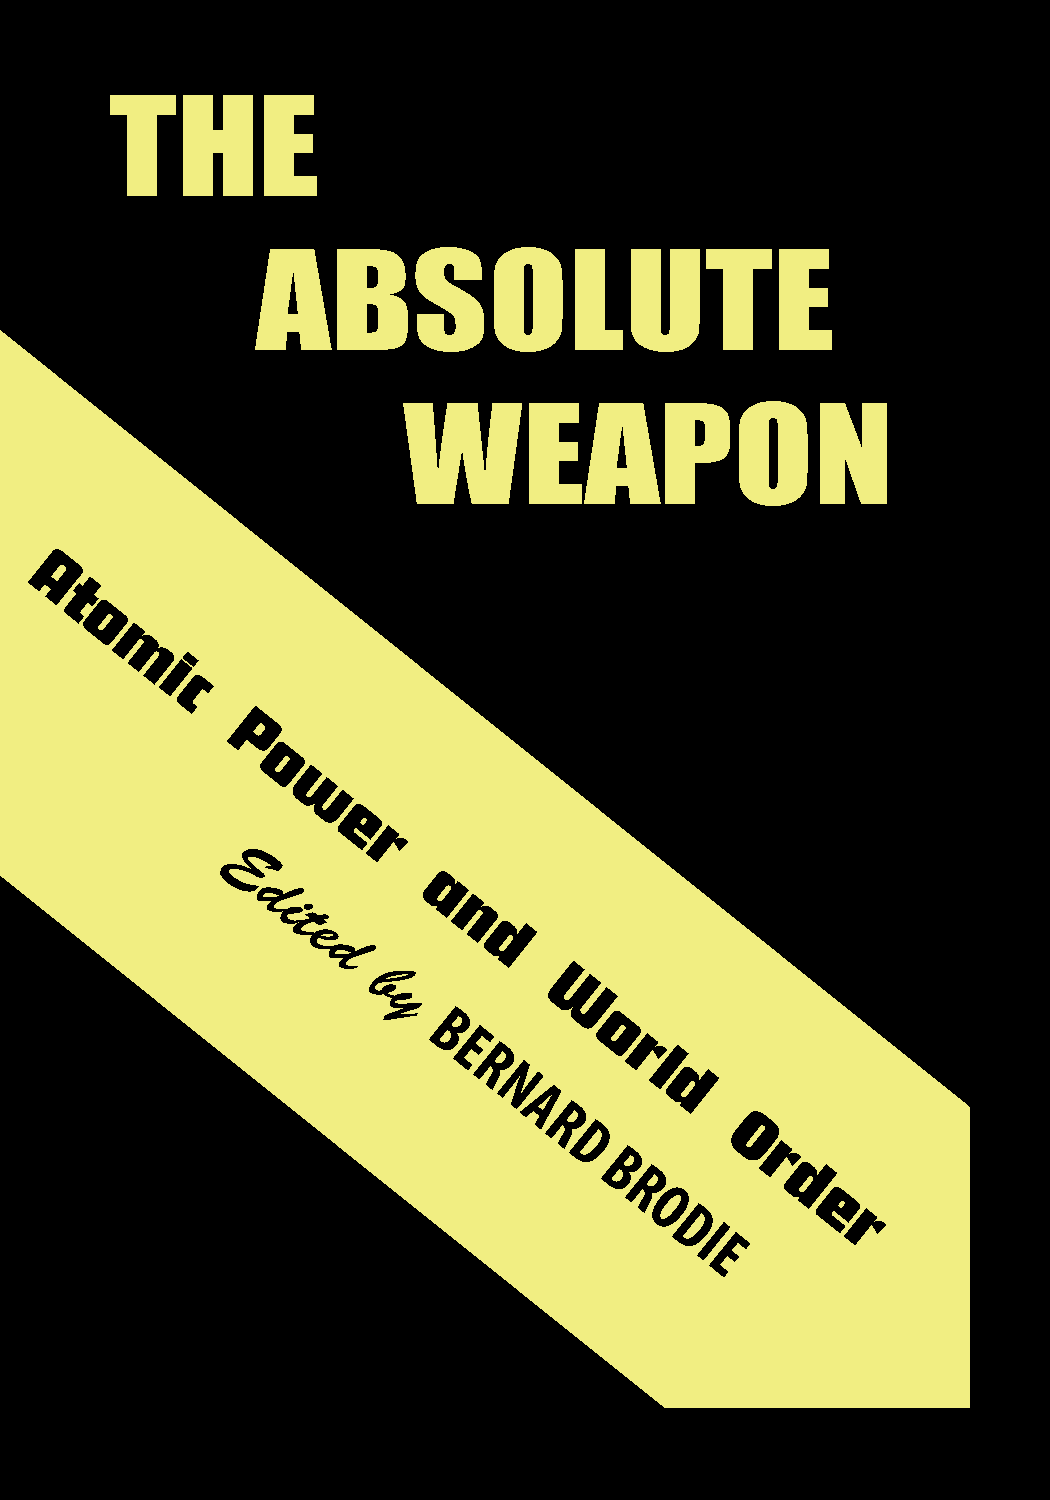
\includepdf[pages={1}, offset = -16.85 0.35]{7x10-cover.pdf}

\thispagestyle{empty}	%This gets rid of the page number on empty page after cover

\frontmatter

\booktitle{The Absolute Weapon}

\subtitle{\Huge{\textit{Atomic Power and World Order}}}

\AuAff{\LARGE{by FREDERICK S. DUNN}\\
\LARGE{\textsc{BERNARD BRODIE $\cdot$ ARNOLD WOLFERS}}\\
\LARGE{\textsc{PERCY E. CORBETT $\cdot$ WILLIAM T. R. FOX}}}

\AuAff{}
\AuAff{\LARGE{Edited by Bernard Brodie}}

%\AuAff{Bernard Brodie, editor\\
%\LARGE{Yale Institute of International Studies}\\
%\LARGE{Frederick S. Dunn, Director}}

\placedate{Yale Institute of International Studies\\
New Haven, Connecticut\\
February 15, 1946}

%% Print Half Title and Title Page:
\halftitlepage
\titlepage

%%%%%%%%%%%%%%%%%%%%%%%%%%%%%%%%%%%%%%%%%%%%%%%%%%%%%%%%%%%%%%%%
%% Copyright Page

%\begin{copyrightpage}{<provide-copyright-year>}
%Title, etc
%\end{copyrightpage}


\tableofcontents



\begin{contributors}

\name{Bernard Brodie,} Yale Institute of International Studies

\name{Arnold Wolfers,} Yale Institute of International Studies

\name{Percy E. Corbett,} Yale Institute of International Studies

\name{William T. R. Fox,} Yale Institute of International Studies

\vspace{20pt}

Introduction by,

\name{Frederick S. Dunn,} Yale Institute of International Studies, Director

\end{contributors}



%%%%%%%%%%%%%%%%%%%%%%%%%%%%%%%%%%%%%%%%%%%%%%%%%%%%%%%%%%%%%%%%
% Optional Acknowledgments:

\acknowledgments
Typeset in \LaTeX~by A. S. Sadek, September 2022.



\begin{introduction}
\addtocontents{toc}{\textit{Frederick S. Dunn}\par}{~}

\vspace{-25pt}

{\huge \textbf{The Common Problem}}

\vspace{40pt}

\noindent{\normalsize \textbf{Frederick S. Dunn}}\\

\vspace{-17pt}
\begin{quote}[poetry]
\raggedleft
``The common problem - yours, mine, everyone's -

Is not to fancy what were fair in life

Provided it could be; but, finding first

What may be, then find how to make it fair

Up to our means - a very different thing!"
\source{\small \textbf{Robert Browning, \textit{Bishop Blougram's Apology}}}
\end{quote}

\vspace{10pt}

Whatever else the successful explosion of the first atomic bomb at Alamagordo signified, it was a victory of the most startling and conclusive sort for scientific research. By a huge effort of combined action, the physical scientists and engineers had succeeded in compressing into a mere sliver of time perhaps several decades of work in applying the energy of the atom to military purposes.

But having achieved this miracle, the scientists themselves were not at all sure that mankind was the gainer by their desperate labors. At least some of them had ardently hoped that their research would prove nothing more than the impossibility of reaching the goal. On the surface of things, the capacity of atomic energy for mass destruction far exceeded any immediately realizable value in enhancing human comfort and welfare. Moreover, like all physical forces, it was morally indifferent and could just as easily serve evil purposes as good. Unless some means could be found for separating out and controlling its powers of annihilation, the scientists' most striking victory of all time threatened on balance to become the heaviest blow ever struck against humanity.

About one thing the physical scientists had no doubt whatever, and that was the surpassing urgency of the problem. They went to extraordinary lengths to stir up the public to a realization of the magnitude of the danger confronting the world. They resorted to extramundane terms to make the non-scientist see that the new physical force was really something different, that it was even a different kind of difference. If they showed perhaps too great a tendency to expect mechanical answers to the problem of how to control this new and terrifying force, that was understandable since they were accustomed to that kind of answer in their own field. But in their efforts to drive home the urgency of the problem, they were serving a high and important purpose.

The more perceptive members of the military profession were equally disturbed, although for slightly different reasons. Whatever value for peacetime uses atomic energy might have, it had been developed as a weapon of war, and its first shattering effects had been felt in that sphere. What bothered the generals and admirals most was the startling efficiency of this new weapon. It was so far ahead of the other weapons in destructive power as to threaten to reduce even the giants of yesterday to dwarf size. In fact to speak of it as just another weapon was highly misleading. It was a revolutionary development which altered the basic character of war itself.

In the pre-atomic days of the 1940's things been bad enough, but one did not have to contemplate very seriously the probable annihilation of both victor and vanquished. Now, even the strongest states were faced with the prospect that they might no longer be able, by their own strength, to save their cities from destruction. Not only might their regular rivals on the same level be equipped with powers of attack hundreds of times greater than before, but possibly some of the nations' lower down in the power scale might get hold of atomic weapons and alter the whole relationship of great and small states. It was becoming very hard to see how a tolerable war could be fought any more.

Unless atomic warfare could be limited, no single state, no matter how strong its military forces might be, could be at all certain to avoid being mortally wounded in a future war. There was not and very likely would not be a sure defense against atomic attack, or any reliable way of keeping bombs away from a nation's territory. A great power might, it is true, by building up to the limit of its strength, have a good chance of winning a war in the end, but what good was that if in the meantime the urban population of the nation had been wiped out? Even military men were beginning to think that perhaps it would be a good idea to look very carefully into the possibilities of restricting atomic warfare by international action.

In any case it was not the task of either the physical scientist or the military strategist to find means of subjecting the new force to effective control. That was clearly a political problem, to be undertaken by the experts in political relationships.

After a few early flights of fancy, most of the political analysts lapsed into a discreet silence on the subject. It was quickly apparent that they had been handed one of the toughest problems which the members of their guild had ever had to face. The profound significance of atomic energy as a physical force called for political thinking on a commensurate scale. Initial probings with the ordinary tools of political analysis brought disappointingly small results. Each sortie into some promising opening either ended up against a solid wall or led into another tangle of seemingly insoluble problems. No clue could be found to a simple formula which would offer repose to men's minds while opening up new vistas of unruffled prosperity. In fact there was reason to believe that nothing of the sort ever would be found and that the job was one of arduous and patient examination of a whole mosaic of related problems extending indefinitely into the future.

One was met right at the beginning with two dilemmas of really imposing dimensions. The first of these arises out of the nature of the procedures available for the common regulation of the actions of free nations. On the one hand, any scheme for international control of atomic warfare must be put into effect by \emph{voluntary} agreement. There is no supreme power to impose it from above. On the other hand, it seemed extremely improbable that states possessing bombs or the capacity to make them would voluntarily restrict their power to carry on atomic warfare merely on the promises of other states to do likewise. Because of the nature of the bomb, any state which broke its word and surreptitiously manufactured atomic weapons could put itself in a position to exert its will over all those who kept their pledge. The more states observed the agreement, the greater the reward to the transgressor.

The second dilemma arises out of the time element in the carrying on of atomic warfare. On the one hand, since no state by its own strength can be sure of staving off a bomb attack, there is a growing conviction that effective control of atomic warfare must come through international action. On the other hand, the speed of attack by bombs can be so great that there would not appear at first sight to be sufficient time for any mechanism of international collective action to operate successfully. Before the air age, one could have counted on a fairly long period of grace between the time when all aggressor's intentions became evident and the time when he could attack in full force. The development of air bombardment shortened this period considerably, and the coming of atomic warfare promises to reduce it almost to zero. If a nation suddenly threatened by atomic bomb attack has to wait while an international agency arrives at a decision as to what counter measures should be taken, the chances of saving its cities would seem to be very small indeed.

Both of these dilemmas are directly concerned with the procedures whereby nations arrive at means of regulating their actions with respect to each other. Both of them receive attention in the chapters that follow. At the present time it is only necessary to make some very general observations about the treaty mechanism and the kinds of strains it might be expected to bear when put to the task of controlling atomic warfare.

Current popular beliefs regarding the efficacy of treaties are prone to be both too optimistic and too pessimistic as to what can be accomplished by them. On the one hand, there is a tendency to believe that practically any international problem can be solved if only the nations concerned can be cajoled into signing a treaty. On the other hand, the spectacular failures of some treaties in the past have led to the widespread conviction that governments in general are very casual about their international obligations and will disregard them whenever they are inconvenient. It is not unusual to find both of these views being held by the same person.

Neither of them finds much support in practice. Those who believe that a treaty is the answer to everything overlook the dreary wasteland of ineffective agreements that have been drafted in disregard of the limits to the loads which the treaty mechanism can bear. Those who make light of treaty commitments in general seem to ignore the fact that the vast majority of such engagements are continuously, honestly, and regularly observed even under adverse conditions and at considerable inconvenience to the parties.

Another common belief is that treaties contain or can be made to contain, single, definite answers to all questions of concrete application, and that strains on treaty observance are merely questions of moral behavior. Treaty failures, in other words, are regarded as lapses in virtue, and it is assumed that the way to avoid them is to strengthen the moral fiber of nations.

It would be foolish to deny that over the years there have been plenty of cases of deliberate bad faith in the non-execution of treaties. The writers on international law have been sighing about it for centuries. Yet it is not helpful just to charge off to the fickleness of sovereigns the many treaty failures that have occurred, and stop there. Most of the time there are quite understandable reasons why treaties fail to work out as expected, and in numerous cases it would be difficult if not impossible to place moral responsibility for such failure.

A good many notorious cases of treaty violation have been concerned with treaties of peace imposed on vanquished nations after a war. Where such treaties place onerous conditions on the losers, as they almost always do, it can be safely predicted that they will be faithfully carried out only so long as the victors have both the power and the inclination to enforce them. Where these grow weak and observance slackens off, the erstwhile victors will certainly cry, ``bad faith" but the other side will see only a just recovery of their former position.

Treaties of alliance have had a decidedly spotty record. Since the possible effect of an alliance is to draw a third party into a war which is not of his doing, the strain on the treaty is very great unless \emph{both} allies feel at the time that they are equally threatened. It seems too much to expect that a nation which has no interest in the outcome of a war will risk its very life merely to fulfill a promise contained in a treaty of alliance. It may well do so if the risk of losing is not very great, but one should not expect this if the odds are clearly against victory.

Where conditions have changed radically and unexpectedly since a treaty was signed, a nation which suffers real injury by such change will on occasion refuse to be bound by its promises. While it is true that under international law the injured state is not justified in doing so without the acquiescence of the other side, nevertheless the absence of any disinterested method of enforcing treaty changes to accord filth changes in surrounding circumstances can cause great hardship and will sometimes induce the injured party to take things into its own hands. In these cases it usually happens that the nation opposing any change will raise aloft the banner of \emph{pacta sunt servanda} as the basic norm of all international relations, yet to the other side it will seem that insistence upon the letter of the treaty is merely black reaction dressed up in the white garments of morality.

Efforts to limit armaments by treaty have certainly not enjoyed a brilliant success. On the other hand, it cannot be said that they have uniformly failed. The more recent criticism leveled against the Washington Treaty for the Limitation of Naval Armament of 1922 was not that it was ineffective but that it was so largely observed. One lesson seems clear and that is that not much can be expected from attempts at limitation of armament which are not closely tied in with the international political pattern of the times or which go counter to the basic policies of any of the top-level powers. It is not so much the ingenuity displayed in working out the details of a disarmament scheme that matters as the way in which it accords with the prevailing balance in the relationships of the powers.

There are many reasons for treaty failure not directly connected with the subject of the treaty itself. Most of these arise out of difficulties of language and uncertainties of intention. Treaties deal with future contingent events. No matter how carefully they are drafted, there are always unforeseen situations arising in which the meaning of the treaty is in doubt. The surrounding circumstances are constantly changing, and every new appearance of an old situation has its degree of novelty. The language by which treaties are drafted is the language of common use, made up of words often heavily laden with ambiguity and possessing extensive twilight zones of murky meaning. The drafters of treaties spend long and dreary days and nights trying to forecast all possible contingencies, yet the ink is scarcely dry on the signatures when new and troublesome situations begin to appear. Each novel case raises a conflict over classification. Statesman White is quite certain that it goes into this verbal category while Statesman Black just as firmly insists that it goes into that one. The fact that each one's interpretation happens to accord with the interests of his own country does not remove the fact that both honestly believe they are right. So far as the dictionaries show, they are.

This fact is familiar enough in the performance of compacts between individuals, but usually there are ample procedures for arriving at a settlement of disputes in accordance with the commonly accepted values of the community. In the international society the procedures are rudimentary and normally cannot be invoked unless both parties, including the one which would gain more by having no decision, consent to the process. Furthermore, the body of universally accepted notions as to what justice requires in the performance of treaties is painfully small.

When one thinks of all the reasons why treaties may fail to fulfill their intended purposes, one may well wonder why nations continue to enter into them. It is said that the first known treaty was made about 3000 B.C. between the kings of Umma and Lagash in settlement of a boundary dispute. No one knows how many treaties have been entered into in the intervening 5000 years but it is undoubtedly a colossal figure. While the total has been liberally sprinkled with instances of bad faith and broken engagements, it is still true that the great majority have been carried out by the parties in good order and have served their respective purposes reasonably well.

Clearly there is nothing in this long experience which compels the conclusion that the treaty process is incapable of bearing the load which would be put upon it by an attempt to control atomic warfare by international action. Treaties are tools which will perform well under certain conditions and badly under others. If a favorable set of conditions can be coaxed into existence, there is no reason to despair of finding a treaty structure that will withstand the strains which are likely to occur.

It is true, nevertheless, that a limitation agreement would fall into the class of treaties which are subjected to the greatest strains, and which not infrequently give way under them. For one thing, the subject matter deals directly with the security of the state, and on such questions every state will, if it can, hold on to the final decision itself. That does not, of course, rule out the possibility of common action, since states are quite capable of appreciating the advantages of such action, but it does put an outside limit on the distance to which a state will go in achieving it.

The greatest strain, of course, would come from the nature of the bomb itself, and the enormous advantage that would be gained by surreptitious violation. So great would be the temptation to evade the treaty that governments would be extremely reluctant to put much faith in it if it rested on nothing more than the reciprocal promises of other states. Before divesting themselves of such a great source of power, they would certainly require assurances that they would be safeguarded against attack by a state that had secretly violated its promises, This is the well-known ``safeguards" problem and it is probably the most difficult one which the atomic energy commission will have to face.

It is in fact a very old problem. The Greeks knew about it, and their system of hostages was in effect a means of assuring fulfillment of treaty terms beyond the mere promise of the signatories.\footnote{This custom continued down to fairly recent times, the last well-known case being that of the Treaty of Aix-la-Chapelle, October 18, 1748, which provided that two English lords were to be handed over to France until the restoration of Cape Breton Island and the English conquests in the East and West Indies. See Coleman Phillipson, \textit{Termination of War and Treaties of Peace}, London, 1916, p. 208.} A safeguard of almost equal antiquity was the oath. This was particularly prevalent in the Middle Ages when religious faith was strong and the spiritual supremacy of the Pope over all sovereigns was universally admitted. The conclusion of treaties was marked by religious ceremonies and the trucing of the oath, the potential violator being threatened with major excommunication. There is no doubt about the fact that this added considerable strength to the sense of obligation of the signatories. But eventually this safeguard lost its power, due partly to a diminution of faith, partly to the changed position of the state in reference to the Church, but perhaps chiefly to the fact that it was not really reliable since the person under oath might possibly be absolved from it.\footnote{See P. C. Borda, \textit{De l'Inex\'ecution des Trait\'es}, Paris, 1922, pp. 37-38.} Nevertheless, the custom has continued down to the present day of using terms of religious significance to give as much weight as possible to treaty obligations, for example, ``the sanctity of treaties", ``solemn covenants solemnly arrived at", ``sacred obligations", etc.

Other forms of safeguards used today are the occupation of territory, as in the case of the Rhineland after the First World War, the guarantee by third powers of the fulfillment of a treaty, and the pledging of certain sources of revenue for the execution of a treaty, as Venezuela did to the European powers in 1902. An interesting form of indirect safeguard is the general exchange of military and naval attaches as a method of removing fears of unfriendly war preparations in derogation of treaties of friendship.

The only one of the familiar safeguards which seems to offer any promise in the international control of atomic energy is that of inspection. If it were possible to back up a limitation agreement with a system of disinterested inspection operating on a world-wide basis, the parties to the agreement would have a way of continuously reassuring themselves that no preparations were under way within any state to evade the agreement. But if this were to be the only safeguard, it would have to be practically infallible, in fact as well as in appearance; otherwise the states living up to the treaty would be lulled into a sense of false security and the door opened to easy violation by a potential troublemaker. Furthermore, unless every state confidently believed in the infallibility of the inspection system, individual nations which had grown suspicious might feel impelled to resort to secret production of atomic weapons as a precautionary measure.

This type of safeguard has a precedent in the inspection system developed in connection with the international control of narcotics.\footnote{This is discussed later in Chapter V, pp. \pageref{V-narco1}-\pageref{V-narco2}.} While this scheme resulted in bringing to light a number of violations, it was by no means infallible, and was scarcely effective at all against violations condoned by national authorities.

Some scientists impressed by the great technical difficulties in the way of a really effective inspection system have taken a very gloomy view of the possibilities of such a safeguard. Others who are more impressed by the problems of concealing the large-scale operations involved in the production of atomic weapons are far less pessimistic. The information so far made available is not sufficient to enable the layman to reach a satisfactory conclusion on the question. Nevertheless one thing seems clear: no one has any doubt but that each state has the power to make certain of what is going on within its own borders in the production and use of fissionable materials. If that is true for every state, then it necessarily follows that global control is not impossible from a technical standpoint, since means could be found for making use of the various national systems as the basis for international control. But this is a political rather than a scientific problem. The members of the atomic energy commission may well find it worth their while to explore it thoroughly.

What all this comes down to is the following: There is no reason to believe that the treaty mechanism is inherently incapable of bearing the load which would be associated with the international control of atomic weapons. Nevertheless, this load would necessarily be very great indeed, and there is no likelihood that nations would willingly narrow their freedom of action in relation to atomic energy merely on the naked promise of other states to do likewise. The potential advantages to be gained by a successful evasion of such a treaty are apparently so stupendous that very powerful safeguards would have to be provided against possible violations. None of the ordinary types of safeguards seem strong enough to provide this assurance.

One possible way of meeting this problem would be to eliminate all existing atomic weapons, destroy all means of production and prohibit all future steps toward production. This idea has wide public support and is in fact set forth in the Truman-Attlee-King declaration and the Moscow resolution as one of the ultimate aims of the work of the atomic energy commission. But in moving in this direction, one is met by a third dilemma of imposing proportions. On the one hand, having no bombs in existence would seem to remove any opportunity to embark on an adventure in atomic warfare. On the other hand, if no bombs are in existence, then any state which successfully evades the agreement and produces bombs would have a complete monopoly of them. Under such conditions the opportunities for world dominance would be breath-taking. Hence we come to the paradox that the further we go by international agreement in the direction of eliminating bombs and installations, the stronger becomes the temptation to evade the agreement. The feeling of security which one imagines would come from a bombless world would seem to be a fleeting one.

This suggests that the basic problem is somewhat different from that of just getting rid of bombs. It is rather a question of how to reduce to the lowest possible minimum the potential advantages to be gained by a successful evasion of a limitation agreement. If the threat to security comes from the prize that is available to a violator of a treaty, then the sensible thing to do would be to take away the value of the prize. Obviously this would not be an easy thing to do, but one has at hand a new and powerful aid for accomplishing it and that is atomic energy itself.

It happens that the atomic bomb is one of the most persuasive deterrents to adventures in atomic warfare that could be devised. It is peculiarly well adapted to the technique of retaliation. One must assume that, so long as bombs exist at all, the states possessing them will hold themselves in readiness at all times for instant retaliation on the fullest possible scale in the event of an atomic attack. The result would be that any potential violator of a limitation agreement would have the terrifying contemplation that not only would he lose his cities immediately on starting an attack, but that his transportation and communication systems would doubtless be gone and his industrial capacity for producing the materials of war would be ruined. If in spite of all this he still succeeded in winning the war, he would find that he had conquered nothing but a blackened ruin. The prize for his violation of his agreement would be ashes!

Hence there does seem to be available a safeguard strong enough to act as a real deterrent against possible evasion of a limitation agreement. But it is powerful medicine and should not be the sole means of assuring the observance of the treaty. Some kind of inspection system would still be extremely helpful. And the first line of defense would always have to be the constant exercise of farsighted, conciliatory diplomacy in order to avoid the building up of tensions that might tempt nations to seek a solution through the use of force. Thus we come to the final paradox that while the best way to avoid atomic warfare is to get rid of war itself, the strongest present ally in the effort to get rid of war is the capacity to resort to atomic warfare at a moment's notice.

\noindent\hfil\rule{0.4\textwidth}{.4pt}\hfil

\vspace{4pt}

The development of the atomic bomb has wrought profound changes in three major fields: (1) in the military affairs of nations, (2) in their political relationships, and (3) in the organized international machinery for peace and security. Each one of these is dealt with in the following text and there is a final chapter on the problem of international control of atomic weapons. There are still large gaps in the information that is essential to arriving at satisfactory answers to specific questions. The authors of the following text are acutely aware of these gaps and are anxious not to claim anything more for their contributions than that they are preliminary essays in an exceedingly difficult and complex subject. But it is time for responsible scholars to speak out to the best of their ability and not wait until all the evidence is in on every question. Only through the hard work of many minds is it likely that the means shall be found to remove the threat of disaster now facing us, a threat the like of which has never been seen before in the history of this planet.

\end{introduction}


\mainmatter

\phantomsection
\addcontentsline{toc}{part}{\fontfamily{cmr}\selectfont \textsc{Part I - The Weapon}}
\part{The Weapon}


\chapter[War in the Atomic Age]{War in the Atomic Age}

\maketitle

\vspace{-2pt}

\noindent{\normalsize \textbf{Bernard Brodie}}

\vspace{39pt}

Most of those who have held the public ear on the subject of the bomb have been content to assume that war and obliteration are now completely synonymous, and that modern man must therefore be either obsolete or fully ripe for the millennium. No doubt the state of obliteration - if that should indeed be the future fate of nations which cannot resolve their disputes - provides little scope for analysis. A few degrees difference in nearness to totality is of relatively small account. But in view of man's historically tested resistance to drastic changes in behavior, especially in a benign direction, one may be pardoned for wishing to examine the various possibilities inherent in the situation before taking any one of them for granted.

It is already known to us all that a war with atomic bombs would be immeasurably more destructive and horrible than any the world has yet known. That fact is indeed portentous, and to many it is overwhelming. But as a datum for the formulation of policy it is in itself of strictly limited utility. It underlines the urgency of our reaching correct decisions, but it does not help us to discover which decisions are in fact correct.

Men have in fact been converted to religion at the point of the sword, but the process generally required actual use of the sword against recalcitrant individuals. The atomic bomb does not lend itself to that kind of discriminate use. The wholesale conversion of mankind away from those parochial attitudes bound up in nationalism is a consummation devoutly to be wished and, where possible, to be actively promoted. But the mere existence of the bomb does not promise to accomplish it at an early enough time to be of any use. The careful handling required to assure long and fruitful life to the Age of Atomic Energy will in the first instance be a function of distinct national governments, not all of which, incidentally, reflect in their behavior the will of the popular majority.

Governments are of course ruled by considerations not wholly different from those which affect even enlightened individuals. That the atomic bomb is a weapon of incalculable horror will no doubt impress most of them deeply. But they have never yet responded to the horrific implications of war in a uniform way. Even those governments which feel impelled to the most drastic self-denying proposals will have to grapple not merely with the suspicions of other governments but with the indisputable fact that great nations have very recently been ruled by men who were supremely indifferent to horror, especially horror inflicted by them on people other than their own.

Statesmen have hitherto felt themselves obliged to base their policies on the assumption that the situation might again arise where to one or more great powers war looked less dangerous or less undesirable than the prevailing conditions of peace. They will want to know how the atomic bomb affects that assumption. They must realize at the outset that a weapon so terrible cannot but influence the degree of probability of war for any given period in the future. But the degree of that influence or the direction in which it operates is by no means obvious. It has, for example, been stated over and over again that the atomic bomb is \emph{par excellence} the weapon of aggression, that it weights the scales overwhelmingly in favor of surprise attack. That if true would indicate that world peace is even more precarious than it was before, despite the greater horrors of war. But is it inevitably true? If not, then the effort to make the reverse true would deserve a high priority among the measures to be pursued.

Thus, a series of questions present themselves. Is war more or less likely in a world which contains atomic bombs? If the latter, is it \emph{sufficiently} unlikely - sufficiently, that is, to give society the opportunity it desperately needs to adjust its politics to its physics? What are the procedures for effecting that adjustment within the limits of our opportunities? And how can we enlarge our opportunities? Can we transpose what appears to be an immediate crisis into a long-term problem, which presumably would permit the application of more varied and better-considered correctives than the pitifully few and inadequate measures which seem available at the moment?

It is precisely in order to answer such questions that we turn our attention to the effect of the bomb on the character of war. We know in advance that war, if it occurs, will be very different from what it was in the past, but what we want to know is: how different, and in what ways? A study of those questions should help us to discover the conditions which will govern the pursuit of world security in the future and the feasibility of proposed measures for furthering that pursuit. At any rate, we know that it is not the mere existence of the weapon but rather its effects on the traditional pattern of war which will govern the adjustments which states will make in their relations with each other.

\noindent\hfil\rule{0.4\textwidth}{.4pt}\hfil

\vspace{4pt}

The Truman-Attlee-King statement of November 15, 1945 epitomized in its first paragraph a few specific conclusions concerning the bomb which have evolved as of that date: ``We recognize that the application of recent scientific discoveries to the methods and practice of war has placed at the disposal of mankind means of military destruction hitherto unknown, against which there can be no adequate military defense, and in the employment of which no single nation can in fact have a monopoly.''

This observation, it would seem, is one upon which all reasonable people would now be agreed. But it should be noted that of the three propositions presented in it the first is either a gross understatement or meaningless, the second has in fact been challenged by persons in high military authority, and the third, while generally admitted to be true, has nevertheless been the subject of violently clashing interpretations. In any case, the statement does not furnish a sufficient array of postulates for the kind of analysis we wish to pursue.

It is therefore necessary to start out afresh and examine the various features of the bomb, its production, and its use which are of military importance. Presented below are a number of conclusions concerning the character of the bomb which seem to this writer to be inescapable. Some of the eight points listed already enjoy fairly universal acceptance; most do not. After offering with each one an explanation of why he believes it to be true, the writer will attempt to deduce from these several conclusions or postulates the effect of the bomb on the character of war.

\begin{enumerate}[I.]

\item \textbf{The power of the present bomb is such that any city in the world can be effectively destroyed by one to ten bombs.}

\end{enumerate}

While this proposition is not likely to evoke much dissent, its immediate implications have been resisted or ignored by important public officials. These implications are two-fold. First, it is now physically possible for air forces no greater than those existing in the recent war to wipe out all the cities of a great nation in a single day - and it will be shown subsequently that what is physically possible must be regarded as tactically feasible. Secondly, with our present industrial organization the elimination of our cities would mean the elimination for military purposes of practically the whole of our industrial structure. But before testing these extraordinary implications, let us examine and verify the original proposition.

The bomb dropped on Hiroshima completely pulverized an area of which the radius from the point of detonation was about one and one-quarter miles. However, everything within a radius of two miles was blasted with some burning and between two and three miles the buildings were about half destroyed. Thus the area of total destruction covered about four square miles, and the area of destruction and substantial damage extended over some twenty-seven square miles. The bomb dropped on Nagasaki, while causing less damage than the Hiroshima bomb because of the physical characteristics of the city, was nevertheless considerably more powerful. We have it on Dr. J. Robert Oppenheimer's authority that the Nagasaki bomb ``would have taken out ten square miles, or a bit more, if there had been ten square miles to take out.''\footnote{``Atomic Weapons and the Crisis in Science'', \textit{Saturday Review of Literature}, November 24, 1945, p. 10.} From the context in which that statement appears it is apparent that Dr. Oppenheimer is speaking of an area of total destruction.

The city of New York is listed in the \emph{World Almanac} as having an area of 365 square miles. But it obviously would not require the pulverization of every block of it to make the whole area one of complete chaos and horror. Ten well-placed bombs of the Nagasaki type would eliminate that city as a contributor to the national economy, whether for peace or war, and convert it instead into a catastrophe area in dire need of relief from outside. If the figure of ten bombs be challenged, it need only be said that it would make very little difference militarily if twice that number of bombs were required. Similarly, it would be a matter of relative indifference if the power of the bomb were so increased as to require only five to do the job. Increase of power in the individual bomb is of especially little moment to cities of small or medium size, which would be wiped out by one bomb each whether that bomb were of the Nagasaki type or of fifty times as much power. No conceivable variation in the power of the atomic bomb could compare in importance with the disparity in power between atomic and previous types of explosives.

The condition at this writing of numerous cities in Europe and Japan sufficiently underlines the fact that it does not require atomic bombs to enable man to destroy great cities. TNT and incendiary bombs when dropped in sufficient quantities are able to do a quite thorough job of it. For that matter, it should be pointed out that a single bomb which contains in itself the concentrated energy of 20,000 tons of TNT is by no means equal in destructive effect to that number of tons of TNT distributed among bombs of one or two tons each. The destructive radius of any one bomb increases only with the cube root of the explosive energy released, and thus the very concentration of power in the atomic bomb detracts from its overall effectiveness. The bomb must be detonated from an altitude of at least 1,000 feet if the full spread of its destructive radius is be to realized, and much of the blast energy is absorbed by the air above the target. But the sum of initial energy is quite enough to afford such losses.

If should be obvious that there is much more than a logistic difference involved between a situation where a single plane sortie can cause the destruction of a city like Hiroshima and one in which at least 500 bomber sorties are required to do the same job. Nevertheless, certain officers of the U.S. Army Air Forces, in an effort to ``deflate'' the atomic bomb, have observed publicly enough to have their comments reported in the press that the destruction wrought at Hiroshima could have been effected by two days of routine bombing with ordinary bombs. Undoubtedly so, but the 500 or more bombers needed to do the job under those circumstances would if they were loaded with atomic bombs be physically capable of destroying 500 or more Hiroshimas in the same interval of time. That observation discounts certain tactical considerations. These will be taken up in due course, but for the moment it is sufficient to point out that circumstances do arise in war when it is the physical carrying capacity of the bombing vehicles rather than tactical considerations which will determine the amount of damage done.

\begin{enumerate}[resume*]

\item \textbf{No adequate defense against the bomb exists, and the possibilities of its existence in the future are exceedingly remote.}

\end{enumerate}

This proposition requires little supporting argument in so far as it is a statement of existing fact. But that part of it which involves a prediction for the future conflicts with the views of most of the high-ranking military officers who have ventured opinions on the implications of the atomic bomb. No layman can with equanimity differ from the military in their own field, and the present writer has never entertained the once-fashionable view that the military do not know their own business. But, apart from the question of objectivity concerning professional interests - in which respect the record of the military profession is neither worse nor better than that of other professions - the fact is that the military experts have based their arguments mainly on presumptions gleaned from a field in which they are generally not expert, namely, military \emph{history}. History is at best an imperfect guide to the future, but when imperfectly understood and interpreted it is a menace to sound judgment.

The defense against hostile missiles in all forms of warfare, whether on land, sea, or in the air, has thus far depended basically on a combination of, first, measures to reduce the number of missiles thrown or to interfere with their aim (i.e., defense by offensive measures) and, secondly, ability to absorb those which strike. To take an obvious example, the large warship contains in itself and in its escorting air or surface craft a volume of fire power which usually reduces and may even eliminate the blows of the adversary. Unlike most targets ashore, it also enjoys a mobility which enables it to maneuver evasively under attack (which will be of no value under atomic bombs). But unless the enemy is grotesquely inferior in strength, the ship's ability to survive must ultimately depend upon its compartmentation and armor, that is, on its ability to absorb punishment.

The same is true of a large city. London was defended against the German V-1 or ``buzz-bomb'' first by concerted bombing attacks upon the German experimental stations, industrial plants, and launching sites, all of which delayed the V-1 attack and undoubtedly greatly reduced the number of missiles ultimately launched. Those which were nevertheless launched were met by a combination of fighter planes, antiaircraft guns, and barrage balloons. Towards the end of the eighty-day period which covered the main brunt of the attack, some 75 per cent of the bombs launched were being brought down, and, since many of the remainder were inaccurate in their flight, only 9 per cent were reaching London.\footnote{Duncan Sandys, \textit{Report on the Flying Bomb}, pamphlet issued by the British Information Services, September, 1944, p. 9.} These London was able to ``absorb''; that is, there were casualties and damage but no serious impairment of the vital services on which depended the city's life and its ability to serve the war effort.

It is precisely this ability to absorb punishment, whether one is speaking of a warship or a city, which seems to vanish in the face of atomic attack. For almost any kind of target selected, the so-called ``static defenses'' are defenses no longer. For the same reason too, mere reduction in the number of missiles which strike home is not sufficient to save the target, though it may have some effect on the enemy's selection of targets. The defense of London against V-1was considered effective, and yet in eighty days some 2,300 of those missiles hit the city. The record bag was that of August 28, 1944, when out of 101 bombs which approached England 97 were shot down and only four reached London. But if those four had been atomic bombs, London survivors would not have considered the record good. Before we can speak of a defense against atomic bombs being effective, \label{I-frustrate} \emph{the frustration of the attack for any given target area must be complete}. Neither military history nor an analysis of present trends in military technology leaves appreciable room for hope that means of completely frustrating attack by aerial missiles will be developed.

In his speech before the Washington Monument on October 5, 1945, Fleet Admiral Chester W. Nimitz correctly cautioned the American people against leaping to the conclusion that the atomic bomb had made armies and navies obsolete. But he could have based his cautionary note on better grounds than he in fact adopted. ``Before risking our future by accepting these ideas at face value,'' he said, ``let us examine the historical truth that, at least up to this time, there has never yet been a weapon against which man has been unable to devise a counter-weapon or a defense.\footnote{For the text of the speech see the \textit{New York Times}, October 6, 1945, p. 6. See also the speech of President Truman before Congress on October 23, 1945, in which he said: ``Every new weapon will eventually bring some counter-defense against it.''}

Apart from the possible irrelevancy for the future of this observation - against which the phrase ``at least up to this time'' provides only formal protection - the fact is that it is not historically accurate. A casual reading of the history of military technology does, to be sure, encourage such a doctrine. The naval shell gun of 1837, for example, was eventually met with iron armor, and the iron armor in turn provoked the development of the ``built-up'' gun with greater penetrating power; the submarine was countered with the hydrophone and supersonic detector and with depth charges of various types; the bombing airplane accounted for the development of the specialized fighter aircraft, the highly perfected antiaircraft gun, and numerous ancillary devices. So it has always been, and the tendency is to argue that so it always will be.

In so far as this doctrine becomes dogma and is applied to the atomic bomb, it becomes the most dangerous kind of illusion. We have already seen that the defense against the V-1 was only \emph{relatively} effective, and something approaching much closer to perfect effectiveness would have been necessary for V-1 missiles carrying atomic bombs. As a matter of fact, the defense against the V-2 rocket were of practically zero effectiveness, and those who know most about it admit that thus far there has been no noteworthy progress against the V-2.\footnote{See Ivan A. Getting, ``Facts About Defense,'' \textit{Nation}, Special Supplement, Dec. 22, 1945, p. 704. Professor Getting played a key part in radar development for antiaircraft work and was especially active in measures taken to defend London against V-1 and V-2.}

These, to be sure, were new weapons. But what is the story of the older weapons? After five centuries of the use of hand arms with fire-propelled missiles, the large numbers of men killed by comparable arms in the recent war indicates that no adequate answer has yet been found for the bullet.\footnote{The new glass-fiber body armor, ``Doron'', will no doubt prove useful but is not expected to be of more than marginal effectiveness.} Ordinary TNT, whether in shell, bomb, or torpedo, can be ``countered'' to a degree by the dispersion of targets or by various kinds of armor, but the enormous destruction wrought by this and comparable explosives on land, sea, and in the air in World War II is an eloquent commentary on the limitations of the defenses. The British following the first World War thought they had in their ``Asdic'' and depth charges the complete answer to the U-boat, but an only slightly improved U-boat succeeded in the recent war in sinking over 23 million gross tons of shipping. So the story might go on endlessly. It has simply become customary to consider an ``answer'' satisfactory when it merely diminishes or qualifies the effectiveness of the weapon against which it is devised, and that kind of custom will not do for the atomic bomb.

Despite such statements as that of Canadian General A. G. L. McNaughton that means with which to counter the atomic bomb area already ``clearly in sight'',\footnote{\textit{New York Herald Tribune}, October 6, 1945, p. 7.} it seems pretty well established that there is no \emph{specific} reply to the bomb. The physicists and chemists who produced the atomic bomb are apparently unanimous on this point: that while there was a scientific consensus long before the atomic bomb existed that it could be produced, no comparable opinion is entertained among scientists concerning their chances of devising effective counter-measures. The bomb itself is as free from direct interference of any kind as is the ordinary bomb. When the House Naval Affairs Committee circulated a statement that electronic means were already available for exploding atomic bombs ``far short of their objective without the necessity of locating their position'',\footnote{\textit{New York Times}, October 12, 1945, p. 1.} scientists qualified to speak promptly denied this assertion and it was even disowned by its originators.

Any active defense at all must be along the lines of affecting the carrier, and we have already noted that even when used with the relatively vulnerable airplane or V-1 the atomic bomb poses wholly new problems for the defense. A nation which had developed strong defenses against invading aircraft, which had found reliable means of interfering with radio-controlled rockets, which had developed highly efficient counter-smuggling and counter-sabotage agencies, and which had dispersed through the surrounding countryside substantial portions of the industries and populations normally gathered in urban communities would obviously be better prepared to resist atomic attack than a nation which had either neglected or found itself unable to do these things. But it would have only a relative advantage over the latter; it would still be exposed to fearful destruction.

In any case, technological progress is not likely to be confined to measures of defense. The use of more perfect vehicles and of more destructive bombs in greater quantity might very well offset any gains in defense. And the bomb already has a fearful lead in the race.

Random and romantic reflections on the miracles which science has already wrought are of small assistance in our speculations on future trends. World War II saw the evolution of numerous instruments of war of truly startling ingenuity. But with the qualified exception of the atomic bomb itself (the basic principle of which was discovered prior to but in the same year of the outbreak of war in Europe), all were simply mechanical adaptations of scientific principles which were well known long before the war. It was no doubt a long step from the discovery in 1922 of the phenomenon upon which radar is based to the use of the principle in an antiaircraft projectile fuse, but here too realization that it might be so used considerably antedated the fuse itself.

The advent of a ``means of destruction hitherto unknown'' - to quote the Truman-Attlee-King statement - is certainly not new. The steady improvement of weapons of war is an old story, and the trend in that direction has in recent years been accelerated. But thus far each new implement has, at least initially, been limited enough in the scope of its use or in its strategic consequences to permit some timely measure of adaptation both on the battlefield and in the minds of strategists and statesmen. Even the most ``revolutionary'' developments of the past seem by contrast with the atomic bomb to have been minor steps in a many-sided evolutionary process. This process never permitted any one invention in itself to subvert or even to threaten for long the previously existing equilibrium of military force. Any startling innovation either of offense or defense provoked some kind of answer in good time, but the answer was rarely more than a qualified one and the end result was usually a profound and sometimes a politically significant change in the methods of waging war.\footnote{For a discussion of developing naval technology over the last hundred years and its political significance see Bernard Brodie, \textit{Sea Power in the Machine Age}, Princeton, N.J., 2nd. ed. 1943.}

With the introduction, however, of an explosive agent which is several million times more potent on a pound for pound basis than the most powerful explosives previously known, we have a change of quite another character. The factor of increase of destructive efficiency is so great that there arises at once the strong presumption that the experience of the past concerning eventual adjustment might just as well be thrown out the window. Far from being something which merely ``adds to the complexities of field commanders'', as one American military authority put it, the atomic bomb seems so far to overshadow any military invention of the past as to render comparison ridiculous.

\begin{enumerate}[resume*]

\item \textbf{The atomic bomb not only places an extraordinary military premium upon the development of new types of carriers but also greatly extends the destructive range of existing carriers.}

\end{enumerate}

World War II saw the development and use by the Germans of rockets capable of 220 miles range and carrying approximately one ton each of TNT. Used against London, these rockets completely baffled the defense. But for single-blow weapons which were generally inaccurate at long distances even with radio control, they were extremely expensive. It is doubtful whether the sum of economic damage done by these missiles equalled the expenditure which the Germans put into their development, production, and use. At any rate, the side enjoying command of the air had in the airplane a much more economical and longer-range instrument for inflicting damage on enemy industry than was available in the rocket. The capacity of the rocket-type projectile to strike without warning in all kinds of weather with complete immunity from all known types of defenses guaranteed to it a supplementary though subordinate role to bomber-type aircraft. But its inherent limitations, so long as it carried only chemical explosives, were sufficient to warrant considerable reserve in predictions of its future development.

\label{I-range1}

However, the power of the new bomb completely alters the considerations which previously governed the choice of vehicles and the manner of using them. A rocket far more elaborate and expensive than the V-2 used by the Germans is still an exceptionally cheap means of bombarding a country if it can carry in its nose an atomic bomb. The relative inaccuracy of aim - which continued research will no doubt reduce - is of much diminished consequence when the radius of destruction is measured in miles rather than yards. And even with existing fuels such as were used in the German V-2, it is theoretically feasible to produce rockets capable of several thousands of miles of range, though the problem of \emph{controlling} the flight of rockets over such distances is greater than is generally assumed.

Of more immediate concern than the possibilities of rocket development, however, is the enormous increase in effective bombing range which the atomic bomb gives to \emph{existing types of aircraft}. That it has this effect becomes evident when one examines the various factors which determine under ordinary - that is, non-atomic bomb - conditions whether a bombing campaign is returning military dividends. First, the campaign shows profit only if a large proportion of the planes, roughly 90 per cent or more, are returning from individual strikes.\footnote{The actual figure of loss tolerance depends on a number of variables, including replacement rate of planes and crews, morale factors, the military value of the damage being inflicted on the enemy, and the general strategic position at the moment. The 10 per cent figure used for illustration in the text above was favored by the war correspondents and press analysts during the recent war, but it must not be taken too literally.} Otherwise one's air force may diminish in magnitude more rapidly than the enemy's capacity to fight. Each plane load of fuel must therefore cover a two-way trip, allowing also a fuel reserve for such contingencies as adverse winds and combat action, thereby diminishing range by at least one-half from the theoretical maximum.

But the plane cannot be entirely loaded with fuel. It must also carry besides its crew a heavy load of defensive armor and armament. Above all, it must carry a sufficient load of bombs to make the entire sortie worth while - a sufficient load, that is, to warrant attendant expenditures in fuel, engine maintenance, and crew fatigue. The longer the distance covered, the smaller the bomb load per sortie and the longer the interval between sorties. To load a plane with thirty tons of fuel and only two tons of bombs, as we did in our first B-29 raid on Japan, will not do for a systematic campaign of strategic bombing. One must get closer to the target and thus transfer a greater proportion of the carrying capacity from fuel to bombs.\footnote{It should be noticed that in the example of the B-29 raid of June 15, 1944, cited above, a reduction of only one-fourth in the distance and therefore in the fuel load could make possible (unless the plane was originally overloaded) a tripling or quadrupling of the bomb load. Something on that order was accomplished by our seizure of bases in the Mariannas, some 300 miles closer to the target than the original Chinese bases and of course much easier supplied. The utility of the Mariannas bases was subsequently enhanced by our capture of Iwo Jima and Okinawa, which served as emergency landing fields for returning B-29s and also as bases for escorting fighters and rescue craft. Towards the end of the campaign we were dropping as much as 6,000 tons of bombs in a single raid on Tokyo, thereby assuring ourselves high military dividends per sortie investment.} What we then come out with is an effective bombing range less than one-fourth the straight-line cruising radius of the plane under optimum conditions. In other words a plane capable, without too much stripping of its equipment, of a 6,000-mile non-stop flight would probably have an effective bombing range of substantially less than 1,500 miles.

With atomic bombs, however, the considerations described above which so severely limit bomb range tend to vanish. There is no question of increasing the number of bombs in order to make the sortie profitable. One per plane is quite enough. The gross weight of the atomic bomb is secret, but even if it weighed two to four tons it would still be a light load for a B-29. It would certainly be a sufficient pay load to warrant any conceivable military expenditure on a single sortie. The next step then becomes apparent. Under the callously utilitarian standards of military bookkeeping, a plane and its crew can very well be sacrificed in order to deliver an atomic bomb to an extreme distance. We have, after all, the recent and unforgettable experience of the Japanese \textit{Kamikaze}.\footnote{On several occasions the U.S. Army Air Forces also demonstrated its willingness to sacrifice availability of planes and crews - though not the lives of the latter - in order to carry out specific missions. Thus in the Doolittle raid against Japan of April 1942, in which sixteen Mitchell bombers took off from the carrier \textit{Hornet} it was known beforehand that none of the planes would be recovered even if they succeeded in reaching China (which several failed to do for lack of fuel) and that the members of the crews were exposing themselves to uncommon hazard. And the cost of the entire expedition was accepted mainly for the sake of dropping 16 tons of ordinary bombs! Similarly, several of the Liberators which bombed the Ploesti oil fields in August 1943 had insufficient fuel to return to their bases in North Africa and, as was foreseen, had to land in neutral Turkey where planes and crews were interned.} Thus, the plane can make its entire flight in one direction, and its range would be almost as great with a single atomic bomb as it would be with no bomb load whatever. The non-stop flight during November 1945 of a B-29 from Guam to Washington, D.C., almost 8,200 statute miles, was in this respect more than a stunt. It was a rough indication of the extreme \emph{effective} bombing range with atomic bombs of types of aircraft already in use.\footnote{See \textit{New York Times}, November 21, 1945, p. 1. It should be noticed that the plane had left about 300 gallons, or more than one ton, of gasoline upon landing in Washington. It was of course stripped of all combat equipment (e.g., armor, guns, ammunition, gun-directors, and bomb-sights) in order to allow for a greater gasoline load. Planes bent on a bombing mission would probably have to carry some of this equipment, even if their own survival was not an issue, in order to give greater assurance of their reaching the target.}

Under the conditions just described, any world power is able from bases within its own territories to destroy all the cities of any other world power. It is \emph{not} necessary, despite the assertions to the contrary of various naval and political leaders including President Truman, to seize advanced bases close to enemy territory as a prerequisite to effective use of the bomb.\footnote{See President Truman's speech before Congress on the subject of universal military training, reported in the \textit{New York Times}, October 24, 1945, p. 3.} The lessons of the recent Pacific war in that respect are not merely irrelevant but misleading, and the effort to inflate their significance for the future is only one example of the pre-atomic thinking prevalent today even among people who understand fully the power of the bomb. To recognize that power is one thing; to draw out its full strategic implications is quite another.

The facts just presented do not mean that distance loses all its importance as a barrier to conflict between the major power centers of the world. It would still loom large in any plans to consolidate an atomic bomb attack by rapid invasion and occupation. It would no doubt also influence the success of the bomb attack itself. Rockets are likely to remain of lesser range than aircraft and less accurate near the limits of their range, and the weather hazards which still affect aircraft multiply with distance. Advanced bases will certainly not be valueless. But it is nevertheless a fact that under existing technology the distance separating, for example, the Soviet Union from the United States offers no direct immunity to either with respect to atomic bomb attack, though it does so for all practical purposes with respect to ordinary bombs.\footnote{Colonel Clarence S. Irvine, who commanded the plane which flew non-stop from Guam to Washington, was reported by the press as declaring that one of the objects of the flight was ``to show the vulnerability of our country to enemy air attack from vast distances.'' \textit{New York Times}, November 21, 1945, p. 1.}

\label{I-range2}

\begin{enumerate}[resume*]

\item \textbf{Superiority in air forces, though a more effective safeguard in itself than superiority in naval or land forces, nevertheless fails to guarantee security.}

\end{enumerate}

This proposition is obviously true in the case of very long range rockets, but let us continue to limit our discussion to existing carriers. In his \textit{Third Report to the Secretary of War}, dated November 12, 1945, General H. H. Arnold, commanding the Army Air Forces, made the following statement: ``Meanwhile [i.e., until very long range rockets are developed], the only known effective means of delivering atomic bombs in their present stage of development is the very heavy bomber, and that is certain of success only when the user has air superiority''.\footnote{See printed edition of the \textit{Report}, p. 68. In the sentence following the one quoted, General Arnold adds that this statement is ``perhaps true only temporarily'', but it is apparent from the context that the factor he has in mind which might terminate its ``truthfulness'' is the development of rockets comparable to the V-2 but of much longer range. The present discussion is not concerned with rockets at all.}

This writer feels no inclination to question General Arnold's authority on matters pertaining to air combat tactics. However, it is pertinent to ask just what the phrase ``certain of success'' means in the sentence just quoted, or rather, how much certainty of success is necessary for each individual bomb before. an atomic bomb attack is considered feasible. In this respect one gains some insight into what is in General Arnold's mind from a sentence which occurs somewhat earlier on the same page in the \textit{Report}: ``Further, the great unit cost of the atomic bomb means that as nearly as possible every one must be delivered to its intended target.'' Here is obviously the major premise upon which the conclusion above quoted is based, and one is not disputing General Arnold's judgment in the field of his own specialization by examining a premise which lies wholly outside of it.

When the bombs were dropped on Hiroshima and Nagasaki in August 1945, there were undoubtedly very few such bombs in existence - which would be reason enough for considering each one precious regardless of cost. But their development and production up to that time amounted to some 2 billions of dollars, and that figure would have to be divided by the number made to give the cost of each. If, for example, there were 20 in existence, the unit cost would have to be reckoned at \$100,000,000. That, indeed, is a staggering sum for one missile, being approximately equivalent to the cost of one \emph{Iowa} class battleship. It is quite possible that there were fewer than 20 at that time, and that the unit cost was proportionately higher. For these and other reasons, including the desirability for psychological effect of making certain that the initial demonstration should be a complete success, one can understand why it was then considered necessary, as General Arnold feels it will remain necessary, to ``run a large air operation for the sole purpose of delivering one or two atomic bombs.''\footnote{\emph{Ibid}., p. 68.}

But it is of course clear that as our existing plant is used for the production of more bombs - and it has already been revealed that over three-fourths of the 2 billion dollars went into capital investment for plants and facilities\footnote{According to the figures provided the MacMahon Committee by Major General Leslie R. Groves, the total capital investment spent and committed for plants and facilities as of June 30, 1945 was \$1,595,000,000. Total operating costs up to the time the bombs were dropped in August were \$405,000,000. The larger sum is broken down as follows:

\vspace{10pt}

\begin{tabular}{@{}lr@{}}
\toprule
Manufacturing facilities alone				&	\$1,242,000,000\\
Research								&	\$186,000,000\\
Housing for workers						&	\$162,500,000\\
Workmen's compensation and medical care	&	\$4,500,000\\
\midrule
\textbf{Total}							&	\$1,595,000,000\\
\botrule
\end{tabular}

\vspace{10pt}

One might question the inclusion of the last item as a part of ``capital investment'', but it is in any case an insignificant portion of the whole.} - the unit cost will decline. Professor Oppenheimer has estimated that even with existing techniques and facilities, that is, allowing for no improvements whatever in the production processes, the unit cost of the bomb should easily descend to something in the neighborhood of \$1,000,000.\footnote{\textit{loc. cit.}, p. 10.}

Now a million dollars is a large sum of money for any purpose other than war. Just what it means in war may be gauged by the fact that it amounts to substantially less than the cost of two fully equipped Flying Fortresses (B-17s, not B-29s), a considerable number of which were expended in the recent war without waiting upon situations in which each sortie would be certain of success. The money cost of the war to the United States was sufficient to have paid for 2 or 3 hundred thousand of our million dollar bombs. It is evident, therefore, that in the future it will not be the unit cost of the bomb but the number of bombs actually available which will determine the acceptable wastage in any atomic bomb attack.\footnote{This discussion recalls the often repeated canard that admirals have been cautious of risking battleships in action because of their cost. The 13 old battleships and 2 new ones available to us just after Pearl Harbor reflected no great money value, but they were considered precious because they were scarce and irreplaceable. Later in the war, when new battleships had joined the fleet and when we had eliminated several belonging to the enemy, no battleships were withheld from any naval actions in which they could be of service. Certainly they were not kept out of the dangerous waters off Normandy, Leyte, Luzon, and Okinawa.}

Thus, if Country A should have available 5,000 atomic bombs, and if it should estimate that 500 bombs dropped on the cities of Country B would practically eliminate the industrial plant of the latter nation, it could afford a wastage of bombs of roughly 9 to 1 to accomplish that result. If its estimate should prove correct and if it launched an attack on that basis, an expenditure of only 5 billions of dollars in bombs would give it an advantage so inconceivably overwhelming as to make easy and quick victory absolutely assured - provided it was able somehow to prevent retaliation in kind. The importance of the latter proviso will be elaborated in the whole of the following chapter. Meanwhile it should be noted that the figure of 5,000 bombs cited above is, as will shortly be demonstrated, by no means an impossible or extreme figure for any great power which has been producing atomic bombs over a period of ten or fifteen years.

To approach the same point from another angle, one might take an example from naval warfare. The commander of a battleship will not consider the money cost of his 16-inch shells (perhaps \$3,000 each at the gun's breech) when engaging an enemy battleship, He will not hesitate, at least not for financial reasons, to open fire at extreme range, even if he can count on only one hit in thirty rounds. The only consideration which could give him pause would be the fear of exhausting his armor-piercing ammunition before he has sunk or disabled the enemy ship. The cost of each shell, to be sure, is much smaller than the cost of one atomic bomb, but the amount of damage each hit accomplishes is also smaller - disproportionately smaller by a wide margin.

In calculations of acceptable wastage, the money cost of a weapon is usually far overshadowed by considerations of availability; but in so far as it does enter into those calculations, it must be weighed against the amount of damage done the enemy with each hit. A million dollar bomb which can do a billion dollars worth of damage - and that is a conservative figure - is a very cheap missile indeed. In fact, one of the most frightening things about the bomb is that it makes the destruction of enemy cities an immeasurably cheaper process than it was before, cheaper not alone in terms of missiles but also in terms of the air forces necessary to do the job. Provided the nation using them has enough such bombs available, it can afford a large number of misses for each hit obtained.

To return to General Arnold's observation, we know from the experience of the recent war that very inferior air forces can penetrate to enemy targets if they are willing to make the necessary sacrifices. The Japanese aircraft which raided Pearl Harbor were considerably fewer in number than the American planes available at Pearl Harbor. That, to be sure, was a surprise attack preceding declaration of hostilities, but such possibilities must be taken into account for the future. At any rate, the Japanese air attacks upon our ships off Okinawa occurred more than 3 years after the opening of hostilities, and there the Japanese, who were not superior in numbers on any one day and who did indeed lose over 4,000 planes in 2 months of battle, nevertheless succeeded in sinking or damaging no fewer than 253 American warships. For that matter, the British were effectively raiding targets deep in Germany, and doing so without suffering great casualties, long before they had overtaken the German lead in numbers of aircraft. The war has demonstrated beyond the shadow of a doubt that the sky is much too big to permit one side, however superior, to shut out enemy aircraft completely from the air over its territories.

The concept of ``command of the air'', which has been used altogether too loosely, has never been strictly analogous to that of ``command of the sea''. The latter connotes something approaching absolute exclusion of enemy surface craft from the area in question. The former suggests only that the enemy is suffering losses greater than he can afford, whereas one's own side is not. But the appraisal of tolerable losses is in part subjective, and is also affected by several variables which may have little to do with the number of planes downed. Certainly the most important of those variables is the amount of damage being inflicted on the bombing raids. An air force which can destroy the cities in a given territory has for all practical purposes the fruits of command of the air, regardless of its losses.

Suppose, then, one put to the Army Air Forces the following question: If 3,000 enemy bombers flying simultaneously but individually (i.e., completely scattered)\footnote{The purpose of the scattering would be simply to impose maximum confusion on the superior defenders. Some military airmen have seriously attempted to discount the atomic bomb with the argument that a hit upon a plane carrying one would cause the bomb to explode, blasting every other plane for at least a mile around out of the air. That is not why formation flying is rejected in the example above. Ordinary bombs are highly immune to such mishaps, and from all reports of the nature of the atomic bomb it would seem to be far less likely to undergo explosion as a result even of a direct hit.} invaded our skies with the intention of dividing between them as targets most of the 92 American cities which contain a population of 100,000 or over (embracing together approximately 29 per cent of our total population), if each of those planes carried an atomic bomb, and if we had 9,000 alerted fighters to oppose them, how much guarantee of protection could be accorded those cities? The answer would undoubtedly depend on a number of technical and geographic variables, but under present conditions it seems to this writer all too easy to envisage situations in which few of the cities selected as targets would be spared overwhelming destruction.

That superiority which results in the so-called ``command of the air'' is undoubtedly necessary for successful strategic bombing with ordinary bombs, where the weight of bombs required is so great that the same planes must be used over and over again. In a sense also (though one must register some reservations about the exclusion of other arms) General Arnold is right when he says of atomic bomb attack: ``For the moment, at least, absolute air superiority in being at all times, combined with the best antiaircraft ground devices, is the only form of defense that offers any security whatever, and it must continue to be an essential part of our security program for a long time to come.''\footnote{\textit{Ibid}., p. 68.} But it must be added that the ``only form of defense that offers any security whatever'' falls far short, even without any consideration of rockets, of offering the already qualified kind of security it formerly offered.

\begin{enumerate}[resume*]

\item \textbf{Superiority in numbers of bombs is not in itself a guarantee of strategic superiority in atomic bomb warfare.}

\end{enumerate}

\label{I-SuperiorNos1}

Under the technical conditions apparently prevailing today, and presumably likely to continue for some time to come, the primary targets for the atomic bomb will be cities. One does not shoot rabbits with elephant guns, especially if there are elephants available. The critical mass conditions to which the bomb is inherently subject place the minimum of destructive energy of the individual unit at far too high a level to warrant its use against any target where enemy strength is not already densely concentrated. Indeed, there is little inducement to the attacker to seek any other kind of target. If one side can eliminate the cities of the other, it enjoys an advantage which is practically tantamount to final victory, provided always its own cities are not similarly eliminated.

The fact that the bomb is inevitably a weapon of indiscriminate destruction will carry no weight in any war in which it is used. Even in World War II, in which the bombs used could to a large extent isolate industrial targets from residential districts within an urban area, the distinctions imposed by international law between ``military'' and ``non-military'' targets disintegrated entirely.\footnote{This was due in part to deliberate intention, legally permitted on the Allied side under the principle of retaliation, and in part to a desire of the respective belligerents to maximize the effectiveness of the air forces available to them. ``Precision bombing'' was always a misnomer, though some selectivity of targets was possible in good weather. However, such weather occurred in Europe considerably less than half the time, and if the strategic air forces were not to be entirely grounded during the remaining time they were obliged to resort to ``area bombing''. Radar, when used, was far from being a substitute for the human eye.}

How large a city has to be to provide a suitable target for the atomic bomb will depend on a number of variables - the ratio of the number of bombs available to the number of cities which might be hit, the wastage of bombs in respect to each target, the number of bombs which the larger cities can absorb before ceasing to be profitable targets, and, of course, the precise characteristics and relative accessibility of the individual city. Most important of all is the place of the particular city in the nation's economy. We can see at once that it does not require the obliteration of all its towns to make a nation wholly incapable of defending itself in the traditional fashion. Thus, the number of \emph{critical} targets is quite limited, and the number of hits necessary to win a strategic decision - always excepting the matter of retaliation - is correspondingly limited. That does not mean that additional hits would be useless but simply that diminishing returns would set in early; and after the cities of say 100,000 population were eliminated the returns from additional bombs expended would decline drastically.

We have seen that one has to allow for wastage of missiles in warfare, and the more missiles one has the larger the degree of wastage which is acceptable. Moreover, the number of bombs available to a victim of attack will always bear to an important degree on his ability to retaliate, though it will not itself determine that ability. But, making due allowance for these considerations, it appears that for any conflict a specific number of bombs will be useful to the side using it, and anything beyond that will be luxury. What that specific number would be for any given situation it is wholly impossible to determine. But we can say that if 2,000 bombs in the hands of either party is enough to destroy entirely the economy of the other, the fact that one side has 6,000 and the other 2,000 will be of relatively small significance.

We cannot, of course, assume that if a race in atomic bombs develops each nation will be content to limit its production after it reaches what it assumes to be the critical level. That would in fact be poor strategy, because the actual critical level could never be precisely determined in advance and all sorts of contingencies would have to be provided for. Moreover, nations will be eager to make whatever political capital (in the narrowest sense of the term) can be made out of superiority in numbers. But it nevertheless remains true that superiority in numbers of bombs does not endow its possessor with the kind of military security which formerly resulted from superiority in armies, navies, and air forces.

\label{I-SuperiorNos2}

\begin{enumerate}[resume*]

\item \textbf{The new potentialities which the atomic bomb gives to sabotage, must not be overrated.}

\end{enumerate}

With ordinary explosives it was hitherto physically impossible for agents to smuggle into another country, either prior to or during hostilities, a sufficient quantity of materials to blow up more than a very few specially chosen objectives. The possibility of really serious damage to a great power resulting from such enterprises was practically nil. A wholly new situation arises, however, where such materials as U-235 or Pu-239 are employed, for only a few pounds of either substance is sufficient, when used in appropriate engines, to blow up the major part of a large city. Should those possibilities be developed, an extraordinarily high premium will be attached to national competence in sabotage on the one hand and in counter-sabotage on the other. The F.B.I. or its counterpart would become the first line of national defense, and the encroachment on civil liberties which would necessarily follow would far exceed in magnitude and pervasiveness anything which democracies have thus far tolerated in peacetime.

However, it would be easy to exaggerate the threat inherent in that situation, at least for the present. From various hints contained in the \emph{Smyth Report}\footnote{Henry D. Smyth, \textit{Atomic Energy for Military Purposes; The Official Report on the Development of the Atomic Bomb under the Auspices of the United States Government, 1940-1945}, Princeton University Press, paragraphs 12.9-12.22.} and elsewhere,\footnote{General Arnold, for example, in his \textit{Third Report to the Secretary of War} asserted that at present the only effective means of delivering the atomic bomb is the ``very heavy bomber.'' See printed edition, p. 68.} it is clear that the engine necessary for utilizing the explosive, that is, the bomb itself, is a highly intricate and fairly massive mechanism. The massiveness is not something which we can expect future research to diminish. It is inherent in the bomb. The mechanism and casing surrounding the explosive element must be heavy enough to act as a ``tamper'', that is, as a means of holding the explosive substance together until the reaction has made substantial progress. Otherwise the materials would fly apart before the reaction was fairly begun. And since the \emph{Smyth Report} makes it clear that it is not the tensile strength of the tamper but the inertia due to mass which is important, we need expect no particular assistance from metallurgical advances.\footnote{One might venture to speculate whether the increase in power which the atomic bomb is reported to have undergone since it was first used is not due to the use of a more massive tamper to produce a more complete reaction. If so, the bomb has been increasing in weight rather than the reverse.}

The designing of the bomb apparently involved some of the major problems of the whole ``Manhattan District'' project. The laboratory at Los Alamos was devoted almost exclusively to solving those problems, some of which for a time looked insuperable. The former director of that laboratory has stated that the results of the research undertaken there required for its recording a book of some fifteen volumes.\footnote{Robert J. Oppenheimer, \emph{loc}. \emph{cit}., p. 9.} The detonation problem is not even remotely like that of any other explosive. It requires the bringing together instantaneously in perfect union of two or more subcritical masses of the explosive material (which up to that moment must be insulated from each other) and the holding together of the combined mass until a reasonable proportion of the uranium or plutonium atoms have undergone fission. A little reflection will indicate that the mechanism which can accomplish this must be ingenious and elaborate in the extreme, and certainly not one which can be slipped into a suit case.

It is of course possible that a nation intent upon perfectIng the atomic bomb as a sabotage instrument could work out a much simpler device. Perhaps the essential mechanism could be broken down into small component parts such as are easily smuggled across national frontiers, the essential mass being provided by crude materials available locally in the target area. Those familiar with the present mechanism do not consider such an eventuation likely. And if it required the smuggling of whole bombs, that too is perhaps possible. But the chances are that if two or three were successfully introduced into a country by stealth, the fourth or fifth would be discovered. Our federal police agencies have made an impressive demonstration in the past, with far less motivation, of their ability to deal with smugglers and saboteurs.

Those, at any rate, are some of the facts to consider when reading a statement such as Professor Harold Urey was reported to have made: ``An enemy who put twenty bombs, each with a time fuse, into twenty trunks, and checked one in the baggage room of the main railroad station in each of twenty leading American cities, could wipe this country off the map so far as military defense is concerned.''\footnote{The \textit{New Republic}, December 31, 1945, p. 885. The statement quoted is that used by the \textit{New Republic}, and is probably not identical in wording with Prof. Urey's remark.} Quite apart from the question of whether twenty bombs, even if they were considerably more powerful than those used at Hiroshima and Nagasaki, could produce the results which Professor Urey assumes they would, the mode of distribution postulated is not one which recommends itself for aggressive purposes. For the detection of one or more of the bombs would not merely compromise the success of the entire project but would give the intended victim the clearest and most blatant warning imaginable of what to expect and prepare for. Except for port cities, in which foreign ships are always gathered, a surprise attack by air is by every consideration a handier way of doing the job.

\begin{enumerate}[resume*]

\item \textbf{In relation to the destructive powers of the bomb, world resources in raw materials for its production must be considered abundant.}

\end{enumerate}

Everything about the atomic bomb is overshadowed by the twin facts that it exists and that its destructive power is fantastically great. Yet within this framework there are a large number of technical questions which must be answered if our policy decisions are to proceed in anything other than complete darkness. Of first importance are those relating to its availability.

The manner in which the bomb was first tested and used and various indications contained in the \emph{Smyth Report} suggest that the atomic bomb cannot be ``mass produced'' in the usual sense of the term. It is certainly a scarce commodity in the sense in which the economist uses the term ``scarcity'', and it is bound to remain extremely scarce in relation to the number of TNT or torpex bombs of comparable size which can be produced. To be sure, the bomb is so destructive that even a relatively small number (as compared with other bombs) may prove sufficient to decide a war, especially since there will be no such thing as a ``near miss'' - anything near will have all the consequences of a direct hit. However, the scarcity is likely to be sufficiently important to dictate the selection of targets and the circumstances under which the missile is hurled.

A rare explosive will not normally be used against targets which are naturally dispersed or easily capable of dispersion, such as ships at sea or isolated industrial plants of no great magnitude. Nor will it be used in types of attack which show an unduly high rate of loss among the attacking instruments - unless, as we have seen, the target is so important as to warrant high ratios of loss provided one or a few missiles penetrate to it. In these respects the effects of scarcity in the explosive materials are intensified by the fact that it requires certain minimum amounts to produce an explosive reaction and that the minimum quantity is not likely to be reduced materially, if at all, by further research.\footnote{The figure for critical minimum mass is secret. According to the \textit{Smyth Report}, it was predicted in May 1941 that the critical mass would be found to lie between 2 kg and 100 kg (paragraph 4.49), and it was later found to be much nearer the minimum predicted than the maximum. It is worth noting, too, that not only does the critical mass present a lower limit in bomb size, but also that it is not feasible to use very much more than the critical mass. One reason is the detonating problem. Masses above the critical level cannot be kept from exploding, and detonation is therefore produced by the instantaneous assembly of subcritical masses. The necessity for \emph{instant and simultaneous} assembly of the masses used must obviously limit their number. The scientific explanation of the critical mass condition is presented in the \textit{Smyth Report} in paragraphs 2.3, 2.6, and 2.7. One must always distinguish, however, between the chain reaction which occurs in the plutonium-producing pile and that which occurs in the bomb. Although the general principles determining critical mass are similar for the two reactions, the actual mass needed and the character of the reaction are very different in the two cases. See also \textit{ibid}., paragraphs 2.35, 4.15-17, and 12.13-15.}

The ultimate physical limitation on world atomic bomb production is of course the amount of ores available for the derivation of materials capable of spontaneous atomic fission. The only basic material thus far used to produce bombs is uranium, and for the moment only uranium need be considered

Estimates of the amount of uranium available in the earth's crust vary between 4 and 7 parts per million - a very considerable quantity indeed. The element is very widely distributed, there being about a ton of it present in each cubic mile of sea water and about one-seventh of an ounce per ton (average) in all granite and basalt rocks, which together comprise about 95 per cent by weight of the earth's crust. There is more uranium present in the earth's crust than cadmium, bismuth, silver, mercury, or iodine, and it is about one thousand times as prevalent as gold. However, the number of places in which uranium is known to exist in concentrated form is relatively small, and of these places only four are known to have the concentrated deposits in substantial amounts. The latter deposits are found in the Great Bear Lake region of northern Canada, the Belgian Congo, Colorado, and Joachimsthal in Czechoslovakia. Lesser but nevertheless fairly extensive deposits are known to exist also in Madagascar, India, and Russian Turkestan, while small occurrences are fairly well scattered over the globe.\footnote{See ``The Distribution of Uranium in Nature,'' an unsigned article published in the \textit{Bulletin of the Atomic Scientists of Chicago}, No. 4 (Feb. 1, 1946), p. 6. See also U.S. Bureau of Mines: \textit{Minerals Yearbook, 1940}, p. 766; \textit{ibid., 1943}, p. 828; H. V. Ellsworth: \textit{Rare Element Minerals in Canada}, Geological Survey of Canada, 1932, p. 39.}

The pre-war market was dominated by the Belgian Congo and Canada, who agreed in 1939 to share it in the ratio of 60 to 40,\footnote{\textit{Minerals Yearbook, 1939}, p. 755.} a proportion which presumably reflected what was then thought to be their respective reserves and productive capacity. However, it now appears likely that the Canadian reserves are considerably greater than those of the Congo. In 1942 the Congo produced 1,021 tons of unusually rich ore containing 695.6 tons of U$_3$O$_8$ - or about 590 tons of uranium metal.\footnote{\textit{Ibid}., p. 828. See also A. W. Postel, \textit{The Mineral Resources of Africa}, University of Pennsylvania, 1943, p. 44.} In general, however, the ores of Canada and the Congo are of a richness of about one ton of uranium in from fifty to one hundred tons of ore. The Czechoslovakian deposits yielded only fifteen to twenty tons of uranium oxide (U$_3$O$_8$) annually before the war.\footnote{\textit{The Mineral Industry of the British Empire and Foreign Countries, Statistical Summary, 1935-37}, London, 1938, p. 419.} This rate of extraction could not be very greatly expanded even under strained operations - since the total reserves of the Joachimsthal region are far smaller than those of the Congo or Canada or even Colorado.

The quantity of U-235 in pre-metallic uranium is only about 0.7 per cent (or 1/140th) of the whole. To be sure, plutonium-239, which is equally as effective in a bomb as U-235, is derived from the more plentiful U-238 isotope, but only through a chain reaction that depends on the presence of U-235, which is broken down in the process. It is doubtful whether a given quantity of uranium can yield substantially more plutonium than U-235.\footnote{The \emph{Smyth Report} is somewhat misleading on this score, in that it gives the impression that the use of plutonium rather than U-235 makes it possible to utilize 100 per cent of the U-238 for atomic fission energy. See paragraphs 2.26 and 4.25. However, other portions of the same report give a more accurate picture, especially paragraphs 8.18 and 8.72-73.} It appears also from the \emph{Smyth Report} that the amount of U-235 which can profitably be extracted by separation of the isotopes is far below 100 per cent of the amount present, at least under present techniques.\footnote{Among numerous other hints is the statement that in September 1942 the plants working on the atomic bomb were already receiving about one ton daily of uranium oxide of high purity (paragraph 6.11). Making the conservative assumption that this figure represented the minimum quantity of uranium oxide being processed daily during 1944-45, the U-235 content would be about 115 pounds. The actual figure of production is still secret, but from all available indices the daily production of U-235 and Pu-239 is even now very considerably below that amount.}

What all these facts add up to is perhaps summarized by the statement made by one scientist that there is a great deal more than enough fissionable material in known deposits to blow up all the cities in the world, though he added that there might not be enough to do so if, the cities were divided and dispersed into ten times their present number (the size of cities included in that comment was not specified). Whatever solace that statement may bring is tempered by the understanding that it refers to \emph{known} deposits of \emph{uranium} ores only and assumes no great increase in the efficiency of the bombs. But how are these factors likely to change?

It is hardly to be questioned that the present extraordinary military premium on uranium will stimulate intensive prospecting and result in the discovery of many new deposits. It seems clear that some of the prospecting which went on during the war was not without result. The demand for uranium heretofore has been extremely limited and only the richer deposits were worth working - mainly for their vanadium or radium content - or for that matter worth keeping track of.\footnote{``Material for U-235'', \textit{The Economist} (London), November 3, 1945, pp. 629-30.} So far as uranium itself was concerned, no encouragement for prospecting existed.

It is true that the radioactivity of uranium affords a very sensitive test of its presence, and that the data accumulated over the last fifty years make it appear rather unlikely that wholly new deposits will be found comparable to those of Canada or the Congo. But it is not unlikely that in those regions known to contain uranium, further exploration will reveal much larger quantities than had previously been suspected. It seems hardly conceivable, for example, that in the great expanse of European and Asiatic Russia no additional workable deposits will be discovered.

In that connection it is worth noting that the cost of mining the ore and of extracting the uranium is so small a fraction of the cost of bomb production that (as is \emph{not} true in the search for radium) even poorer deposits are decidedly usable. Within certain wide limits, in other words, the relative richness of the ore is not critical. In fact, as much uranium can be obtained as the nations of the world really desire. Gold is commonly mined from ores containing only one-fifth of an ounce per ton of rock, and there are vast quantities of granite which contain from one-fifth to one ounce of uranium per ton of rock.

Although the American experiment has thus far been confined to the use of uranium, it should be noted that the atoms of thorium and protoactinium also undergo fission when bombarded by neutrons. Protoactinium can be eliminated from consideration because of its scarcity in nature, but thorium is even more plentiful than uranium, its average distribution in the earth's crust being some twelve parts per million. Fairly high concentrations of thorium oxide are found in monazite sands, which exist to some extent in the United States, Ceylon, and the Netherlands East Indies, but to a much greater extent in Brazil and British India. The \emph{Smyth Report} states merely that thorium has ``no apparent advantage over uranium'' (paragraph 2.21), but how important are its disadvantages is not stated. At any rate, it has been publicly announced that thorium is already being used in a pilot plant for the production of atomic energy set up in Canada.\footnote{\textit{New York Herald Tribune}, December 18, 1945, p. 4. Incidentally, the Canadian pile is the first one to use the much-discussed ``heavy-water'' (which contains the heavy hydrogen or deuterium atom) as a moderator in place of the graphite (carbon) used in the American piles.}

In considering the availability of ores to particular powers, it is always necessary to bear in mind that accessibility is not determined exclusively by national boundaries. Accessibility depends on a combination of geographic, political, and power conditions and on whether the situation is one of war or peace. During wartime a great nation will obviously enjoy the ore resources both of allied countries and of those territories which its armies have overrun, though in the future the ores made available only after the outbreak of hostilities may not he of much importance. Because of the political orientation of Czechoslovakia towards the Soviet Union, the latter will most likely gain in peacetime the use of the Joachimsthal ores,\footnote{However, Mr. Jan Masaryk, Czechoslovak Foreign Minister, asserted in a speech before the Assembly of the U.N.O. on January 17, 1946 that ``no Czechoslovak uranium will be used for destructive purposes.'' \textit{New York Times}, January 18, 1946, p. 8.} just as the United States enjoys the use of the immensely richer deposits of Canada. The ores of the Belgian Congo will in peacetime be made available to those countries which can either have the confidence of or coerce the Belgian Government (unless the matter is decided by an international instrument to which Belgium is a party); in a time of general war the same ores would be controlled by the nation or nations whose sea and air power gave them access to the region.

Since the atoms of both U-235 and Pu-239 are normally extremely stable (in technical language: possess a long ``half-life''), subcritical masses of either material may be stored practically indefinitely. Thus, even a relatively slow rate of production can result over a period of time in a substantial accumulation of bombs. But how slow need the rate of production be? The process of production itself is inevitably a slow one, and even with a huge plant it would require perhaps several months of operation to produce enough fissionable material for the first bomb. But the rate of output thereafter depends entirely on the extent of the facilities devoted to production, which in turn could be geared to the amount of ores being made available for processing. The eminent Danish scientist, Niels Bohr, who was associated with the atomic bomb project, was reported as having stated publicly in October 1945 that the United States was producing three kilograms (6.6 pounds) of U-235 daily.\footnote{\emph{Time}, October 15, 1945, p. 22.} The amount of plutonium being concurrently produced might well be considerably larger. Dr. Harold C. Urey, also a leading figure in the bomb development, considers it not unreasonable to assume that with sufficient effort 10,000 bombs could be produced,\footnote{\textit{New York Times}, October 22, 1945, p. 4.} and other distinguished scientists have not hesitated to put the figure considerably higher. Thus, while the bomb may remain, for the next fifteen or twenty years at least, scarce enough to dictate to its would-be users a fairly rigorous selection of targets and means of delivery, it will not be scarce enough to spare any nation against which it is used from a destruction immeasurably more devastating than that endured by Germany in World War II.

It is of course tempting to leave to the physicist familiar with the bomb all speculation concerning its future increase in power. However, the basic principles which must govern the developments of the future are not difficult to comprehend, and it is satisfying intellectually to have some basis for appraising in terms of probability the random estimates which have been presented to the public. Some of those estimates, it must be said, though emanating from distinguished scientists, are not marked by the scientific discipline which is so rigorously observed in the laboratory. Certainly they cannot be regarded as dispassionate. It might therefore be profitable for us to examine briefly (a) the relation of increase in power to increase of destructive capacity, and (b) the several factors which must determine the inherent power of the bomb. As we have seen, the radius of destruction of a bomb increases only as the third root of the explosive energy released. Thus, if Bomb A has a radius of total destruction of one mile, it would take a bomb of 1,000 times the power (Bomb B) to have a radius of destruction of ten miles.\footnote{Since the Hiroshima bomb had a radius of total destruction of something under 1-1/4 wiles, its power would have to be increased by some 600 times to gain the hypothetical ten mile radius.} In terms of area destroyed the proportion does not look so bad; nevertheless the \emph{area} destroyed by Bomb B would be only 100 times as great as that destroyed by Bomb A. In other words, the ratio of destructive efficiency to energy released would be only one-tenth as great in Bomb B as it is in Bomb A. But when we consider also the fact that the area covered by Bomb B is bound to include to a much greater degree than Bomb A sections of no appreciable military significance (assuming both bombs are perfectly aimed), the military efficiency of the bomb falls off even more rapidly with increasing power of the individual unit than is indicated above.\footnote{The bomb of longer destructive radius would of course not have to be aimed as accurately for any given target; and this fact may prove of importance in very long range rocket fire, which can never be expected to be as accurate as bombing from airplanes. But here again, large numbers of missiles will also make up for the inaccuracy of the individual missile.} What this means is that even if it were technically feasible to accomplish it, an increase in the power of the bomb gained only by a proportionate increase in the mass of the scarce and expensive fissionable material within it would be very poor economy. It would be much bettor to use the extra quantities to make extra bombs.

It so happens, however, that in atomic bombs the total amount of energy released per kilogram of fissionable material (i.e., the efficiency of energy release) \emph{increases} with the size of the bomb.\footnote{\emph{Smyth Report}, paragraph 2:18. This phenomenon is no doubt due to the fact that the greater the margin above the critical mass limit, the \emph{faster} the reaction and hence the greater the proportion of material which undergoes fission before the heat generated expands and disrupts the bomb. It might be noted also that even if there were no expansion or bursting to halt it, the reaction would cease at about the time the fissionable material remaining fell below critical mass conditions, which would also tend to put a premium on having a large margin above critical mass limits. At any rate, anything like 100 per cent detonation of the explosive contents of the atomic bomb is totally out of the question. In this respect atomic explosives differ markedly from ordinary ``high explosives'' like TNT or torpex, where there is no difficulty in getting a 100 per cent reaction and where the energy released is therefore directly proportionate to the amount of explosive filler in the bomb.} This factor, weighed against those mentioned in the previous paragraph, indicates that there is a theoretical optimum size for the bomb which has perhaps not yet been determined and which may very well be appreciably or even considerably larger than the Nagasaki bomb. But it should be observed that considerations of military economy are not the only factors which hold down the optimum size. One factor, already noted, is the steeply ascending difficulty as the number of subcritical masses increases of securing simultaneous and perfect union among them. Another is the problem of the envelope or tamper. If the increase of weight of the tamper is at all proportionate either to the increase in the amount of fissionable material used or to the amount of energy released, the gross weight of the bomb might quickly press against the technically usable limits. In short, the fact that an enormous increase in the power of the bomb is theoretically conceivable does not mean that it is likely to occur, either soon or later. It has always been theoretically possible to pour 20,000 tons of TNT together in one case and detonate it as a single bomb; but after some forty years or more of its use, the largest amount of it poured into a single lump was about six tons.\footnote{In the 10-ton bomb, of which it is fair to estimate that at least 40 per cent of the weight must be attributed to the metal case. In armor-piercing shells and bombs the proportion of weight devoted to metal is very much higher, running above the 95 per cent mark in major-caliber naval shells.}

To be sure, greater power in the bomb will no doubt be attained by increasing the efficiency of the explosion without necessarily adding to the quantities of fissionable materials used. But the curve of progress in this direction is bound to flatten out and to remain far short of 100 per cent. The bomb is, to be sure, in its ``infancy'', but that statement is misleading if it implies that we may expect the kind of progress which we have witnessed over the past century in the steam engine. The bomb is new, but the people who developed it were able to avail themselves of the fabulously elaborate and advanced technology already existing. Any new device created today is already at birth a highly perfected instrument.

One cannot dismiss the matter of increasing efficiency of the bomb without noting that the military uses of radio-activity may not be confined to bombs. Even if the project to produce the bomb had ultimately failed, the by-products formed from some of the intermediate processes could have been used as an extremely vicious form of poison gas. It was estimated by two members of the ``Manhattan District'' project that the radioactive by-products formed in one day's run of a 100,000 kW chain-reacting pile for the production of plutonium (the production rate at Hanford, Washington was from five to fifteen times as great) might be sufficient to make a large area uninhabitable.\footnote{\emph{Smyth Report}, paragraphs 4.26-28.} Fortunately, however, materials which are dangerously radioactive tend to lose their radioactivity rather quickly and therefore cannot be stored.

\begin{enumerate}[resume*]

\item \textbf{Regardless of American decisions concerning retention of its present secrets, other powers besides Britain and Canada will be producing the bombs in quantity in a period of five to ten years.}

\end{enumerate}

This proposition of course ignores the possibility of effective regulation of bomb production being imposed by international action within such time period. A discussion of that possibility is left to subsequent chapters. One may anticipate that discussion, however, to the extent of pointing out that there is little to induce nations like the Soviet Union or France to agree to such regulation until they can start out on a position of parity with the United States - parity not alone in bombs but in ability to produce the bomb. In any case, what we are primarily concerned with in the present discussion is not whether other nations will actually be producing the bomb but whether they will be in a position to do so if they choose.

Statements of public officials and of journalists indicate an enormous confusion concerning the extent and character of the secret now in the possession of the United States. Opinions vary from the observation that ``there is no secret'' to the blunt comment of Dr. Walter R. G. Baker, Vice-President of the General Electric Company, that no nation other than the United States has sufficient wealth, materials, and industrial resources to produce the bomb.\footnote{\textit{New York Times}, October 2, 1945, p. 6.}

Some clarification is discernible in President Truman' s message to Congress of October 3, 1945, in which the President recommended the establishment of security regulations and the prescription of suitable penalties for their violation and went on to add the following: ``Scientific opinion appears to be practically unanimous that the essential theoretical knowledge upon which the discovery is based is already widely known. There is also substantial agreement that foreign research can come abreast of our present theoretical knowledge in time.'' The emphasis, it should be noted, is on ``theoretical knowledge.'' A good deal of basic scientific data is still bound by rigorous secrecy, but such data is apparently not considered to be crucial. While the retention of such secrets would impose upon the scientists of other nations the necessity of carrying through a good deal of time-consuming research which would merely duplicate that already done in this country, there seems to be little question that countries like the Soviet Union and France and probably several of the lesser nations of Europe have the resources in scientific talent to accomplish it. It is (a) the technical and engineering details of the manufacturing process for the fissionable materials and (b) the design of the bomb itself which are thought to be the critical hurdles.

At a public meeting in Washington on December 11, 1945, Major General Leslie R. Groves permitted himself the observation that the bomb was not a problem for us but for our grandchildren. What he obviously intended that statement to convey was the idea that it would take other nations, like Russia, many years to duplicate our feat. When it was submitted to him that the scientists who worked on the problem were practically unanimous in their disagreement, he responded that they did not understand the problem. The difficulties to be overcome, he insists, are not primarily of a scientific but of an engineering character. And while the Soviet Union may have first-rate scientists, it clearly does not have the great resources in engineering talent or the industrial laboratories that we enjoy.

Perhaps no; but there are a few pertinent facts which bear on such a surmise. First of all, it has always been axiomatic in the armed services that the only way really to keep a device secret is to keep the fact of its existence secret. Thus, the essential basis of secrecy of the atomic bomb disappeared on August 6, 1945. But the same day saw the release of the \emph{Smyth Report}, which was subsequently published in book form and widely distributed. Members of the War Department who approved its publication, including General Groves himself, insist that it reveals nothing of importance. But scientists close to the project point out that the \emph{Smyth Report} reveals substantially everything that the American and associated scientists themselves knew up to the close of 1942. It in fact tells much of the subsequent findings as well. In any case, from the end of 1942 it was only two and one-half yours before we had the bomb.

The \emph{Smyth Report} reveals among other things that five distinct and separate processes for producing fissionable materials were pursued, and that \emph{all were} successful. These involved four processes for the separation of the U-235 isotope from the more common forms of uranium and one basic process for the production of plutonium. One of the isotope separation processes, the so-called ``centrifuge process,'' was never pushed beyond the pilot plant stage, but it was successful as far as it was pursued. It was dropped when the gaseous diffusion and electromagnetic methods of isotope separation promised assured success.\footnote{See \emph{Smyth Report}, chaps. vii-xi, also paragraph 5.21.} The thermal diffusion process was restricted to a small plant. \emph{But any of these processes would have sufficed to produce the fissionable materials for the bomb}. Each of these processes presented problems for which generally multiple rather than single solutions were discovered. Each of them, furthermore, is described in the report in fairly revealing though general terns. Finally, the report probably reveals enough to indicate to the careful reader which of the processes presents the fewest problems and offers the most profitable yield. Another nation wishing to produce the bomb can confine its efforts to that one process or to some modification of it.

Enough is said in the \emph{Smyth Report} about the bomb itself to give one a good idea of its basic character. Superficially at least, the problem of bomb design seems a bottleneck, since the same bomb is required to handle the materials produced by any of the five processes mentioned above. But that is like saying that while gasoline can be produced in several different ways, only one kind of engine can utilize it effectively. The bomb is gadgetry, and it is a commonplace in the history of technology that mechanical devices of radically different design have been perfected to achieve a common end. The machine gun has several variants which operate on basically different principles, and the same is no doubt true of dish washing machines.

Some of those who were associated with the bomb design project came away tremendously impressed with the seemingly insuperable difficulties which were overcome. Undoubtedly they were justified in their admiration for the ingenuity displayed. But they are not justified in assuming that aggregations of talented young men in other parts of the world could not display equally brilliant ingenuity. A high-ranking naval officer, who was associated with the Los Alamos Laboratory, in an effort at a recent public meeting to impress his audience with the scale of the obstacles which will beset any other nation that attempts to make a bomb, reported that one particularly trying problem was overcome only because one scientist happened to misunderstand another. It must be submitted that the United States can hardly base its security on the supposition that scientists abroad will be unable to misunderstand each other.

We cannot assume that what took us two and one-half years to accomplish, without the certainty that success was possible, should take another great nation twenty to thirty years to duplicate with the full knowledge that the thing has been done. To do so would be to exhibit an extreme form of ethnocentric smugness. It is true that we mobilized a vast amount of talent, but American ways are frequently wasteful.

We were simultaneously pushing forward on a great many other scientific and engineering fronts having nothing to do with the atomic bomb. Another nation which has fewer engineers and scientists than we have could nevertheless, by concentrating all its pertinent talent on this one job - and there is plenty of motivation - marshal as great a fund of scientific and engineering workers as it would need, perhaps as much as we did. The Japanese, for example, before the recent war, were intent on having a good torpedo, and by concentrating on that end produced a superb torpedo, though they had to accept inferiority to us in practically every other aspect of naval ordnance. One should expect a similar concentration in other countries on the atomic bomb, and one should expect also comparable results.

It is clear also that the money cost is no barrier to any nation worthy the name. The two billion dollars which the bomb development project cost the United States must be considered small for a weapon of such extraordinary military power. Moreover, that sum is by no means the measure of what a comparable development would cost other nations. The American program was pushed during wartime under extreme urgency and under war-inflated prices. Money costs were always considered secondary to the saving of time. The scientists and engineers who designed the plants and equipment were constantly pushing into the unknown. The huge plant at Hanford, Washington for the production of plutonium, for example, was pushed forward on the basis of that amount of knowledge of the properties of the new element which could be gleaned from the study of half a milligram in the laboratories at Chicago.\footnote{\emph{Smyth Report}, paragraph 7.3. A milligram is a thousandth of a gram (one United States dime weighs 2-1/2 grams). See also \emph{ibid}., paragraphs 5.21, 7.43, 8.1, 8.26, and 9.13.} Five separate processes for the production of fissionable materials were pushed concurrently, for the planners had to hedge against the possibility of failure in one or more. There was no room for weighing the relative economy of each. Minor failures and fruitless researches did in fact occur in each process.

It is fairly safe to say that another country, proceeding only on the information available in the \emph{Smyth Report}, would be able to reach something comparable to the American production at less than half the cost - even if we adopt the American price level as a standard. Another country would certainly be able to economize by selecting one of the processes and ignoring the others - no doubt the plutonium production process, since various indices seem to point clearly to its being the least difficult and the most rewarding one - an impression which is confirmed by the public statements of some scientists.\footnote{Dr. J. R. Dunning, Director of Columbia University's Division of War Research and a leading figure in the research which led to the atomic bomb declared before the American Institute of Electrical Engineers that improvements in the plutonium producing process ``have already made the extensive plants at Oak Ridge technically obsolete.'' \textit{New York Times}, January 24, 1946, p. 7. The large Oak Ridge plants are devoted almost exclusively to the isotope separation processes.} General Groves has revealed that about one-fourth of the entire capital investment in the atomic bomb went into the plutonium production project at Hanford.\footnote{The Hanford, Washington plutonium plant is listed as costing \$350,000,000, and housing for workers at nearby Richland cost an additional \$48,000,000. This out of a total country-wide capital investment, including housing, of \$1,595,000,000. The monthly operating cost of the Hanford plant is estimated at \$3,500,000, as compared with the \$6,000,000 per month for the diffusion plant at Oak Ridge and \$12,000,000 for the electro-magnetic plant, also at Oak Ridge. These figures have, of course, little meaning without some knowledge of the respective yields at the several plants, but it may be significant that in the projection of future operating costs, nothing is said about Hanford. According to General Groves the operating costs of the electro-magnetic plant will diminish, while those of the gaseous diffusion plant will increase only as a result of completion of plant enlargement. Of course, the degree to which less efficient processes were cut back and more efficient ones expanded would depend on considerations of existing capital investment and of the desired rate of current production.} As fuller information seeps out even to the public, as it inevitably will despite security regulations, the signs pointing out to other nations the more fruitful avenues of endeavor will become more abundant. Scientists may be effectively silenced, but they cannot as a body be made to lie. And so long as they talk at all, the hiatuses in their speech may be as eloquent to the informed listener as the speech itself.

\addtocontents{toc}{\textit{Bernard Brodie}\par}{~}


\chapter{Implications for Military Policy}

\vspace{-2pt}

\noindent{\normalsize \textbf{Bernard Brodie}}

\vspace{39pt}

Under conditions existing before the atomic bomb, it was possible to contemplate methods of air defense keeping pace with and perhaps even outdistancing the means of offense. Long-range rockets baffled the defense, but they were extremely expensive per unit for inaccurate, single-blow weapons. Against bombing aircraft, on the other hand, fighter planes and antiaircraft guns could be extremely effective. Progress in speed and altitude performance of all types of aircraft, which on the whole tends to favor the attacker, was more or less offset by technological progress in other fields where the net result tends to favor the defender (e.g., radar search and tracking, proximity fused projectiles, etc.).

At any rate, a future war between great powers could be visualized as one in which the decisive effects of strategic bombing would be contingent upon the \emph{cumulative effect of prolonged bombardment efforts}, which would in turn be governed by aerial battles and even whole campaigns for mastery of the air. Meanwhile - if the recent war can serve as a pattern - the older forms of warfare on land and sea would exercise a telling effect not only on the ultimate decision but on the effectiveness of the strategic bombing itself. Conversely, the strategic bombing would, as was certainly true against Germany, influence or determine the decision mainly through its effects on the ground campaigns.

The atomic bomb seems, however, to erase the pattern described above, first of all because its enormous destructive potency is bound vastly to reduce the time necessary to achieve the results which accrue from strategic bombing - and there can no longer be any dispute about the decisiveness of strategic bombing. In fact, the essential change introduced by the atomic bomb is not primarily that - it will make war more violent - a city can be as effectively destroyed with TNT and incendiaries - but that it will concentrate the violence in terms of time. A world accustomed to thinking it horrible that wars should last four or five years is now appalled at the prospect that future wars may last only a few days.

One of the results of such a change would be that a far greater proportion of human lives would be lost even in relation to the greater physical damage done. The problem of alerting the population of a great city and permitting resort to air raid shelters is one thing when the destruction of that city requires the concentrated efforts of a great enemy air/force; it is quite another when the job can be done by a few aircraft flying at extreme altitudes. Moreover, the feasibility of building adequate air raid shelters against the atomic bomb is more than dubious when one considers that the New Mexico bomb, which was detonated over 100 feet above the ground, caused powerful earth tremors of an unprecedented type lasting over twenty seconds.\footnote{\textit{Time}, January 28, 1946, p. 75.} The problem merely of ventilating deep shelters, which would require the shutting out of dangerously radioactive gases, is considered by some scientists to be practically insuperable. It would appear that the only way of safeguarding the lives of city dwellers is to evacuate them from their cities entirely in periods of crisis. But such a project too entails some nearly insuperable problems.

What do the facts presented in the preceding pages add up to for our military policy? Is it worth-while even to consider military policy as having any consequence at all in an age of atomic bombs? A good many intelligent people think not. The passionate and \emph{exclusive} preoccupation of some scientists and laymen with proposals for ``world government'' and the like - in which the arguments are posed on an ``or else'' basis that permits no question of feasibility - argues a profound conviction that the safeguards to security formerly provided by military might are no longer of any use.

Indeed the postulates set forth and argued in the preceding chapter would seem to admit of no other conclusion. If our cities can be wiped out in a day, if there is no good reason to expect the development of specific defenses against the bomb, if all the great powers are already within striking range of each other, if even substantial superiority in numbers of aircraft and bombs offers no real security, of what possible avail can large armies and navies be? Unless we can strike first and eliminate a threat before it is realized in action - something which our national Constitution effectively forbids - we are bound to perish under attack without even an opportunity to mobilize resistance. Such at least seems to be the prevailing conception among those who, if they give any thought at all to the military implications of the bomb, content themselves with stressing its character as a weapon of aggression.

The conviction that the bomb represents the apotheosis of aggressive instruments is especially marked among the scientists who developed it. They know the bomb and its power. They also know their own limitations as producers of miracles. They are therefore much less sanguine than many laymen or military officers of their capacity to provide the instrument which will rob the bomb of its terrors. One of the most outstanding among them, Professor J. Robert Oppenheimer, has expressed himself quite forcibly on the subject:

\begin{quote}
``The pattern of the use of atomic weapons was set at Hiroshima. They are weapons of aggression, of surprise, and of terror. If they are ever used again it may well be by the thousands, or perhaps by the tens of thousands; their method of delivery may well be different, and may reflect new possibilities of interception, and the strategy of their use may well be different from what it was against an essentially defeated enemy. But it is a weapon for aggressors, and the elements of surprise and of terror are as intrinsic to it as are the fissionable nuclei.''\footnote{``Atomic Weapons and the Crisis in Science'', \textit{Saturday Review of Literature}, November 24, 1945, p. 10.}
\end{quote}

The truth of Professor Oppenheimer's statement depends on one vital but unexpressed assumption: that the nation which proposes to launch the attack will not need to fear retaliation. If it must fear retaliation, the fact that it destroys its opponent's cities some hours or even days before its own are destroyed may avail it little. It may indeed commence the evacuation of its own cities at the same moment it is hitting the enemy's cities (to do so earlier would provoke a like move on the opponent's part) and thus present to retaliation cities which are empty. But the success even of such a move would depend on the time interval between hitting and being hit. It certainly would not save the enormous physical plant which is contained in the cities and which over any length of time is indispensable to the life of the national community. Thus the element of surprise may be less important than is generally assumed.\footnote{A superior army which advances by surprise on a critical objective obliges the opponent to grapple with it at a place and time of its own choosing. A bombing attack has no such confining effect on the initiative of the enemy so long as his means of retaliation remain relatively intact. Bombs of any kind are generally not used against each other, and the advantages which follow from surprise in their use are usually of a tactical rather than strategic nature.}

If the aggressor state must fear retaliation, it will know that even if it is the victor it will suffer a degree of physical destruction incomparably greater than that suffered by any defeated nation of history, incomparably greater, that is, than that suffered by Germany in the recent war. Under those circumstances no victory, even if guaranteed in advance - which it never is - would be worth the price. The threat of retaliation does not have to be 100 per cent certain; it is sufficient if there is a good chance of it. But that chance has to be evident. The prediction is more important than the fact.

The argument that the victim of an attack might not know where the bombs are coming from is almost too preposterous to be worth answering, but it has been made so often by otherwise responsible persons that it cannot be wholly ignored. That the geographical location of the launching sites of long-range rockets may remain for a time unknown is conceivable, though unlikely, but that the identity of the attacker should remain unknown is not in modern times conceivable. The fear that one's country might suddenly be attacked in the midst of apparently profound peace has often been voiced, but, at least in the last century and a half, it has never been realized. As advancing technology makes war more horrible, it also makes the decision to resort to it more dependent on an elaborate psychological preparation. In international politics today few things are more certain than that an attack must have an antecedent dispute of obviously grave character. Even those statesmen who remain blind to the most blatant warnings will understand the significance of those warnings once the attack occurs.\footnote{It is possible, of course, that a state which has resolved to fight as a result of a political crisis may for tactical reasons await the partial dissipation of the crisis tension, perhaps furthering the process by a deceptive acquiescence or surrender; but even if this were likely - which it is not - the identity of the attacker would still be known.} Especially today, when there are only two or three powers of the first rank, the identity of the major rival is unambiguous. In fact, as Professor Jacob Viner has pointed out, it is the lack of ambiguity concerning the major rival which makes the bi-polar power system so dangerous.

There is happily little disposition to believe that the atomic bomb by its mere existence and by the horror implicit in it ``makes war impossible.'' In the sense that war is something not to be endured if any reasonable alternative remains, it has long been ``impossible.'' But for that very reason we cannot hope that the bomb makes war impossible in the narrower sense of the word. Even without it the conditions of modern war should have been a sufficient deterrent but proved not to be such. If the atomic bomb can be used without fear of substantial retaliation in kind, it will clearly encourage aggression. So much the more reason, therefore, to take all possible steps to assure that multilateral possession of the bomb, should that prove inevitable, be attended by arrangements to make as nearly certain as possible that the aggressor who uses the bomb will have it used against him.

If such arrangements are made, the bomb cannot but prove in the net a powerful inhibition to aggression. It would make relatively little difference if one power had more bombs and were better prepared to resist them than its opponent. It would in any case undergo incalculable destruction of life and property. It is clear that there existed in the thirties a deeper and probably more generalized revulsion against war than in any other era of history. Under those circumstances the breeding of a new war required a situation combining dictators of singular irresponsibility with a notion among them and their general staffs that aggression would be both successful and cheap. The possibility of irresponsible or desperate men again becoming rulers of powerful states cannot under the prevailing system of international politics be ruled out in the future. But it does seem possible to erase the idea - if not among madman rulers then at least among their military supporters - that aggression will be cheap.

Thus, the first and most vital step in any American security program for the age of atomic bombs is to take measures to guarantee to ourselves in case of attack the possibility of retaliation in kind. The writer in making that statement is not for the moment concerned about who will \emph{win} the next war in which atomic bombs are used. Thus far the chief purpose of our military establishment has been to win wars. From now on its chief purpose must be to avert them. It can have almost no other useful purpose.

Neither is the writer especially concerned with whether the guarantee of retaliation is based on national or international power. However, one cannot be unmindful of one obvious fact: for the period immediately ahead, we must evolve our plans with the knowledge that there is a vast difference between what a nation can do domestically of its own volition and on its own initiative and what it can do with respect to programs which depend on achieving agreement with other nations. Naturally, our domestic policies concerning the atomic bomb and the national defense generally should not be such as to prejudice real opportunities for achieving world security agreements of a worth-while sort. That is an important proviso and may become a markedly restraining one.

Some means of international protection for those states which cannot protect themselves will remain as necessary in the future as it has been in the past.\footnote{The argument has been made that once the middle or small powers have atomic bombs they will have restored to them the ability to resist effectively the aggressions of their great power neighbors - an ability which otherwise has well-nigh disappeared. This is of course an interesting speculation on which no final answer is forthcoming. It is true that a small power, while admitting that it could not win a war against a great neighbor, could nevertheless threaten to use the bomb as a penalizing instrument if it were invaded. But it is also true that the great-power aggressor could make counter threats concerning its conduct while occupying the country which had used atomic bombs against it. It seems to this writer highly unlikely that a small power would dare threaten use of the bomb against a great neighbor which was sure to overrun it quickly once hostilities began, especially since such a threat could serve as a justification, if one were needed, for the use of the bomb by the great-power aggressor.} Upon the security of such states our own security must ultimately depend. But only a great state which has taken the necessary steps to reduce its own direct vulnerability to atomic bomb attack is in a position to offer the necessary support. Reducing vulnerability is at least one way of reducing temptation to potential aggressors. And if the technological realities make reduction of vulnerability largely synonymous with preservation of striking power, that is a fact which must be faced. Under those circumstances any domestic measures which effectively guaranteed such preservation of striking power under attack would contribute to a more solid basis for the operation of an international security system.

\noindent\hfil\rule{0.4\textwidth}{.4pt}\hfil

\vspace{4pt}

It is necessary therefore to explore all conceivable situations where the aggressor's fear of retaliation will be at a minimum and to seek to eliminate them. The first and most obvious such situation is that in which the aggressor has a monopoly of the bombs. The United States has a monopoly today, but trusts to its reputation for benignity and - what is more impressive - its conspicuous weariness of war to still the perturbations of other powers. In any case, that special situation is bound to be short-lived. The possibility of a recurrence of monopoly in the future would seem to be restricted to a situation in which controls for the rigorous suppression of atomic bomb production had been imposed by international agreement but had been evaded or violated by one power without the knowledge of the others. Evasion or violation, to be sure, need not be due to aggressive designs. It might stem simply from a fear that other nations were doing likewise and a desire to be on the safe side. Nevertheless, a situation of concealed monopoly would be one of the most disastrous imaginable from the point of view of world peace and security. It is therefore entirely reasonable to insist that any system for the international control or suppression of bomb production should include safeguards promising practically 100 per cent effectiveness.

The use of secret agents to plant bombs in the the major cities of an intended victim was discussed in the previous chapter, where it was concluded that except in port cities easily accessible to foreign ships such a mode of attack could hardly commend itself to an aggressor. Nevertheless, to the degree that such planting of bombs is reasonably possible, it suggests that one side might gain before the opening of hostilities an enormous advantage in the \emph{deployment} of its bombs. Clearly such an ascendancy would contain no absolute guarantee against retaliation unless the advantage in deployment were associated with a marked advantage in psychological preparation for resistance. But it is clear also that the relative position of two states concerning ability to use the atomic bomb depends not alone on the number of bombs in the possession of each but also on a host of other conditions, including respective positions concerning deployment of the bombs and psychological preparation against attack.

One of the most important of those conditions concerns the relative position of the rival powers in technological development, particularly as it affects the vehicle for carrying the bombs. At present the only instrument for bombardment at distances of over 200 miles is the airplane (with or without crew). The controlled rocket capable of thousands of miles of range is still very much in the future. The experience of the recent war was analyzed in the previous chapter as indicating that an inferior air force can usually penetrate the aerial defenses of its opponent so long as it is willing to accept a high loss ratio. \label{II-Superior} Nevertheless, the same experience shows also that one side can be so superior quantitatively and qualitatively in both aerial offense and defense as to be able to range practically undisturbed over the enemy's territories while shutting him out largely, even if not completely, from incursions over its own. While such a disparity is likely to be of less importance in a war of atomic bombs than it has been in the past, its residual importance is by no means insignificant.\footnote{It was stated in the previous chapter, p. \pageref{I-frustrate}, that before we can consider a defense against atomic bombs effective, ``the frustration of the attack for any given target area must be complete.'' The emphasis in that statement is on a specific and limited target area such as a small or medium size city. For a whole nation containing many cities such absolute standards are obviously inapplicable. The requirements for a ``reasonably effective'' defense would still be far higher than would be the case with ordinary TNT bombs, but it would certainly not have to reach 100 per cent frustration of the attack. All of which says little more than that a nation can absorb more atomic bombs than can a single city.} And in so far as the development of rockets nullifies that type of disparity in offensive power, it should be noted that the development of rockets is not likely to proceed at an equal pace among all the larger powers. One or several will far outstrip the others, depending not alone on the degree of scientific and engineering talent available to each country but also on the effort which its government causes to be channelled into such an enterprise. In any case, the possibilities of an enormous lead on the part of one power in effective use of the atomic bomb are inseparable from technological development in vehicles - at least up to a certain common level, beyond which additional development may matter little.

\label{II-Retaliation1}

The consequences of a marked disparity between opponents in the spatial concentration of populations and industry is left to a separate discussion later in this chapter. But one of the aspects of the problem which might be mentioned here, particularly as it pertains to the United States, is that of having concentrated in a single city not only the main agencies of national government but also the whole of the executive branch, including the several successors to the presidency and the topmost military authorities. While an aggressor could hardly count upon destroying at one blow all the persons who might assume leadership in a crisis, he might, unless there were considerably greater geographic decentralization of national leadership than exists at present, do enough damage with one bomb to create complete confusion in the mobilization of resistance.

It goes without saying that the governments and populations of different countries will show different levels of apprehension concerning the effects of the bomb. It might be argued that a totalitarian state would be less unready than would a democracy to see the destruction of its cities rather than yield on a crucial political question. The real political effect of such a disparity, however - if it actually exists, which is doubtful - can easily be exaggerated. \emph{For in no case is the fear of the consequences of atomic bomb attack likely to be low}. More important is the likelihood that totalitarian countries can impose more easily on their populations than can democracies those mass movements of peoples and industries necessary to disperse urban concentrations.

The most dangerous situation of all would arise from a failure not only of the political leaders but especially of the military authorities of a nation like our own to adjust to the atomic bomb in their thinking and planning. The possibility of such a situation developing in the United States is very real and very grave. We are familiar with the example of the French General Staff, which failed to adjust in advance to the kind of warfare obtaining in 1940. There are other examples, less well-known, which lie much closer home. In all the investigations and hearings on the Pearl Harbor disaster, there has at this writing not yet been mention of a fact which is as pertinent as any - that our ships were virtually naked in respect to antiaircraft defense. They were certainly naked in comparison to what was considered necessary a brief two years later, when the close-in antiaircraft effectiveness of our older battleships was estimated by the then Chief of the Bureau of Ordnance to have increased by no less than 100 times! That achievement was in great part the redemption of past errors of omission. The admirals who had spent so many of their waking hours denying that the airplane was a grave menace to the battleship had never taken the elementary steps necessary to validate their opinions, the steps, that is, of covering their ships with as many as they could carry of the best antiaircraft guns available

Whatever may be the specific changes indicated, it is clear that our military authorities will have to bestir themselves to a wholly unprecedented degree in revising military concepts inherited from the past. That will not be easy. They must be prepared to dismiss, as possibly irrelevant, experience gained the hard way in the recent war, during which their performance was on the whole brilliant.

Thus far there has been no public evidence that American military authorities have begun really to think in terms of atomic warfare. The test announced with such fanfare for the summer of 1946, when some ninety-seven naval vessels will be subjected to the blast effect of atomic bombs, merely serves to confirm this impression. Presumably the test is intended to gauge the defensive efficacy of tactical dispersion, since there can be little doubt of the consequences to any one ship of a near hit. While such tests are certainly useful it should be recognized at the outset that they can provide no answer to the basic question of the utility of sea power in the future.

Ships at sea are in any case not among the most attractive of military targets for atomic bomb attack. Their ability to disperse makes then comparatively wasteful targets for bombs of such concentrated power and relative scarcity; their mobility makes them practically impossible to hit with super-rockets of great range; and those of the United States Navy at least have shown themselves able, with the assistance of their own aircraft, to impose an impressively high ratio of casualties upon hostile planes endeavoring to approach them. But the question of how their own security is affected is not the essential point. \emph{For it is still possible for navies to lose all reason for being even if they themselves remain completely immune}.

A nation which had lost most of its larger cities and thus the major part of its industrial plant might have small use for a fleet. One of the basic purposes for which a navy exists is to protect the sea-borne transportation by which the national industry imports its raw materials and exports its finished commodities to the battle lines. Moreover, without the national industrial plant to service it, the fleet would shortly find itself without the means to function. In a word, the strategic issues posed by the atomic bomb transcend all tactical issues, and the 1946 test and the controversy which will inevitably follow it will no doubt serve to becloud that basic point.

\label{II-Retaliation2}

\vspace{12pt}

\noindent\textbf{Outlines of a Defense Program in the Atomic Age}

\vspace{10pt}

What are the criteria by which we can appraise realistic military thinking in the age of atomic bombs? The burden of the answer will depend primarily on whether one accepts as true the several postulates presented and argued in the previous chapter. One might go farther and say that since none of them is obviously untrue, no program of military preparedness which fails to consider the likelihood of their being true can be regarded as comprehensive or even reasonably adequate.

It is of course always possible that the world may see another major war in which the atomic bomb is not used. The awful menace to both parties of a reciprocal use of the bomb may prevent the resort to that weapon by either side, even if it does not prevent the actual outbreak of hostilities. It is, for reasons which will presently be indicated, highly unlikely that such a situation will occur. But even if it did occur, the shadow of the atomic bomb would so govern the strategic and tactical dispositions of either side as to create a
wholly novel form of war. The kind of spatial concentrations of force by which in the past great decisions have been achieved would be considered too risky. The whole economy of war would be affected, for even if the governments were willing to assume responsibility for keeping the urban populations in their homes, the spontaneous exodus of those populations from the cities might reach such proportions as to make it difficult to service the machines of war. The conclusion is inescapable that war will be vastly different because of the atomic bomb whether or not the bomb is actually used.

But let us now consider the degree of probability inherent in each of the three main situations which might follow from a failure to prevent a major war. These three situations may be listed as follows:
\begin{enumerate}[(a)]
\item a war fought without atomic bombs or other forms of radioactive energy;
\item a war in which atomic bombs were introduced only considerably after the outbreak of hostilities;
\item a war in which atomic bombs were used at or near the very outset of hostilities.
\end{enumerate}
\noindent We are assuming that this hypothetical conflict occurs at a time when each of the opposing sides possesses at least the ``know-how'' of bomb production, a situation which, as argued in the previous chapter, approximates the realities to be expected not more than five to ten years hence.

Under such conditions the situation described under (a) above could obtain only as a result of a mutual fear of retaliation, perhaps supported by international instruments outlawing the bomb as a weapon of war. It would \emph{not} be likely to result from the operation of an international system for the suppression of bomb production, since such a system would almost certainly not survive the outbreak of a major war. If such a system were in fact effective at the opening of hostilities, the situation resulting would be far more likely to fall under (b) than under (a), unless the war were very short. For the race to get the bomb would not be an even one, and the side which got it first in quantity would be under enormous temptation to use it before the opponent had it. Of course, it is more reasonable to assume that an international situation which had so far deteriorated as to permit the outbreak of a major war would have long since seen the collapse of whatever arrangements for bomb production control had previously been imposed, unless the conflict were indeed precipitated by an exercise of sanctions for the violation of such a control system.

Thus we see that a war in which atomic bombs are not used is more likely to occur if both sides have the bomb in quantity from the beginning than if neither side has it at the outset or if only one side has it.\footnote{One can almost rule out too the possibility that war would break out between two great powers where both knew that only one of them had the bombs in quantity. It is one of the old maxims of power politics that \emph{c'est une crime de faire la guerre sans compter sur la sup\'eriorit\'e}, and certainly a monopoly of atomic bombs would be a sufficiently clear definition of superiority to dissuade the other side from accepting the gauge of war unless directly attacked.} But how likely is it to occur? Since the prime motive in refraining from using it would be fear of retaliation, it is difficult to see why such a fear should be strong enough to prevent the use of the bomb without being strong enough to prevent the outbreak of war in the first place. In other words, the whole situation would argue a kind of marginal behavior which is foreign to human nature.

The fact is that once hostilities broke out, the pressures to use the bomb would swiftly reach unbearable proportions. One side or the other would feel that its relative position respecting ability to use the bomb might deteriorate as the war progressed, and that if it failed to use the bomb while it had the chance it might not have the chance later on. The side which was decidedly weaker in terms of industrial capacity for war would be inclined to use it in order to equalize the situation on a lower common level of capacity - for it is clear that the side with the more elaborate and intricate industrial system would, other things being equal, be more disadvantaged by mutual use of the bomb than its opponent. In so far as those ``other things'' were not equal, the disparities involved would also militate for the use of the bomb by one side or the other. And hovering over the situation from beginning to end would be the intolerable fear on each side that the enemy might at any moment resort to this dreaded weapon, a fear which could hardly fail to stimulate an anticipatory reaction.

Some observers in considering the chances of effectively outlawing the atomic bomb have taken a good deal of comfort from the fact that poison gases were not used, or at least not used on any considerable scale, during the recent war. There is little warrant, however, for assuming that the two problems are analogous. Apart from the fact that the recent war presents only a single case and argues little for the experience of another war even with respect to gas, it is clear that poison gas and atomic bombs represent two wholly different orders of magnitude in military utility. The existence of the treaty outlawing gas was important, but at least equally important was the conviction in the minds of the military policy-makers that TNT bombs and tanks of gelatinized gasoline - with which the gas bombs would have had to compete in airplane carrying capacity - were just as effective as gas if not more so. Both sides were prepared not only to retaliate with gas against gas attack but also to neutralize with gas masks and ``decontamination units'' the chemicals to which they might be exposed. There is visible today no comparable neutralization agent for atomic bombs.

Neither side in the recent war wished to bear the onus for violation of the obligation not to use gas when such violation promised no particular military advantage. But, unlike gas, the atomic bomb is a weapon which can scarcely fail to be decisive if used at all. That is not to say that any effort to outlaw use of the bomb is arrant nonsense, since such outlawry might prove the indispensable crystalizer of a state of balance which operates against use of the bomb. But without the existence of the state of balance - in terms of reciprocal ability to retaliate in kind if the bomb is used - any treaty purposing to outlaw the bomb in war would have thrust upon it a burden far heavier than such a treaty can normally bear.

If the analysis presented in the preceding paragraphs is correct, we must conclude that of the three situations listed above, that described under (b) is considerably more likely to occur than that presented under (a), and for much the same reasons the situation listed under (c) has a greater degree of probability of occurrence than (b). In other words, if the fear of reciprocal use of the bomb is not sufficient to prevent a war from breaking out in the first place, it is hardly likely to be sufficient to prevent the bomb from being used, and if the bomb is going to be used at all in a conflict it is likely to be used early rather than late.

What do these conclusions mean concerning the defense preparations of a nation like the United States? In answering this question, it is necessary first to anticipate the argument that ``the best defense is a strong offense'', an argument which it is now fashionable to link with animadversions on the ``Maginot complex.'' In so far as this doctrine becomes dogma, it may prejudice the security interests of the country and of the world. Although the doctrine is basically true as a general proposition, especially when applied to hostilities already under way, the political facts of life concerning the United States government under its present Constitution make it most probable that if war comes we will receive the first blow rather than deliver it. Thus, our most urgent military problem is to reorganize ourselves to survive a vastly more destructive ``Pearl Harbor'' than occurred in 1941. Otherwise we shall not be able to take the offensive at all.

\label{II-Retaliation3}

The atomic bomb will be introduced into the conflict only on a gigantic scale. No belligerent would be stupid enough, in opening itself to reprisals in kind, to use only a few bombs. The initial stages of the attack will certainly involve hundreds of the bombs, more likely thousands of them. Unless the argument of Postulate II and IV in the previous chapter is wholly preposterous, the target state will have little chance of effectively halting or fending off the attack. If its defenses are highly efficient it may down nine planes out of every ten attacking, but it will suffer the destruction of its cities. That destruction may be accomplished in a day, or it may take a week or more. But there will be no opportunity to incorporate the strength residing in the cities, whether in the form of industry or personnel, into the forces of resistance or counter-attack. \emph{The ability to fight back after an atomic bomb attack will depend on the degree to which the armed forces have made themselves independent of the urban communities and their industries for supply and support}.

The proposition just made is the basic proposition of atomic bomb warfare, and it is the one which our military authorities continue consistently to overlook. They continue to speak in terms of peacetime military establishments which are simply cadres and which are expected to undergo an enormous but slow expansion \emph{after} the outbreak of hostilities.\footnote{General H. H. Arnold's \textit{Third Report to the Secretary of War} is in general outstanding for the breadth of vision it displays. Yet one finds in it statements like the following: ``An Air Force is always verging on obsolescence and, in time of peace, its size and replacement rate will always be inadequate to meet the full demands of war. Military Air Power should, therefore, be measured to a large extent by the ability of the existing Air Force to absorb in time of emergency the increase required by war together with new ideas and techniques'' (page 62). Elsewhere in the same \textit{Report} (page 65) similar remarks are made about the expansion of personnel which, it is presumed, will always follow upon the outbreak of hostilities. But \emph{nowhere} in the \textit{Report} is the possibility envisaged that in a war which began with an atomic bomb attack there might be no opportunity for the expansion or even replacement either of planes or personnel. The same omission, needless to say, is discovered in practically all the pronouncements of top-ranking Army and Navy officers concerning their own plans for the future.} Therein lies the essence of what may be called ``pre-atomic thinking.'' The idea which must be driven home above all else is that a military establishment which is expected to fight on after the nation has undergone atomic bomb attack must be prepared to fight with the men already mobilized and with the equipment already in the arsenals. And those arsenals must be in caves in the wilderness. The cities will be vast catastrophe areas, and the normal channels of transportation and communications will be in unutterable confusion. The rural areas and the smaller towns, though perhaps not struck directly, will be in varying degrees of disorganization as a result of the collapse of the metropolitan centers with which their economies are intertwined.

Naturally, the actual degree of disorganization in both the struck and nonstruck areas will depend on the degree to which we provide beforehand against the event. A good deal can be done in the way of decentralization and reorganization of vital industries and services to avoid complete paralysis of the nation. More will be said on this subject later in the present chapter. But the idea that a nation which had undergone days or weeks of atomic bomb attack would be able to achieve a production for war purposes even remotely comparable in character and magnitude to American production in World War II simply does not make sense. The war of atomic bombs must be fought with stockpiles of arms in finished or semi-finished state. A superiority in raw materials will be about as important as a superiority in gold resources was in World War II though it was not so long ago that gold was the essential sinew of war.

All that is being presumed here is the kind of destruction which Germany actually underwent in the last year of the Second World War, only telescoped in time and considerably multiplied in magnitude. If such a presumption is held to be unduly alarmist, the burden of proof must lie in the discovery of basic errors in the argument of the preceding chapter. The essence of that argument is simply that what Germany suffered because of her inferiority in the air may now well be suffered in greater degree and in far less time, so long as atomic bombs are used, even by the power which enjoys air superiority. And while the armed forces must still prepare against the possibility that atomic bombs will not be used in another war - a situation which might permit full mobilization of the national resources in the traditional manner - they must be at least equally ready to fight a war in which no such grand mobilization is permitted.

The forces which will carry on the war after a large-scale atomic bomb attack may be divided into three main categories according to their respective functions. The first category will comprise the force reserved for the retaliatory attacks with atomic bombs; the second will have the mission of invading and occupying enemy territory; and the third will have the purpose of resisting enemy invasion and of organizing relief for devastated areas. Professional military officers will perhaps be less disturbed at the absence of any distinction between land, sea, and air forces than they will be at the sharp distinction between offensive and defensive functions in the latter two categories. In the past it was more or less the same army which was either on the offensive or the defensive, depending on its strength and on the current fortunes of war, but, for reasons which will presently be made clear, a much sharper distinction between offensive and defensive forces seems to be in prospect for the future.

The force delegated to the retaliatory attack with atomic bombs will have to be maintained in rather sharp isolation from the national community. Its functions must not be compromised in the slightest by the demands for relief of struck areas. Whether its operations are with aircraft or rockets or both, it will have to be spread over a large number of widely dispersed reservations, each of considerable area, in which the bombs and their carriers are secreted and as far as possible protected by storage underground. These reservations will of course have a completely integrated and independent system of inter-communication, and the commander of the force should have a sufficient autonomy of authority to be able to act as soon as he has established the fact that the country is being hit with atomic bombs. He should not have to wait for orders which may never be forthcoming.

Before discussing the character of the force set apart for the job of invasion, it is necessary to consider whether invasion and occupation remain indispensable to victory in an era of atomic anergy. Certain scientists have argued privately that they are not, that a nation committing aggression with atomic bombs would have so paralyzed its opponent as to make invasion wholly superfluous. It might be alleged that such an argument does not give due credit to the atomic bomb, since it neglects the necessity of preventing or minimizing retaliation in kind. If the experience with the V-1 and V-2 launching sites in World War II means anything at all, it indicates that only occupation of such sites will finally prevent their being used. Perhaps the greater destructiveness of the atomic bomb as compared with the bombs used against the V-1 and V-2 sites will make an essential difference in this respect, but it should be remembered that thousands of tons of bombs were dropped on those sites. At any rate, it is unlikely that any aggressor will be able, count upon eliminating with his initial blow the enemy's entire means of retaliation. If he knows the location of the crucial areas, he will seek to have his troops descend upon and seize them.

But even apart from the question of direct retaliation with atomic bombs, invasion to consolidate the effects of an atomic bomb attack will still be necessary. A nation which had inflicted enormous human and material damage upon another would find it intolerable to stop short of eliciting from the latter an acknowledgement of defeat implemented by a readiness to accept control. Wars, in other words, are fought to be terminated, and to be terminated decisively. Regardless of technological changes, war remains, as Clausewitz put it, an ``instrument of policy'', a means of realizing a political end. To be sure, a nation may admit defeat and agree to occupation prior to actual invasion of its homeland, as the Japanese did. But it by no means follows that such will be the rule. Japan was completely defeated strategically before the atomic bombs were used against her. She not only lacked means of retaliation with that particular weapon but was without hope of being able to take aggressive action of my kind or of ameliorating her desperate military position to the slightest degree. There is no reason to suppose that a nation which had made reasonable preparations for war with atomic bombs would inevitably be in a mood to surrender after suffering the first blow.

An invasion designed to prevent large-scale retaliation with atomic bombs to any considerable degree would have to be incredibly swift and sufficiently powerful to overwhelm instantly any opposition. Moreover, it would have to descend in one fell swoop upon points scattered throughout the length and breadth of the enemy territory. The question arises whether such an operation is possible, especially across broad water barriers, against any great power which is not completely asleep and which has sizable armed forces at its disposal. It is clear that existing types of forces can be much easier reorganized to resist the kind of invasion here envisaged than to enable them to conduct so rapid an offensive.

Extreme swiftness of invasion would demand aircraft for transport and supply rather than surface vessels guarded by sea power. But the mere necessity of speed does not create the conditions under which an invasion solely by air will be successful, especially against large and well-organized forces deployed over considerable space. In the recent war the specialized air-borne infantry divisions comprised a very small proportion of the armies of each of the belligerents. The bases from which they were launched were in every case relatively close to the objective, and except at Crete their mission was always to cooperate with much larger forces approaching by land or sea. To be sure, if the air forces are relieved by the atomic bomb of the burden of devoting great numbers of aircraft to strategic bombing with ordinary bombs, they will be able to accept to a much greater extent than heretofore the task of serving as a medium of transport and supply for the infantry. But it should be noticed that the enormous extension of range for bombing purposes which the atomic bomb makes possible does not apply to the transport of troops and supplies.\footnote{See above, pp. \pageref{I-range1}-\pageref{I-range2}} For such operations distance remains a formidable barrier.

The invasion and occupation of a great country solely or even chiefly by air would be an incredibly difficult task even if one assumes a minimum of air opposition. The magnitude of the preparations necessary for such an operation might make very dubious the chance of achieving the required measure of surprise. It may well prove that the difficulty of consolidating by invasion the advantages gained through atomic bomb attack may act as an added and perhaps decisive deterrent to launching such an attack, especially since those same difficulties make retaliation all the more probable. But all hinges on the quality of preparation of the intended victim. If it has not prepared itself for atomic bomb warfare, the initial devastating attack will undoubtedly paralyze it and make its conquest easy even by a small invading force. And if it has not prepared itself for such warfare its helplessness will no doubt be sufficiently apparent before the event as to invite aggression.

It is obvious that the force set apart for invasion or counter-invasion purposes will have to be relatively small, completely professional, and trained to the uttermost. But there must also be a very large force ready to resist and defeat invasion by the enemy. Here is the place for the citizen army, though it too must be comprised of trained men. There will be no time for training once the atomic bomb is used. Perhaps the old ideal of the ``minute-man'' with his musket over his fireplace will be resurrected, in suitably modernized form. In any case, provision must be made for instant mobilization of trained reserves, for a maximum decentralization of arms and supply depots and of tactical authority, and for flexibility of operation. The trend towards greater mobility in land forces will have to be enormously accelerated, and strategic concentrations will have to to be achieved in ways which avoid a high spatial density of military forces. And it must be again repeated, the arms, supplies, and vehicles of transportation to be depended upon are those which are \emph{stockpiled} in as secure a manner as possible.

At this point it should be clear how drastic are the changes in character, equipment, and outlook which the traditional armed forces must undergo if they are to act as real deterrents to aggression in an age of atomic bombs. Whether or not the ideas presented above are entirely valid, they may perhaps stimulate those to whom our military security is entrusted to a more rigorous and better informed kind of analysis which will reach sounder conclusions.

In the above discussion the reader will no doubt observe the absence of any considerable role for the Navy. And it is indisputable that the traditional concepts of military security which this country has developed over the last fifty years - in which the Navy was quite correctly avowed to be our ``first line of defense'' - seem due for revision, or at least for reconsideration.

For in the main sea power has throughout history proved decisive only when it was applied and exploited over a period of considerable time, and in atomic bomb warfare that time may well be lacking. Where wars are destined to be short, superior sea power may prove wholly useless. The French naval superiority over Prussia in 1870 did not prevent the collapse of the French armies in a few months, nor did Anglo-French naval superiority in 1940 prevent an even quicker conquest of France - one which might very well have ended the war.

World War II was in fact destined to prove the conflict in which sea power reached the culmination of its influence on history. The greatest of air wars and the one which saw the most titanic battles of all time on land was also the greatest of naval wars. It could hardly have been otherwise in a war which was truly global, where the pooling of resources of the great allies depended upon their ability to traverse the highways of the seas and where American men and materials played a decisive part in remote theaters which could be reached with the requisite burdens only by ships. That period of greatest influence of sea power coincided with the emergence of the United States as the unrivaled sea power of the world. Yet in many respects all this mighty power seems at the moment of its greatest glory to have become redundant.

Yet certain vital tasks may remain for fleets to perform even in a war of atomic bombs. One function which a superior fleet serves at every moment of its existence - and which therefore requires no time for its application - is the defense of coasts against sea-borne invasion. Only since the surrender of Germany, which made available to us the observations of members of the German High Command, has the public been made aware of something which had previously been obvious only to close students of the war - that it was the Royal Navy even more than the R.A.F. which kept Hitler from leaping across the Channel in 1940. The R.A.F. was too inferior to the Luftwaffe to count for much in itself, and was important largely as a means of protecting the ships which the British would have interposed against any invasion attempt.

We have noticed that if swiftness were essential to the execution of any invasion plan, the invader would be obliged to depend mainly if not exclusively on transport by air. But we also observed that the difficulties in the way of such an enterprise might be such as to make it quite impossible of achievement. For the overseas movement of armies of any size and especially of their larger arms and supplies, sea-borne transportation proved quite indispensable even in an era when gigantic air forces had been built up by fully mobilized countries over four years of war. The difference in weight-carrying capacity between ships and planes is altogether too great to permit us to expect that it will become militarily unimportant in fifty years or more.\footnote{See Bernard Brodie, \textit{A Guide to Naval Strategy} (Princeton, 3rd ed.) p. 215.} A force which is able to keep the enemy from using the seas is bound to remain for a long time an enormously important defense against overseas invasion.

However, the defense of coasts against sea-borne invasion is something which powerful and superior air forces are also able to carry out, though perhaps somewhat less reliably. If that were the sole function remaining to the Navy, the maintenance of huge fleets would hardly be justified. One must consider also the possible offensive value of a fleet which has atomic bombs at its disposal.

It was argued in the previous chapter that the atomic bomb enormously extends the effective range of bombing aircraft, and that even today the cities of every great power are inside the effective bombing range of planes based on the territories of any other great power. The future development of aircraft will no doubt make bombing at six and seven thousand miles range even more feasible than it is today, and the tendency towards even higher cruising altitudes will ultimately bring planes above the levels where weather hazards are an important barrier to long flights. The ability to bring one's planes relatively close to the target before launching them, as naval carrier forces are able to do, must certainly diminish in military importance. But it will not wholly cease to be important, even for atomic bombs; and if the emphasis in vehicles is shifted from aircraft to long-range rockets, there will again be an enormous advantage in having one's missiles close to the target.

Even more important, perhaps, is the fact that a fleet at sea is not easily located and even less easily destroyed. The ability to retaliate if attacked is certainly enhanced by having a bomb-launching base which cannot be plotted on a map. A fleet armed with atomic bombs which had disappeared into the vastness of the seas during a crisis would be just one additional element to give pause to an aggressor. It must, however, be again repeated that the possession of such a fleet or of advanced bases \emph{will not be essential} to the execution of bombing missions at extreme ranges.

If there should be a war in which atomic bombs were not used - a possibility which must always be provided against - the fleet would retain all the functions it has ever exercised. We know also that there are certain policing obligations entailed in various American continents, especially that of the United Nations Organization. The idea of using atomic bombs for such policing operations, as some have advocated, is not only callous in the extreme but stupid. Even general bombing with ordinary bombs is the worst possible way to coerce states of relatively low military power, for it combines the maximum of indiscriminate destruction with the minimum of direct control.\footnote{There has been a good deal of confusion between automaticity and immediacy in the execution of sanctions. Those who stress the importance of bringing military pressure to bear \emph{at once} in the case of aggression are as a rule really less concerned with having sanctions imposed quickly than they are with having them appear certain. To be sure, the atomic bomb gives the necessity for quickness of military response a wholly new meaning; but in the kinds of aggression with which the U.N.O. is now set up to deal, atomic bombs are not likely to be important for a very long time.}

At any rate, if the United States retains a strong navy, as it no doubt will, we should insist upon that navy retaining the maximum flexibility and adaptability to new conditions. The public can assist in this process by examining critically any effort of the service to freeze naval armaments at high quantitative levels, for there is nothing more deadening to technological progress especially in the Navy than the maintenance in active or reserve commission a number of ships far exceeding any current needs. It is not primarily a question of how much money is spent or how much man power is absorbed but rather of how efficiently money and man power are being utilized. Money spent on keeping in commission ships built for the last war is money which might be devoted to additional research and experimentation, and existing ships discourage new construction. For that matter, money spent on maintaining a huge navy is perhaps money taken from other services and other instruments of defense which may be of far greater relative importance in the early stages of a future crisis than they have been in the past.

\vspace{12pt}

\noindent\textbf{The Dispersion of Cities as a Defense Against the Bomb}

\vspace{10pt}

We have seen that the atomic bomb drastically alters the significance of distance \emph{between} rival powers. It also raises to the first order of importance as a factor of power the precise spatial arrangement of industry and population \emph{within} each country. The enormous concentration of power in the individual bomb, irreducible below a certain high limit except through deliberate and purposeless wastage of efficiency, is such as to demand for the full realization of that power targets in which the enemy's basic strength is comparably concentrated. Thus, the city is a made-to-order target, and the degree of urbanization of a country furnishes a rough index of its relative vulnerability to the atomic bomb.

And since a single properly-aimed bomb can destroy a city of 100,000 about as effectively as it can one of 25,000, it is obviously an advantage to the attacker if the units of 25,000 are combined into units of 100,000. Moreover, a city is after all a fairly integrated community in terms of vital services and transportation. If half to two-thirds of its area is obliterated, one may count on it that the rest of the city will, under prevailing conditions, be effectively prostrated. Thus, the more the population and industry of a state are concentrated into urban areas and the larger individually those concentrations become, the fewer are the atomic bombs necessary to effect their destruction.\footnote{In this respect the atomic bomb differs markedly from the TNT bomb, due to the much smaller radius of destruction of the latter. The amount of destruction the TNT bomb accomplishes depends not on what is in the general locality but on what is in the immediate proximity of the burst. A factory of given size requires a given number of bombs to destroy it regardless of the size of the city in which it is situated. To be sure, the ``misses'' count for more in a large city, but from the point of view of the defender there are certain compensating advantages in having the objects to be defended gathered in large concentrations. It makes a good deal easier the effective deployment of fighter patrols and antiaircraft guns. But the latter advantage does not count for much in the case of atomic bombs, since, as argued in the previous chapter, it is practically hopeless to expect fighter planes and antiaircraft guns to stop atomic bomb attack so completely as to save the city.}

In 1940 there were in the United States five cities with 1,000,000 or more inhabitants (one of which, Los Angeles, is spread out over more than 400 square miles), nine cities between 500,000 and 1,000,000, twenty-three cities between 250,000 and 500,000, fifty-five between 100,000 and 250,000 and one hundred and seven between 50,000 and 100,000 population. Thus, there were ninety-two cities with a population of 100,000 and over, and these contained approximately 29 per cent of our total population. Reaching down to the level of 50,000 or more, the number of cities is increased to 199 and the population contained in them is increased to some 34 per cent. Naturally, the proportion of the nation's factories contained in those 199 cities is far greater than the proportion of the population.

This is a considerably higher ratio of urban to non-urban population than is to be found in any other great power except Great Britain. Regardless of what international measures are undertaken to cope with the atomic bomb menace, the United States cannot afford to remain complacent about it. This measure of vulnerability, to be sure, must be qualified by a host of other considerations, such as the architectural character of the cities,\footnote{The difference between American and Japanese cities in vulnerability to bombing attack has unquestionably been exaggerated. Most commentators who stress the difference forget the many square miles of predominantly wooden frame houses to be found in almost any American city. And those who were impressed with the pictures of ferro-concrete buildings standing relatively intact in the midst of otherwise total devastation at Hiroshima and Nagasaki will not be comforted by Dr. Philip Morrison's testimony before the MacMahon Committee on December 6, 1945. Dr. Morrison, who inspected both cities, testified that the interiors of those buildings were completely destroyed and the people in them killed. Brick buildings, he pointed out, and even steel-frame buildings with brick walls proved extremely vulnerable. ``Of those people within a thousand yards of the blast'', he added, ``about one in every house or two escaped death from blast or burn. But they died anyway from the effects of the rays emitted at the instant of explosion.'' He expressed himself as convinced that an American city similarly bombed ``would be as badly damaged as a Japanese city, though it would look less wrecked from the air.''

Perhaps Dr. Morrison is exaggerating in the opposite direction. Obviously there must be a considerable difference among structures in their capacity to withstand blast from atomic bombs and to shelter the people within then. But that difference is likely to make itself felt mostly in the peripheral portions of a blasted area. Within a radius of one mile from the center of burst it is not likely to be of consequence.} the manner in which they are individually laid out, and above all the degree of interdependence of industry and services between different parts of the individual city, between the city and its hinterland, and between the different urban areas Each city is, together with its hinterland, an economic and social organism, with a character somewhat distinct from other comparable organisms.

A number of students have been busily at work evolving plans for the dispersal of our cities and the resettlement of our population and industries in a manner calculated to reduce the number of casualties and the amount of physical destruction that a given number of atomic bombs can cause. In their most drastic form these plans, many of which will shortly reach the public eye, involve the redistribution of our urban concentrations into ``linear'' or ``cellular'' cities.

The linear or ``ribbon'' city is one which is very much longer than it is wide, with its industries and services as well as population distributed along its entire length. Of two cities occupying nine square miles, the one which was one mile wide and nine long would clearly suffer less destruction from one atomic bomb, however perfectly aimed, than the one which was three miles square. ''The principle of the cellular city, on the other hand, would be realized if a city of the same nine-square-miles size were dispersed into nine units of about one square mile each and situated in such a pattern that each unit was three to five miles distant from another.

Such ``planning'' seems to this writer to show a singular lack of appreciation of the forces which have given birth to our cities and caused them to expand and multiply. There are always important geographic and economic reasons for the birth and growth of a city and profound political and social resistance to interference with the results of ``natural'' growth. Cities like New York and Chicago are not going to dissolve themselves by direction from the government, even if they could find areas to dissolve themselves into. As a linear city New York would be as long as the state of Pennsylvania, and would certainly have no organic meaning as a city. ``Solutions'' like these are not only politically and socially unrealistic but physically impossible.

Nor does it seem that the military benefits would be at all commensurate with the cost, even if the programs were physically possible and politically feasible. We have no way of estimating the absolute limit to the number of bombs which will be available to an attacker, but we know that unless production of atomic bombs is drastically limited or completely suppressed by international agreement, the number available in the world will progress far more rapidly and involve infinitely less cost of production and use than any concurrent dissolution or realignment of cities designed to offset that multiplication. If a city three miles square can be largely destroyed by one well aimed bomb, it will require only three well spaced bombs to destroy utterly a city nine miles long and one mile wide. And the effort required in producing and delivering the two extra bombs is infinitesimal compared to that involved in converting a square city into a linear one.

Unquestionably an invulnerable home front is beyond price, but there is no hope of gaining such a thing in any case. What the city-dispersion-planners are advocating is a colossal effort and expenditure (estimated by some of them to amount to 300 billions of dollars) and a ruthless suppression of the inevitable resistance to such dispersion in order to achieve what is at best a marginal diminution of vulnerability. No such program has the slightest chance of being accepted.

However, it is clear that the United States can be made a good deal less vulnerable to atomic bomb attack than it is at present, that such reduction can be made great enough to count as a deterrent in the calculations of future aggressors, and that it can be done at immeasurably less economic and social cost and in a manner which will arouse far less resistance than any of the drastic solutions described above.

But first we must make clear in our minds what our ends are. Our first purpose, clearly, is to reduce the likelihood that a sudden attack upon us will be so paralyzing in its effects as to rob us of all chance of effective resistance. And we are interested in sustaining our power to retaliate primarily to make the prospect of aggression much less attractive to the aggressor. In other words, we wish to reduce our vulnerability in order to reduce the chances of our being hit at all. Secondly, we wish to reduce the number of casualties and of material damage which will result from an attack upon us of any given level of intensity.

These two ends are of course intimately interrelated, but they are also to a degree distinguishable. And it is necessary to pursue that distinction. We should notice also that while most industries are ultimately convertible or applicable to the prosecution of war, it is possible to distinguish between industries in the degree of their immediate indispensability for war purposes. Finally, while industries attract population and vice versa, modern means of transportation make possible a locational flexibility between an industry and those people who service it and whom it serves.

Thus it would seem that the first step in reducing our national vulnerability is to catalog the industries especially and immediately necessary to atomic bomb warfare - a relatively small proportion of the total - and to move them out of our cities entirely. Where those industries utilize massive plants, those plants should as far as possible be broken up into smaller units. Involved in such a movement would be the labor forces which directly service those industries. The great mass of remaining industries can be left where they are within the cities, but the population which remains with them can be encouraged, through the further development of suburban building, to spread over a greater amount of space. Whole areas deserving to be condemned in any case could be converted into public parks or even airfields. The important element in reducing casualties is after all not the shape of the individual city but the spatial density of population within it.

Furthermore, the systems providing essential services, such as those supplying or distributing food, fuel, water, communications, and medical care, could and should be rearranged geographically. Medical services, for example, tend to be concentrated not merely within cities but in particular sections of those cities. The conception which might govern the relocation of services within the cities is that which has long been familiar in warship design-\emph{compartmentation}. And obviously where essential services for large rural areas are unnecessarily concentrated in cities, they should be moved out of them. That situation pertains especially to communications.

It would be desirable also to initiate a series of tests on the resistance of various kinds of structures to atomic bomb blast. It might be found that one type of structure has far greater resistance than another without being correspondingly more costly. If so, it would behoove the government to encourage that kind of construction in new building. Over a long period of years, the gain in resistance to attack of our urban areas might be considerable, and the costs involved would be marginal.

So far as safeguarding the lives of urban populations is concerned, the above suggestions are meaningful only for the initial stages of an attack. They would permit a larger number to survive the initial attacks and thereby to engage in that exodus from the cities by which alone their lives can be safeguarded. And the preparation for such an exodus would involve a vast program for the construction of temporary shelter in the countryside and the planting of emergency stores of food. What we would then have in effect is the dispersal not of cities but of air-raid shelters.

The writer is here presenting merely some general principles which might be
considered in any plan for reducing our general vulnerability. Obviously, the
actual content of such a plan would have to be derived from the findings of intensive
study by experts in a rather large number of fields. It is imperative,
however, that such a study be got under way at once. The country is about to
launch into a great construction program, both for dwellings and for expanding
industries. New sources of power are to be created by new dams. The opportunities
thus afforded for ``vulnerability control'' are tremendous, and should not be
permitted to slip away - at least not without intensive study of their feasibility.

\noindent\hfil\rule{0.4\textwidth}{.4pt}\hfil

\vspace{4pt}

Those who have been predicting attacks of 15,000 atomic bombs and upward will no doubt look with jaundiced eye upon these speculations. For they will say that a country so struck will not merely be overwhelmed but for all practical purposes will vanish. Those areas not directly struck will be covered with clouds of radioactive dust under which all living beings will perish.

No doubt there is a possibility that an initial attack can be so overwhelming as to void all possibility of resistance or retaliation, regardless of the precautions taken in the target state. Not \emph{all} eventualities can be provided against. But preparation to launch such an attack would have to be on so gigantic a scale as to eliminate all chances of surprise. Moreover, while there is perhaps little solace in the thought that the lethal effect of radioactivity is generally considerably delayed, the idea will not be lost on the aggressor. The more horrible the results of attack, the more he will be deterred by even a marginal chance of retaliation.

Finally, one can scarcely assume that the world will remain either long ignorant of or acquiescent in the accumulations of such vast stockpiles of atomic bombs. International organization may seem at the moment pitifully inadequate to cope with the problem of controlling bomb production, but a runaway competition in such production would certainly bring new forces into the picture. In this chapter and in the preceding one, the writer has been under no illusions concerning the value of a purely military solution.

Concern with the efficiency of the national defenses is obviously inadequate in itself as an approach to the problem of the atomic bomb. In so far as such concern prevails over the more fundamental consideration of eliminating war or at least of reducing the chance of its recurrence, it clearly defeats its purpose. That has perhaps always been true, but it is a truth which is less escapable today than ever before. Nations can still save themselves by their own armed strength from subjugation, but not from a destruction so colossal as to involve complete ruin. Nevertheless, it also remains true that a nation which is as well girded for its own defense as is reasonably possible is not a tempting target to an aggressor. Such a nation is therefore better able to pursue actively that progressive improvement in world affairs by which alone it finds its true security.

\addtocontents{toc}{\textit{Bernard Brodie}\par}{~}

\phantomsection
\addcontentsline{toc}{part}{\fontfamily{cmr}\selectfont \textsc{Part II - Political Consequences}}
\part{Political Consequences}


\chapter[The Atomic Bomb and Soviet-American Relations]{The Atomic Bomb and Soviet-American Relations}

\vspace{-2pt}

\noindent{\normalsize \textbf{Arnold Wolfers}}

\vspace{39pt}

As the Second World War drew to a close and the eclipse of German and Japanese power became certain, two new and harassing problems began to throw their shadow over the international scene: one, the future relationship between the United States and the Soviet Union; the other, the atomic bomb. Together they aroused in a war weary world the horrifying thought that failure to cope with them properly might lead to a third world war, and an atomic war at that.

Whether there exists today any direct connection between the difficulties besetting American-Soviet understanding and the American possession of atomic power may be doubted. If the Soviet leaders are disturbed by the increase of American military strength caused by the bomb or if they have been rendered more suspicious of American intentions because Russia has been excluded from the secrets surrounding atomic production, they have, in public utterances at least, given little expression to their feelings. The troubles which beset the statesmen and diplomats of the two countries in the matter of settling disputes antedate the atomic bomb; if they have increased in recent times, the termination of hostilities against the common enemy offers sufficient explanation.

Even so, the possession - now by one, later in all probability by both of these two giant powers - of a weapon with the destructive power of the atomic bomb cannot but profoundly affect their relations. Modern technological advances in the field of aviation and of rocket weapons have drawn the United States and the Soviet Union into military propinquity; they are now in a position to strike at each other from their home bases. What such proximity can do to the relations between nations the history of Europe over the past centuries only too clearly reveals. It will require the utmost care on the part of both countries if mutual fear of atomic attack is not to develop in them those attitudes which so often in the past have destroyed friendship and confidence between the nations of Europe.

This is not a matter concerning the Russians and ourselves alone. Friendly relations between the two countries which hold a predominant position of power in the world today constitute a guarantee of peace for all nations; conflict between them acts as a signal for nations - and even for groups within nations - to begin lining up for another world war. Thus, as tension between them rises or falls, so will the fear which the atomic weapon has put into the hearts of men increase or decline. Wars between other powers, of course, remain a possibility. The mere suspicion, if it should ever arise, that the Germans or the Japanese were in possession of atomic weapons might dispel any thought of Soviet-American conflict; but as things stand today and so long as Germany and Japan are kept under control, it seems unlikely that the atomic weapon would play a role in hostilities in which the Soviet Union and the United States were not both involved. If this is correct, a discussion limited to Soviet-American relations will not give a grossly distorted picture of the effects of the new weapon on general world conditions, though it cannot do full justice to the role of other countries.

As these lines are written the United States possesses a monopoly of atomic power. Britain and Canada, while sharing the secret, are not producing the atom bomb, nor is any other country in a position to do so. How long it will take the Soviet Union or other countries to break the monopoly nobody can predict; but it is safe to assume that before long dual or multiple possession of the bomb will have become a reality.

Until that day comes, and if only for a passing moment of history, this country occupies a unique position among the nations - one, in fact, that has no parallel in history. If this country, due to its naval and air superiority, enjoyed an unusual degree of immunity from attack even before the atomic bomb was invented, the solitary possession of this all-powerful weapon has put the cities and production centers of the entire world, including the mighty Soviet Union, at the mercy of our peaceful intentions. There may never have been a time when great powers were so dependent upon one major country.

One might argue that, given the obvious peacefulness and war-weariness of the American people, the Soviet Union has no reason to fear our monopoly or to seek to match us in the production of the bomb. Some may even suspect that the Russians must be harboring hostile intentions toward this country if they are disturbed by the present situation. That would be unfair to the Soviet Union. She has lost some of the freedom of action on which all great powers insist. She cannot risk undertaking any steps which we might interpret as a violation of our national interests. If war broke out today, she would be defenseless. History offers no example of a powerful country resigning itself voluntarily to such inferiority. It should be taken for granted and should cause no suspicion or resentment that the Russians are bending their efforts toward breaking with a minimum of delay the present American monopoly. Given the position of the two countries in the world, it is safe to assume that the Soviet Union, unless forced by circumstances beyond her control, will not rest content until she has succeeded in matching our atomic power too.\footnote{The Moscow magazine \textit{New Times}, as quoted by the \textit{New York Times}, in discussing the atomic bomb on September 3, speaks of ``many other countries... who will work with redoubled energy to invent weapons as good or better." \textit{New York Times}, September 4, 1945.

Mr. Molotov speaking before the Moscow Soviet on November 6, 1945, said, ``We shall have atomic energy too, and. many other things." \textit{Information Bulletin}, Embassy of the U.S.S.R., November 27, 1945.} Once again parity may become the watchword of disarmament negotiations, only this time bearing on the atom bomb and Soviet-American relations rather than on the naval strength of Britain and the United States.

Since everything points to an early end of our monopoly, we have every reason to ask ourselves whether some significant use could not and should not be made of it while it lasts. The fact that this country is temporarily enjoying absolute security from atomic attack means little because no major conflagration was likely to occur so soon after the close of a world war anyway.

It is being asked whether the spectacular increase in our military power, occurring at the very time when ticklish postwar problems are being thrashed out between the Allies, should not be helping our diplomats to obtain results more nearly in line with American views and principles. The evidence so far indicates that the atomic bomb has exerted no such influence. Rather than being a suitable instrument through which to obtain concessions from the Russians, it may have been an impediment to our diplomacy. There are good reasons why this should be so. Current negotiations with the Soviet Union bear on matters which from the viewpoint of the American public are of secondary interest; they bear on ``far-away regions," to use the words Neville Chamberlain applied to Czechoslovakia. The United States will not attack Russia with atom bombs over such issues as democracy in Eastern Europe or ``autonomy movements" in Asia, and the Soviet leaders know it. American and British statesmen, as a matter of fact, have assured the Russians that they do not have the remotest intention of using the bomb as a means of diplomatic pressure.\footnote{Foreign Secretary Ernest Bevin addressing the House of Commons stated, ``I have never once allowed myself to think that I could arrive at this or that decision because Britain was in possession of the atomic bomb, or whether she was not." \textit{New York Times}, November 8, 1945.

Secretary of State James F. Byrnes on November 16, 1945: ``The suggestion that we are using the atomic bomb as a diplomatic or military threat against any nation is not only untrue in fact but is a wholly unwarranted reflection upon the American Government and people." \textit{New York Times}, November 17, 1945.} In saying so, they are promising little. It may be praiseworthy of them not to want to swing the ``big stick", but it would not be much of a stick if they did. All they could achieve would be to arouse resentment and to provoke the Russians to more vigorous resistance to their desires. The mere suspicion on the part of the Russians that the English-speaking statesmen might be counting on the ``persuasive" influence of the bomb, despite contrary professions, may be hurting the pride of the Soviet leaders and making them less conciliatory. Whether our possession of the bomb has made the Soviet leaders more cautious in their policy toward certain regions, such as China, in which this country is known to regard itself as being particularly interested is, of course, impossible to tell. All one can say is that there is no evidence that the Russians would have acted more aggressively if we had not possessed the bomb.

If the monopoly cannot and should not be made to serve as an instrument of diplomatic pressure, must the idea of actually using the bomb as a military weapon also under all circumstances be ruled out? The fact is that some people in this country are wondering whether there might not be purposes which would justify, if not an atomic attack on the Soviet Union, then at least the threat of such an attack.\footnote{Mr. A. Sokoloff writing in the Moscow \textit{New Times} of November 18, 1945, says, ``The atomic bomb is a signal for reactionnaires all over the world to agitate for a new crusade against the Soviet Union." He attributes to these groups in the English-speaking countries a design to reduce the Soviet Union to the rank of a second-rate power through the use of the atom bomb.} If we should become involved in an atomic war after the monopoly has been lost, more people might ask themselves whether out of sentimentality, complacency or ignorance an opportunity, unique and never to recur, had not been lost.

To the credit of the American people it can be said that where the question has been raised at all the attention has centered on ways and means by which atomic bombing or the threat of such bombing could be made to serve the interests of mankind and of the peace of the world. A few isolated voices have been heard to suggest that we launch a preventive war against the Soviet Union for the sake of national security. Such opinions may be held by people who are so firmly convinced of the inevitability of a Soviet-American war that they would not shrink from the idea of striking now when perhaps for the last time American cities could hope to survive another war. However, the idea of a preventive war is so abhorrent to American feeling that no government in this country, to judge from the state of public opinion today, could hope to gain popular support for such an adventure. Only if there was growing fear that once in possession of the bomb the Soviet Union would seek expansion by force, might a sweeping change in public opinion become possible.

That does not answer the question of whether the use of the atomic bomb in the service of some great humanitarian crusade might not have a broader appeal. Here and there one finds people, not cynical nationalists but high-minded and idealistic internationalists, playing with the idea of such a crusade. They will argue that since ``world government now" can alone prevent the suicide of civilization, it has become an objective worthy of the greatest sacrifices. As long as this country has the atomic monopoly it has the power, never before possessed by any nation, to break any resistance to the establishment of such a world government. If the Soviet Union should refuse to join, we would be justified, according to those who hold this view, in using atomic coercion against her. Why, they ask, if we felt entitled to destroy two Japanese cities for the sake of shortening a war, should it not be right to take similar action against the Russians if mankind can be saved in no other way from the greatest of all catastrophes?

One might brush off this type of argument simply by pointing out that the American people could never be persuaded to such a course or one might rule it out as being too immoral for serious consideration. However, it may be more important to demonstrate the futility of such a crusade even in terms of the objectives of its proponents. Surely nobody would dare to justify an attack on a nation with which we were at peace unless he believed that it would save the world from the deadly threat inherent in atomic power.

Let us then, for the sake of argument, assume that this country were to propose to the Soviet Union and the other nations the immediate establishment of a world government with a federal and democratic constitution and that the Russians were to refuse, possibly on the grounds that the Soviet regime and Soviet principles would be threatened by such a world authority. We would then have to proceed to threaten Russian cities with an atomic attack and be ready, if the Soviet government did not yield, to follow up our threat with actual atomic bombardment. The Russians, their cities being defenseless, might conceivably bow to our threat and join the world federation under duress. We could not, however, expect our threat to induce them to allow troops of foreign nations or foreign government agencies to take control of their territory and resources. What then would we have achieved? Even as a member of the world federation, the Soviet Union could resume her efforts to attain atomic power. Nothing but continued coercion or threats of coercion would stand between us and the catastrophe which we would have set out to render impossible.

An actual atomic attack on the Soviet Union - if one dare contemplate as ruthless a step as that - might appear to offer better chances for a permanent elimination of the danger of atomic war. If it led to a crushing defeat and consequent unconditional surrender of the Russians, victory would bring in its wake complete control of their territory and resources, a control similar to that which we now exercise over Japan and Germany. But would we and the nations which had associated themselves with us know what to do with the Soviet Union if we had her in our power? Would not the danger we were setting out to ban reappear in a more threatening form as soon as our occupation armies were withdrawn? The Germans have shown what a vengeful and embittered people will do if and when they are offered an opportunity to pay back the humiliation which they believe they have suffered. More recent experience has also shown how little the American people are prepared to undertake the task of prolonged military control; as a matter of fact, none but a fascist regime would want to train and indoctrinate tens of thousands of men for the purpose of holding down the revolt of a country of the size and potentialities of the Soviet Union.

The whole idea of an offensive use of the bomb during the period of our monopoly can therefore safely be laid aside as utterly impractical. Since there is also little danger of our having to use it defensively in the years ahead, it would seem as if our sole possession of the atomic weapons was not going to be of much service to us or the world. There may be another way, however, of putting the monopoly to use while it lasts. We are today in a position to give away what others regard as a great privilege. We can, if we desire, offer to end our monopoly. The question is whether something substantial for our security or the peace of the world could be gained by bargaining away the advantages which we now hold but must expect to lose in the near future anyhow. There could certainly be no moral objection to such a deal, since we would generously be seeking to eliminate the threat of atomic warfare.

The term ``bargaining away" as applied here should not be understood to mean bilateral negotiations by which this country would make direct concessions to the Soviet Union. Such a procedure was ruled out when the problem of the atomic weapon was put into the hands of the United Nations Organization. Any ``bargaining away" of American advantages, if it occurs, will take the form of the United States accepting international agreements arising from deliberations of the Security Council or, what is practically the same thing, the United Nations Commission on Atomic Energy Control.\footnote{See p. \pageref{V-UNSC} below.}

It is not necessary to discuss in detail here the advantages of such international procedure over bilateral Soviet-American negotiations. The last chapter will be devoted entirely to the services which can or cannot be derived from international efforts in respect to atomic power. They bear on Soviet-American relations in several ways. Quite obviously it would be more difficult to obtain the consent of this country to sacrifices made directly to the Soviet Union than to American contributions to the common peace efforts of the United Nations.

Furthermore, by approaching the problem of protection against atomic weapons through an international organization, countries other than the two major powers not only gain a chance of participation but an opportunity to help bring about agreement between the two most important members. Finally, it is hoped that both this country and the Soviet Union will make greater efforts to reach agreement if in so doing they can strengthen the UNO.

However, the choice of an international instead of a bilateral procedure of negotiation cannot do away with the underlying problem which is the distribution of atomic power between the United States and the Soviet Union. This country as the sole possessor of the bomb is alone in a position to make immediate sacrifices or contributions. The Soviet Union is today the one country among the United Nations from which we must expect early and independent atomic production. It is therefore the one country from which, if we are to make concessions, we must insist on obtaining reliable safeguards. Whatever international agreement may be negotiated within the framework of the UNO will, thus, in the beginning at least constitute in essence a Soviet-American agreement, reinforced by the participation of others. It goes without saying that any agreement on atomic power would have to take care of whatever dangers might arise from countries like Germany or Japan which are outside of the Organization.

Theoretically this country could have offered a far more sweeping contribution to the solution of the atomic problem than anything ever hinted at in the Truman-Attlee-King declaration and the subsequent Moscow resolution and could in return have asked for correspondingly sweeping contributions from the Russians. Specifically, our government might have declared that the United States was ready to scrap all existing stockpiles of atomic bombs as well as all the plants in which they were produced. In return it would have had to demand that all other members of the Organization, including the Soviet Union, commit themselves, under stringent international guarantees, never to undertake the production of atomic bombs. Here again one is tempted to forego further discussion on the grounds that the consent of the American people could never have been obtained for such a scheme; but that would seem to pin on the American people all the blame for defeating what might be the panacea for the ills of the atomic age. For this reason it is worthwhile, as in the case of the humanitarian crusade which we discussed earlier, to show that the idea is not merely utopian but unsuited to the purpose which it would be designed to serve.

No scrapping of American plants and stockpiles could return the world to the happier days of the pre-atomic age. The ``know-how" and therefore the potential existence of atomic weapons is here to stay. By ridding itself of all atomic power the United States would expose itself to the danger that the Soviet Union or some other country might violate its commitments and emerge as the sole possessor of the bomb. At the same time this chance of attaining a monopoly might make the temptation to violate international agreements almost irresistible. As a matter of fact, it is unlikely that our disarmament would induce the Soviet Union to abstain from those activities which would give her the ``know-how" and experience. Another objection to this scheme is worth mentioning. Efforts would no doubt be made to preserve the production of atomic power for peacetime uses; but it might prove technically impossible to do so while destroying the means of producing atomic weapons.

There is another way by which, in return for commitments and guarantees, we could offer to end our monopoly, although this one can safely be passed over with few comments. We might offer to distribute our stockpiles of atom bombs among the United Nations and specifically help the Russians and others to erect plants for the production of bombs. Yet nothing would be achieved by such procedure other than to hasten the advent of a situation which the Russians and possibly other nations expect to bring about at an early date anyway. Since the Soviet Union has little to fear from our monopoly while it lasts, we could not hope to obtain from her long-term commitments which she would not be equally ready to make after getting into atomic production without our help. By putting this deadly weapon into the hands of others we might help create an atmosphere of good will from which, however, we could expect no more than passing gains. To rule out this radical solution does not mean condemning as useless or impracticable the idea of gradually lifting the veil of secrecy which today surrounds the production of atomic energy and atomic weapons. The revelation of secrets will tend to shorten the duration of our monopoly, but it might constitute a reasonable and limited concession in return for which the Soviet Union might permit the UNO to start experimenting with inspection schemes suitable to future conditions of dual possession of the bomb.

No attention need be given to the idea voiced here and there that we disclose our secrets to the Russians in return for a promise on their part not to make use of them. It would be folly to expect them to make any such promise since if they did they would be condemning their country to permanent military inferiority. Britain is in a different position. Although in on the secret she may decide to forego the luxury of establishing plants of her own in the belief that she is sufficiently protected by our possession of the bomb.

It is being widely held that there is still another way by which our monopoly could be brought to an end. Instead of substituting for it either total atomic disarmament or multiple possession of the bomb, we could aim at what is being called the internationalization of atomic weapons. This would suggest a transfer of our atomic monopoly to the United Nations Organization. On closer scrutiny any scheme of UNO possession of the atomic weapons, however, turns out to be not a solution \emph{sui generis} but another form of either American monopolistic possession or of dual possession of the bomb. This can be demonstrated by an analysis of Mr. Stassen' s suggestion that all stockpiles of atomic bombs be handed over to an international police force and that further production be stopped.\footnote{Address of Harold E. Stassen delivered before the Academy of Political Science, November 8, 1945. \textit{New York Times}, November 9, 1945.}

Under the present United Nations Charter such a police force could operate and undertake atomic attacks only against lesser powers and only with the consent of the United States and the Soviet Union. If such action did take place, the Soviet Union would have gained little or nothing by the fact that the bombs had been transferred from American to international possession. She would be no worse off if the stockpiles remained where they are today and were dropped from American planes operating in the service of the UNO.

The situation would be quite different in the case of a Soviet-American war, the only contingency concerning atomic warfare which as far as one can see today need seriously concern the Russians and ourselves. Neither under the present Charter of the UNO nor for that matter under any charter conceivable today would the International Police Force be entitled to take action against either the United States or the Soviet Union. The main question therefore, is what would happen to the atomic bombs held by the units of the police force in case of such a war. According to Mr. Stassen's scheme they would be the only atomic weapons in existence at the time. The answer is clear. Whatever legal provisions or prohibitions had been enacted prior to such a war, both countries, acting under military necessity, would be forced to seek control of the bombs as soon as war between them appeared imminent. Failure to do so would expose a country to the disastrous consequences of an atomic monopoly in the hands of its opponents. It follows that as far as both the Soviet Union and this country are concerned everything would depend on the geographical location of the ``five different suitable bases" among which, according to Mr. Stassen the International Police Force would distribute its stockpiles of bombs. If they were safely within our reach, the American monopoly for all practical purposes would have remained untouched. If, instead, they were so distributed that we and the Russians would have a chance of gaining control of equal shares, the situation would be one of dual possession similar to that which would have existed if we had given half of our stockpiles to the Soviet Union in the first place.

Similar considerations would apply to the plants which produce the bombs. If their ownership were transferred to the UNO, the effect on Soviet-American relations would depend entirely on the location of these plants. If they remained in this country, our monopoly, as far as any threat to the Soviet Union is concerned, would not have been touched. Or does anyone believe that in case of war we would fail to use plants which were within our reach? The establishment of an international police force and its equipment with atomic bombs may prove to be a worthwhile objective for many reasons; it cannot solve the problem which the atomic weapon has introduced into Soviet-American relations.

The discussion of the ``bargaining value" of our atomic monopoly has led to negative conclusions. The monopoly has no value which would allow it to be exchanged for immediate and substantial guarantees against the future dangers of atomic power. We can no more end our monopoly for the good of mankind than we can use the atomic bomb for that purpose. The line which our government, together with others, has taken offers the only practical alternative. It consists - as a later chapter will show - in using for the preparation and negotiation of agreements the breathing spell which our sole possession of the bomb gives to the world. Such agreements would be designed to minimize the dangers inherent in a situation in which more than one country possesses atomic weapons. All the efforts now under way within the UNO are in the nature of such preparatory spade work. While they cannot prevent the advent of a condition of dual or multiple possession, they should, at least, allow this country to examine dispassionately its position on the day when its monopoly will end. Attempts to push beyond what may seem a modest goal or to try to lay obstacles in the way of Russian parity with the United States would disturb Soviet-American relations and thus increase the danger they were designed to eliminate.

Once the Soviet Union - and perhaps other countries - starts producing atomic bombs, thereby putting an end to our monopoly, a truly revolutionary change will have occurred in the military position of this country. While it may still prove capable of avoiding defeat, never again will it be able to fight a major war without being exposed to vast destruction. No international agreements however stringent will remove this threat entirely. With every day that passes we are moving gradually from a position of unusual safety to a kind of earthquake zone which will be rendered livable for our urban population only by the hope and confidence that the outbreak of another war will be prevented.

The change in the position of the Soviet Union will be considerable too, although it will be less spectacular. Possession of the bomb cannot return to her cities the security from annihilation which some of them at least enjoyed before our discovery of atomic weapons. It should, however, prove much of a relief to the Russians to gain the power of retaliation in kind and to feel, if for prestige only, that they had gone a long way toward matching our military power.

If it were certain that the U.S.A. and the U.S.S.R. would at all times act in a ``spirit of unanimity and accord", as Stalin has called it, relations between the two countries would be little affected by the termination of our monopoly. In that case the two countries would have no reason to compare each other's military power, atomic or other. Russian atomic weapons would, if used at all, supplement our own and merely serve to make the threat of UNO sanctions against third countries, such as Germany or Japan, more effective. This is what people must have in mind when they speak of the Russians and ourselves agreeing to put our atomic power into the service of world peace. Unfortunately, the two peoples do not and cannot feel sure that accord between them will prevail at all times. Constant efforts will be required if the two countries are to view each other's possession of this lethal weapon with anything like a spirit of equanimity.

Russian atomic power is bound to have profound effects on American psychology. What they will be cannot be predicted with any degree of certainty since nothing like it has faced this country before. Possibly the change in outlook and sentiment will not occur immediately, particularly if in the light of friendly relations with the Soviet Union the threat should seem far-off. One need, however, only imagine the impression it would make on our urban population if a serious crisis in Soviet-American relations should be accompanied by the sudden realization that an atomic surprise attack was not beyond the realm of possibility.

It might be thought that some insight into the kind of reaction to expect could be gained from a study of present day Russian psychology; but aside from the fact that such a study would be almost impossible under existing conditions, differences between the two countries would make it of slight significance. Theoretically, Russia's situation today is more dangerous than ours will be later. If the United States at this time were contemplating an attack on her, she would have no way of threatening retaliation. Yet it would not be surprising to find that there is little alarm in the Soviet Union. Surely the Russians feel reasonably confident that we will not attack them and that they have it in their power to avoid a clash at least until our monopoly has been ended. Furthermore, with its strict control over all means of information, the Soviet government can prevent and may actually be preventing the Russian people from realizing the new threat to their lives and cities.

If one wishes to draw conclusions from historical precedent, the experience of Britain in the late thirties should prove far more revealing. Her situation then shows striking similarities with what ours will be in the future. At that time the British people awoke to the fact that Germany had created an air force capable of striking at the cities of England. As a result, intensified fear of war gave impetus to the desire to appease Hitler. One can easily see how serious it would be if the same kind of reaction should set in here and exercise similar effects on American foreign policy.

The two situations are not entirely alike, since we could be more confident if not of Russia's peaceful intentions then at least of our ability to deter her. It made some sense for the Germans to believe that Britain was incapable of retaliating effectively in kind; the Russians cannot hope to make their country immune to atomic counter-attack. It seems probable, nevertheless, that this country, so averse to war anyway, will show greater reluctance to take up arms against the Russians once they possess the means of destroying our cities.

This is particularly true since our disputes with the Soviet Union are likely to center around Russian claims or moves concerning regions far removed from the United States. Like Britain in 1938, this country might become hesitant to risk for the settlement of troubles in ``faraway places" not merely war but the very existence of its urban populations. If American security and world peace should at any time require that the spread of Russian influence or control be checked in such regions, excessive American fear of the atom bomb might seriously interfere with our peace strategy. Those who would spread panic at the mere thought of atomic warfare must realize that they might undermine the influence for peace and world order which this country now possesses. The mere suspicion on the part of the nations of Europe and Asia that the United States had became intimidated by Russian atomic power and could therefore no longer be counted upon for protection might lead them to bow more willingly to Soviet demands. Nobody would want this country to assume unnecessary risks of destruction; but it would not serve peace if one of the major powers of the world were paralyzed by fear and thus diverted from the course which it would otherwise have pursued.

If it were asked why Russian foreign policy is not being equally weakened today when we alone have atomic bombs, the answer is that she has several advantages which we do not possess. We have already mentioned the fact that the Russian people may be far less aware of the danger. But even if they were, the Soviet system of government allows far less scope for the pressure of public opinion with the result that the apprehensions of the Russian people may exercise no marked influence on Soviet foreign policy. Furthermore, the international situation of the two countries differs in such a way that the question of whether to appease the United States may never arise in Moscow. The Soviet Union, as recent events have demonstrated, is far less satisfied with the existing \emph{status quo} than is the United States. If unilateral action to change the \emph{status quo} occurs in the future, it is far more likely to originate in the Soviet Union than here. As a consequence the choice between defending the \emph{status quo} or pursuing a policy of appeasement will, if it occurs at all, present itself to us rather than to the Russians.

Fortunately the experience of the thirties contains a warning not only to any would-be appeasers and defenders of the established order but equally to any country which might believe it could change the \emph{status quo} by force without thereby incurring the risk of war. Hitler deceived himself, with disastrous consequences to his country, when he assumed that British fear of bombardment and reluctance to become involved in a war over Central Europe would outlast any provocation. Even if the Soviet leaders should at some future date feel strongly about the need for further Russian expansion Nazi experience with the English-speaking countries coupled with Japanese experience at Hiroshima and Nagasaki could hardly fail to exercise on them a restraining or cautioning influence.

When speculating about the change of psychology which dual possession of the bomb may bring about, some hold the hopeful view that the two countries, together with the rest of the world, will be drawn closer together by the common danger. They believe that a sense of solidarity may develop in the face of the unprecedented threat which the atomic weapon represents to civilization. It would be rash to discard this possibility. The Russians and we, concerned about our cities and industries, might be led to combine in a vigorous common effort to bring atomic power under control. However, it would be a mistake to overlook the other possibility, if not probability, that our fear of Russian bombs and their fear of American bombs will prove more powerful than our common anxiety about the atomic bomb in general. If that should turn out to be the case, the new weapon will tend to strain the relations between the two countries rather than to associate them in a common enterprise.

Those who take this second and more pessimistic view incline toward the belief that Russia's possession of the bomb will unleash a dangerous and unbridled Soviet-American armament race which will further strain and poison relations between the two countries. Whether this is likely to happen depends to some extent on the meaning we give to the term ``unbridled armament race." If all it is supposed to indicate is a situation in which the Russians are influenced in their armament policy by the state of American military power and vice versa, then we are engaged in such an armament race already. Nobody could maintain that Russian efforts to produce atomic weapons - or a big navy for that matter - are dictated solely by anxieties regarding Germany, Japan, or even Great Britain. Similarly, our preparedness is obviously not being decided without consideration for our security from Russian attack. The policy of each country in regard to atomic power will certainly follow the sane line, without necessarily harming the relations between the two countries.

It would be a different matter if the U.S.A. and the U.S.S.R. were to become engaged in a competitive struggle for arms superiority of the kind that developed between the European powers in the years immediately preceding the two world wars. There is no reason why dual possession of the bomb should produce a situation so obviously fraught with danger. Arms races of that type have in the past been the result not of new and powerful weapons but of a deterioration of relations between nations which led them to expect an early outbreak of hostilities. If Soviet-American relations were ever allowed to degenerate to a state of enmity, an unbridled armament race would follow as a consequence.

Such a race would not be limited to a struggle for more and better atomic weapons, although that might become its most spectacular aspect. As a matter of fact, it was shown earlier\footnote{See above, pp. \pageref{I-SuperiorNos1}-\pageref{I-SuperiorNos2}.} that an atomic race after reaching a certain point offers relatively modest military advantages. Instead, major benefits might be found along such lines as the greater dispersion of targets or the alignment with more and stronger allies. While armaments of the kind which both countries are planning at present, and which merely take the power of the other country into consideration, might be held within limits through agreements on the limitation or reduction of armaments, it is to be feared that an unbridled armament race would eventually lead the two countries into a policy of evasion if not of open violation of any commitment which might stand in the way of their quest for superiority. Nothing shows more clearly how much the danger represented by dual possession of the bomb depends on the future nature of Soviet-American relations.

Even while the American monopoly lasts our statesmen must be planning to meet this danger along every possible line. It would be a grave error if a solution were expected from a single approach with neglect of others. The time may be short during which we can prepare and erect barricades of protection; but there are several ``lines of defense" which we can start building simultaneously.

The first line is directly connected with Soviet-American relations. It consists in proper efforts on our part to settle our disputes with the Soviet Union peacefully and to avoid adding new ones. In this way only can we hope to remove the incentives to war as well as those fears of a Soviet-American war which are turning atomic power into a veritable nightmare. The importance of this approach to the problem cannot be exaggerated, though any attempt to discuss it here would transcend the limits of our subject. This much, however, should be said. The peaceful settlement of disputes is not a one-way affair. This country
can succeed only if the Soviet Union is equally eager to eradicate the danger of atomic war and is equally convinced that continued conflict with this country would eventually bring down the calamity of war upon ourselves and the world. A policy of one-sided concession, instead of bringing us nearer to our goal, might have the opposite effect. It might lead the Soviet leaders to believe that we would continue to retreat indefinitely and that further demands or even unilateral acts on their part would, therefore, not endanger the peace. It would be equally wrong to regard every concession to the Soviet Union as an act of appeasement or to interpret every Russian claim as evidence of an insatiable desire for expansion. That would close the door to all efforts at conciliation and at satisfaction of reasonable demands the Russians may make. Wise statesmanship will have to seek a mode of conduct which will neither tempt the Soviet government to overstep the limits we can in safety and decency concede nor provoke actions taken out of sheer resentment or suspicion of our intentions. As we turn to the consideration of other lines of defense it should be particularly emphasized that their usefulness may be nullified if they disturb Soviet-American relations.

The second line of defense is not strictly of a Soviet-American character. It consists of international agreements and control. We are already committed to this line; the UNO is embarked on efforts to eliminate - or to reduce - the dangers of atomic weapons. Whatever success is achieved in this respect will benefit this country and the Soviet Union as it will all other members of the Organization. If little is said about this aspect of our problem here, it is because the general treatment of the subject of international control in the last chapter will indicate what protection the two countries may expect from this line of defense.\footnote{See below Chapter V.} It should, however, be mentioned here once more that the success of the UNO must depend primarily upon the Russians and ourselves; the world is looking to Washington and Moscow with the hope that they will agree to international rules and machinery removing the dangers of dual possession of atomic power.

In view of what has been said about the first line of defense, it is worth repeating that attempts to establish international controls might defeat themselves if they led to new conflict between ourselves and the Soviet Union. One example will suffice to demonstrate what this implies. It may be true, theoretically, that the removal of the veto rights of the great powers would pave the way for more reliable safeguards against atomic attack. But the Soviet Union has good reasons for believing that the veto constitutes an essential element of her security. It makes it impossible for the rest of the world to conspire and ``gang up" against her in a coalition disguised as a world organization. The Russians seem to fear nothing more than that. Therefore, if this country were to advocate the abolition of the veto rights which it accepted earlier as the basis for big power collaboration in an international organization, it would risk aggravating our relations with the Soviet Union most seriously. This would in turn mean undermining the first line of defense. Even worse would be the effect of any official move to scrap the UNO and to replace it by a world government. The Russians have shown themselves more suspicious of the agitation for world government, now under way here and in Great Britain, than of our atomic monopoly or our atomic secrets.

If it were safe to assume that international controls and friendly settlement of disputes would at all times succeed in preventing Soviet-American hostilities or the use of atomic weapons in the course of such hostilities, there would be no need for a third line of defense. There is, however, in the history of international relations little that could induce responsible governments to act on such an assumption. One might argue that it is better to put one's faith unconditionally in the first two lines of defense rather than to undermine them by a lack of confidence; but that would be more of a gamble than governments could dare undertake. The Russians, as a matter of fact, would not be making efforts to get into production of the bomb if they believed that Soviet-American friendship coupled with international agreements could offer them sufficient protection.

The third line of defense is of a military character. It consists in all the steps a country can take in order to deter another country from risking war or from attacking it with atomic weapons. If we should fail either to eliminate atomic weapons from the arsenals of national governments or to remove the incentives which might under certain conditions lead the Russians to risk war with us, our hopes for peace will rest on our ability to deter them from taking the fatal decision.

It should perhaps be added that a policy of determent in regard to Russia has nothing to do with any imputation of aggressive or warlike motives. The gravest danger to us lies in the fact that without proper precautions on our part the Soviet Union might some day stumble into a war with us. Misjudging the situation, the Russians might advance to a position from which it would be hard for them to retreat. They might decide to go through with the action they had started, believing that we would either not oppose them or, if we did, be incapable of doing them much harm. From their point of view the same danger would present itself in a different light. They would fear that if we did not regard the risks for us as being too great we might oppose by force action they were undertaking under the compulsion of vital necessities. Neither country has any reason to resent what the other may do to minimize the chances of an outbreak of Soviet-American hostilities which would be the greatest calamity imaginable for both of them.

In the atomic age the threat of retaliation in kind is probably the strongest single means of determent. Therefore, the preparation of such retaliation must necessarily occupy a decisive place in any over-all policy of protection against the atomic danger. Neither we nor the Russians can expect to feel even reasonably safe unless an atomic attack by one will be certain to unleash a devastating atomic counter-attack by the other. However, once we are living under the threat of atomic attack, even the most reliable preparations for retaliation in kind may not prove sufficient to give us a sense of security. We are too much aware of the risks which the Nazi dictator was willing to take to feel satisfied that the Soviet leaders would under all circumstances shrink from sacrificing their cities. We may be doing them an injustice; the fact remains that only recently dictatorially ruled and dissatisfied nations took up arms at the risk of immense sacrifices. They did so at a time when their rulers felt sure of ultimate victory and were willing to pay the price it required to attain it. We shall have far less ground for anxiety, therefore, if we can feel confident that the Russians will not expect victory to come from the sacrifice of their cities. Hitler might have gone to war even if he had not believed that Germany would escape wholesale destruction from the air; it is hard to believe that he could have overcome the opposition of his generals to a war in which they would have seen no chance of victory.

Obviously, if the Russians fear that we might attack them some day, they too will seek to deter us not merely by holding themselves ready for retaliation in kind but by depriving us of the hope of ultimate victory. Efforts by both countries along this same line, if equally successful, would bring about a situation in which a war ending in stalemate would appear most likely. Nothing could be less tempting to a government, provided it were in possession of its senses, than a war of mutual destruction ending in a stalemate. It would not be surprising, therefore, if a high degree of Soviet-American ``equality in deterring power" would prove the best guarantee of peace and tend more than anything else to approximate the views and interests of the two countries. Successful efforts by both countries along the ``third line of defense" might thus help to bolster the first and second lines which were discussed previously.

There are some who despair of our ability to deter the Russians. They take the view that once the Soviet Union succeeds in producing the bomb she will hold all the trumps. Others assume, on the contrary, that our head start in atomic production coupled with our general technological superiority guarantees us immunity from Russian atomic power. It should be evident that no intelligent and far-sighted American policy in regard to the Soviet Union and the atomic bomb, least of all an adequate military policy can be formulated unless some light can be thrown on this matter. Extreme views might lead either to a defeatist attitude little conducive to vigorous protective efforts or to a spirit of complacency, the unhappy results of which are sufficiently known.

The question of what chances the United States and the Soviet Union may have in the future of deterring each other, should that ever become necessary, can be answered only if we have some idea of what a war between them would be like. The risks of destruction and defeat which the two countries would face if they engaged in hostilities with each other depends on the character of the war. The outlook for determent will be brighter if these risks are extensive and apparent.

It is not a happy task to try to visualize a war, the outbreak of which would mark a tragedy exceeding in horror any that man has experienced. Some would have us abstain from attempting it lest we arouse the sleeping demons of war. Their apprehensions, however, are not justified by history. Of the many writers who have discussed the causes of the two world wars none has suggested that the Western Powers talked themselves into them or brought them about by an excess of early thought about their probable nature. The opposite is more likely true. Obviously any attempt to imagine such a future war, even in its roughest outlines, must at this time be highly speculative and tentative. The Jules Vernes of the atomic age may come to look foolish very quickly!

It needs few words to dispose of the idea that our present superiority in atomic production need give us marked advantages far into the period of dual possession of the bomb. In an earlier chapter it was pointed out that a stage may be reached by both countries beyond which the advantage of possessing larger stockpiles and better atomic weapons would decline rapidly.\footnote{See above pp. \pageref{I-SuperiorNos1}-\pageref{I-SuperiorNos2}; p. \pageref{II-Superior}.} This does not mean that in a protracted war our impressive and possibly lasting technical and industrial superiority would not pay high military dividends. The later discussion of the non-atomic aspects of a war in an atomic age should bring this out more clearly.

In respect to alliances there might be a tendency to overestimate the value of Russia's head start. The Soviet Union has allied herself with Britain and France as well as with some of her small neighbors; we have concluded no formal alliances. However, Russia's alliances, particularly those with France and Britain, are not directed against the United States. Instead, Britain and Canada, sharing our atomic secret, constitute a kind of military combination with the United States as far as atomic preparedness is concerned. As a matter of fact, both the Russians and we might find it difficult to induce other countries to participate in a Soviet-American war. Those that did would risk becoming targets of atomic attack. It is important in this connection to note that, because of the veto power of the Big Five, membership in the United Nations Organization has committed no country to participate in a war against either the Soviet Union or the United States, Only through specific military alliances could such commitments be obtained. It is far more difficult for this country, both constitutionally and traditionally, to conclude alliances than it is for the Soviet Union. Whether sympathies with our cause or national interest would in the end lead more countries to line up with us would depend on too many changing factors to be predictable.

The Russians, once they possess the bomb, have a number of unquestionable military advantages which go back to their form of government. The problem is whether they would suffice to elevate the Soviet Union above the level of risks which might deter her.

Only a dictatorial government has a chance of successfully launching a surprise attack on its opponent. Preparations for such action and the action itself could be undertaken by the Soviet government without prior public discussion or congressional debate. Much of the prevailing pessimism in this country can be traced to the idea that our cities will become constantly exposed to the threat of annihilating ``Pearl Harbors." Two things can be said to relieve this anxiety: The first, already mentioned, is the fact that no surprise attack on this country would allow Russian cities to escape devastating retaliation in kind unless our military leaders had been criminally negligent.\footnote{See above pp. \pageref{II-Retaliation1}-\pageref{II-Retaliation2}, p. \pageref{II-Retaliation3}.} There is no reason why democracy should make such negligence necessary. The second has to do with the character of the surprise attack itself.

If a surprise attack were to come out of a clear political sky, it would put even the most carefully planned preparations to a severe test. Past experience, however, does not suggest the likelihood of such an event. Even if a Russian government should ever feel tempted to imitate the Nazis or the Japanese, it must be remembered that the ``surprise attacks" carried out by those two nations were preceded in every case by months if not years of tension and mounting portents of war. It is hard to believe that this country, fearing for the fate of its cities and urban population, would not use such periods of crisis to make its arrangements for retaliation immune to the initial atomic attack.

In this connection something needs to be said about the possibility of a Russian ``surprise attack by planted bombs" which is creating considerable anxiety here. If it were an effective method of defeating this country, it would be one which a dictatorially ruled country and no other might decide to employ. However, as was stated earlier, it would be hard to believe that before the number of bombs was large such action undertaken by or for a foreign government would not be detected. What the reaction in this country would be, once the first bomb was discovered and particularly if Communist Russia were involved, is not hard to imagine. Not only would saboteurs have a bitter time thereafter but retaliation in kind, difficult though it might be, would not be out of the question.

In a more general way preparations for sabotage undertaken in a period of peace constitute a form of ``armament" for which democracies like our own are little adapted. The fear of Russia's indulging in them, though it might be quite unjustified, would become strong in this country if Soviet-American relations were ever to become seriously strained. Nothing could do more to threaten our ability to retaliate in kind than ``fifth column" activities directed toward putting out of action either our weapons or the men who service them. The fact that Nazi Germany did not succeed in carrying out large-scale sabotage measures in this country or believed it to be in her interest not to undertake them does not prove that the Soviet Union might not in case of war or as a prelude to such a war be able and prepared to incite serious disturbances over here. Communists and Communist sympathizers are passionately opposed to any action directed against the Soviet Union and seem always ready to assume that the responsibility for conflict lies on the side opposed to the Russians. It would be a sad consequence of the dual possession of atomic power if unreasoned fear of such sabotage should come to poison political and social relations in this country. One would hope that more confidence would be placed in efforts to convince all groups of the population that their country was preparing or undertaking defensive action only and that readiness for retaliation in kind was the only means by which the cities and the densely populated working class communities of this country could hope to escape annihilation. Internal security measures should be able to cope with the rest. Nothing would lead one to believe that this country could or would compete with the Soviet Union in the field of fifth column warfare.

The Russians can derive further benefit from their form of government and economic system when it comes to dispersing the targets of atomic attack. While there is some doubt whether our government could hope to do anything substantial about decentralization of our cities or production centers, the Soviet government, if it decided to do so, might be able to go to almost any length. How much it will actually undertake in this respect remains to be seen.

Thus it appears that in a number of respects the Soviet Union will be in a better position than we. Some were not mentioned, such as the greater facility with which a totalitarian regime can, if it wishes, evade international inspection schemes. None of these advantages, however, provide the Russians with any substantial guarantee of immunity to atomic attack unless we should fail to take the necessary measures in regard to retaliation in kind. If it is enough to instill the fear of such retaliation, our policy of determent can be made effective despite the handicaps under which we have been found to operate.

However, determent, as we said earlier, may require that to the threat of destruction be added the threat that despite all sacrifices victory would not be attained. We must seek to discover, therefore, what chances of victory the two countries could expect to have. A war under conditions of dual possession of atomic power could be won by the country which was more capable of accepting punishment; its opponent might collapse or surrender under the sheer impact of atomic attack. In that case the war might take on the character of a brief atomic blitz campaign. If instead neither party were to give up despite the horrors and losses inflicted by atomic weapons the war would be drawn out and call for non-atomic operations and the invasion of enemy territory. It is necessary to assess the winning chances of the two countries in respect to both types of war. If neither had reason to expect victory from a blitz campaign, the decisive deterring factor would be the lack of hope of winning a protracted war.

It is hardly necessary to inquire whether this country would dare attack Russia because it hoped to be more capable of standing destruction. The idea of the United States starting a Soviet-American war appears preposterous in itself. But aside from all other considerations, we have certainly been too much impressed by the way the Russians were able to take punishment in the last war to have any illusions in that respect. Even atomic bombardment could hardly exceed very much the damage which the Germans inflicted on the western and southern parts of the Soviet Union; yet the Russians fought on.

The chances of winning a war against this country by the use of atomic means alone might look more promising to the Russians. This country has had experience neither with air bombardment nor with the kind of guerrilla warfare by lightly armed and independent units which the Russians used last time and which might prove necessary again in a war in which the main production centers were undergoing destruction. It is also true that we showed ourselves more reluctant than the Russians to accept great losses of men - a fact easily explained, however, by our ability to spend the costs and time necessary to substitute machines for men.

While it is obviously impossible to predict what punishment we could take or what our fighting power would be after our major cities had been wiped off the map, one thing remains certain: there could be no more serious threat to our policy of determent than if we were to create the impression that we ``could not take it." The consequences of Hitler's failure to understand what the British could take are still fresh in our memory. Nothing in the last war suggests that the American people would shrink from any sacrifices which were necessary to achieve victory. One thing this country apparently ``could not take" is the idea of accepting ultimate defeat. If anything needs to be emphasized for the sake of peace, it is this.

Assuming that neither country could expect to defeat the other by means of an atomic blitz campaign and the spectacular methods of surprise attack and sabotage which might accompany it, the chances of winning a protracted war with this country might decide what course the Soviet leaders would pursue. It seems hardly doubtful that the advantages which the Soviet Union was found to possess would lose much of their weight in a long war and that one advantage on our side might at least balance them. It consists in the more favorable geographical position of this country. When it comes to warding off invasion or to invading enemy territory, the insular position of this country would reassert itself in its old defensive glory. The Soviet Union would be severely handicapped if she attempted to breach the defenses of this country and sought to penetrate into American territory. Airborne invasion - possibly across the polar regions - or amphibious operations across the oceans are under no circumstances an easy enterprise. With her cities and production centers suffering atomic bombardment, the Soviet Union despite meticulous preparations should find it difficult to carry them to success. Her expectation of success would depend largely on the defensive counter-measures which we had undertaken. There would be little danger to us from invasion attempts if we were able to rescue a large part of our naval and air power from atomic destruction. Since non-atomic weapons would come to play a decisive role in all operations accompanying or following upon atomic attacks and counterattack, our general technical and industrial superiority, if it survived atomic bombardment, would add to our geographical advantages.

The land masses of the Soviet Union, with their extended boundaries, could hardly be made equally immune to external penetration. Our forces, even if reduced to light armament, should be able to strike at the Russian homeland. It does not follow that such invasion of Russian soil would bring certain or easy victory. History offers ample evidence that the contrary is more likely to be true. Our policy of determent, however, does not depend on whether we can defeat Russia; to be successful it need only prevent the Russians from expecting to defeat us.

Even if the Russians did not fear ultimate defeat of the kind Hitler suffered, similarities between the situation of their country in a war with us and that of Nazi Germany in the last war could hardly fail to impress itself on them. They too could expect to enjoy considerable advantages in respect to preparedness in the initial stages of a war with us. They would, however, risk finding the odds against them if they became engaged in a protracted war. The similarity would become even more striking if, as another land power with easy access to foreign territory, the Soviet Union planned to overrun some of the weaker countries which surround her. The result might again be that defense against invasion would become more difficult. As a matter of fact, the Russians might plan an atomic blitz campaign in which the time-consuming occupation of weaker countries would be unnecessary and constitute a wasteful diversion of effort. This, by the way, suggests that the possible consequences of atomic warfare on the weaker countries need to be carefully explored. A few tentative remarks may help to indicate the importance of the problem for the military calculations of this country and the Soviet Union.

The military situation of the lesser countries, at least if they possess no atomic power of their own, will certainly continue to be unenviable. If any of them should become involved in a Soviet-American atomic war, the survival not merely of their cities but of a major part of their population would come to depend on discussions of the two major belligerents which they could not hope to influence. If, for instance, the Soviet Union, with her easy access to some of these countries, decided to overrun them, they would become exposed to American atomic bombardment. Such occupation might appear to the Russians to offer military advantages if, in expectation of a long struggle, they hoped to divert some of our attacks to targets outside of their borders or believed they could win control of undamaged productive facilities while their own were being destroyed.

In view of these dangers, the prevailing opinion appears to be that the military position of lesser countries, precarious enough in the past, has now become desperate. Some go so far as to suggest that the weak countries of Europe and Asia night as well save the money they are spending on obsolete non-atomic weapons and, in case of a Soviet-American war, run for shelter by joining the side which would have the best chance of overrunning them first. This side would obviously be the Soviet Union. If this were the policy which we would have to expect these countries to pursue, the effects on our policy of determent of Russia would depend on how much military benefit the Soviet Union would hope to gain from the alignment with these weaker countries.

There are some reasons, however, why the weaker countries may discover their prospects of keeping out of a war between the two giant powers, or of defending themselves if attacked, more promising than before the atomic age. We have mentioned the fact that the Soviet Union might prefer to stake her military fortunes on an atomic blitz campaign in which the two major belligerents would fight across other countries without having to conquer them. Also there would be considerable inducement to spare the productive facilities of lesser countries in the hope that they might eventually be substituted for those destroyed at home. Finally, a great power, suffering heavily from enemy atomic bombardment, might ill afford to divert as much strength to the conquest of foreign territory as Germany was able to do in the early years of the last war or to risk engaging heavily armed forces at great distances when they would depend for their supply and reserves on home bases and communications which were open to total destruction. If this proved to be true, the defensive power of lesser countries would have become greater than it was in the Second World War and their non-atomic weapons would not have become obsolete. Also, as a consequence, the position of the Soviet Union in the heart of Europe would have lost some of its military advantages.

Those considerations, of course, apply only to a Soviet-American or a similar war in which two major powers, both in possession of atomic weapons, would face each other. The outcome of a war which the Soviet Union was fighting on one side and lesser powers without sufficient atomic weapons and without American aid on the other would be a foregone conclusion. Tho opponents of Russia would be in such a case in all probability have to capitulate even before the war had started. One need not wonder, therefore, if in the rimlands of Eurasia the old idea of a ``balance of power" as a major protective device had lost none of its traditional popularity!

If some of the weaker nations should come to possess atomic weapons of their own, their position would, of course, be strengthened. They would become worthwhile allies for both the Soviet Union and ourselves. Tho stature of a country like France, who could throw her weight to one side or the other, would grow considerably. But whether the Russians or we would stand to gain by such a development would depend on many unpredictable factors.

The suggestion that the two major belligerents might hesitate to expend their atomic bombs on targets within the weaker countries does not imply that there would be a general tendency not to use atomic weapons at all. While the fear or certainty of retaliation would, as in the case of poison gas, serve as a potent deterrent, it would be dangerous to set too much hope on such abstention in the case of a Soviet-American war. The Russian prospects of winning such a war by the use of non-atomic weapons only were shown to be slim, particularly if we had maintained our naval and air supremacy. The Soviet Union would, therefore, almost inevitably pin her hopes on an atomic blitz campaign which by its terror and destruction might overwhelm us after all. Our best defense must remain our ability to discourage any Russian expectation of such a blitz victory.

Little comfort could be gained from this discussion of the ``third line of defense" if all it had proved were that we could hope to ward off defeat at the hands of the Russians provided we were ready to fight on while our cities were being wiped off the map. But that is not the main conclusion. Rather has it appeared that a well-planned and comprehensive policy of determent aimed at preventing the Soviet Union from risking a war with this country offers appreciable chances of success.

Nobody would want to suggest that we content ourselves with the protection offered by such a policy. But if both countries by their respective military and psychological preparations establish a kind of ``equality of determent" between them, agreement on measures of international control which permitted them to remain roughly on a par with each other should be able to follow.

The end of our monopoly when it comes will make our security and that of all countries which count on our protection far more precarious than it is today; but there is no reason for panic at the thought that once the Russians have the bomb we shall depend for the very existence of our civilization on the wise and successful pursuit of three major objectives of our foreign policy: on peaceful relations with the Soviet Union, on international controls of atomic power and, last but not least, on our ability to deter the Soviet Union from any action which would lead her into a war with us.

\addtocontents{toc}{\textit{Arnold Wolfers}\par}{~}


\chapter[Effect on International Organization]{Effect on International Organization}

\vspace{-2pt}

\noindent{\normalsize \textbf{Percy E. Corbett}}

\vspace{39pt}

The preceding chapters show clearly enough that from now on the security of nations will depend on the possibility of dissuading governments from using atomic weapons as instruments of national policy. The dissuasion may come from the establishment of such a balance in the possession of and ability to use these weapons that only the most foolhardy counsellor would advocate their use. Or, eventually, it may come from a supranational agency equipped with legal authority and the actual power to enforce its decisions. Such alternative methods of control are studied later. Our point for the moment is simply that in the presence of these new weapons nations cannot achieve security for and by themselves. Even a large superiority in stocks and in methods of reaching targets will provide nothing like a satisfying guarantee against devastating attack or crushing retaliation.

As the knowledge spreads that there is no longer any geographic remoteness which offers immunity, and that no nation in the world can, merely by accumulating offensive and defensive armaments, maintain its way of life and guarantee its physical security, the ancient and rooted obstacles to international organization are \emph{pari passu} losing their strength. The current attempt to work out through the United Nations a method of eliminating or at least regulating ``atomic weapons and all other major weapons adaptable to mass destruction" has met with no open resistance. In other words, the direct attack on this vast new problem via international organization has evoked something approaching universal approval. The remaining differences of opinion turn on the type and degree of international organization that will be necessary to handle the problem. Even more significant is the evidence of a growing conviction that all indirect means of avoiding war, particularly atomic war, must be worked to the utmost. Clearly the more frightful war becomes for victor and vanquished alike the more effort must be devoted to the peaceful settlement of disputes and to remedying conditions that make for war.

These trends in general thought were already manifest in the plans for collective security and for economic and social co-operation which culminated in the San Francisco Charter, and in the reception which those plans found the world over. They have been strengthened in the interval of reflection which has followed the first shocked reaction to the reality of atomic weapons.

One instantaneous effect of the bomb that fell on Hiroshima on August 6, 1945, was a revival of the federalist movement. Men who had previously thought of a world state as something too remote to be worth striving for, were converted overnight to the view that the race could not survive unless states gave up their sovereignty and merged in one universal union. There were even some whose attachment to national individuality and international variety had made them hostile to the whole notion of world government, but who now faced with the dread potentialities of the new weapon, proclaimed the sudden conviction that the peoples must unite or perish from the earth. A new clich\'e was added to our stereotyped vocabulary, namely, that the atom bomb had made an anachronism of the San Francisco Charter.

That there was ample excuse for intellectual and spiritual disturbance cannot be denied. There is, it is true, very little evidence to support the advocates of immediate world federation in their apparent belief that the atom bomb has frightened away all the obstacles to the consummation of their desires. In any event, terror is hardly the perfect basis for union. But one thing is clear. A powerful conviction is abroad in the world that, unless means can be devised to prevent the competitive national production of atomic weapons, the existing plans for collective security will be worthless.

It does not follow that the design so laboriously worked out at San Francisco is already archaic. The three governments that developed the bomb took a contrary view. They believed that the United Nations Organization was the very instrumentality through which the nearest approach to efficient control of atomic fission could be achieved. In the announcement issued from Washington on November 15, 1945, they expressed their belief that ``no system of safeguards that can be devised will of itself provide an effective guarantee against production of atomic weapons by a nation bent on aggression." Declaring that ``the only complete protection for the civilized world from the destructive use of scientific knowledge lies in the prevention of war", they went on to pin their hopes of lasting peace explicitly and firmly to the United Nations Organization and to ask that institution to devise ways and mans of insuring that atomic energy shall be used only for peaceful purposes. This declaration of faith was accompanied, however, by an admission that the authority of the Organization will need to be consolidated and extended.

Those who urge a super-state now will probably interpret this admission as a promise of rapid evolution in the United Nations towards world government. But extension does not necessarily mean anything more than the addition of a special instrumentality to assist in the control of atomic energy; while the appeal to consolidate can be read merely as a fresh injunction to faithful compliance with obligations under the existing Charter.

It is true that in England opposition and government alike have evinced new willingness to discuss the sacrifice of national sovereignty.\footnote{See speeches in the House of Commons by Mr. Eden on November 22, and by Mr. Bevin on November 23, 1945.} But there has been no official response from Washington to this overture; while from the Soviet Union - an indispensable partner in any project involving the merger of state sovereignty in supranational organization - the repercussions have been definitely negative.\footnote{The editorial in \textit{Pravda} dated December 2, 1945, reported on the following day in the \textit{New York Times}, is typical of Russian comment on the suggestion thrown out by Mr. Eden and Mr. Bevin.} Nor is it clear that obstacles will be thrown in the path towards world government solely by great powers. Far as the small states have gone in the subordination of their external autonomy to the United Nations Organization, some of them will object to closer union. Mr. Herbert Evatt, Australian Minister of External Affairs, in a speech made in New York on November 27, 1945, issued a \emph{caveat} which will probably be echoed by statesmen of other middle or small nations. World government, he is reported to have said, if it means some form of federal union, is ``impossible of acceptance. The plain fact is that the nations and peoples of the world are not yet prepared to surrender the rights of self-government in order to be governed by a central executive and a central legislature on which most of them would have a tiny and very insignificant representation."\footnote{\textit{New York Times}, November 28, 1945.}

The official response, then, to the challenge of the atom bomb, is not an inclination to scrap the San Francisco Charter and to substitute for it a federal world constitution, but rather to use the machinery already under construction for the solution of what is admittedly the greatest international problem of our time. The program announced at Washington by the American, British and Canadian governments was concurred in by the Soviet Union at the Conference of Foreign Ministers held at Moscow in December, 1945. With only the Philippines protesting the somewhat cavalier manner in which the General Assembly of the United Nations was being instructed by the great powers, that body, sinking any procedural pride in its desire for an effective control system, adopted on January 24, 1946, the formal resolution asked of it.

Ever since the Truman-Attlee-King announcement of November 15, 1945, the suggestion had been heard that any agency set up under the United Nations to deal with the subject of atomic energy should be appointed by and responsible to the General Assembly rather than the Security Council. A variety of arguments were put forward to support this contention. One was the universal interest not only in protection against atomic weapons but in the potential peaceful uses of the new source of energy. Another was the absence of a great-power veto in the Assembly. It appears to have been thought that a body with purely advisory powers, as the Assembly is, might set up and control an agency entrusted with the most critical of security problems.

What the announcement of November 15, 1945, contemplated was not a control agency itself but simply a commission to make recommendations on ways and means of preventing the use of atomic energy for other than peaceful purposes. Mr. Truman, in a press conference five days after the announcement, suggested that all nations should have a voice in selecting this commission, and that its members should be designated by the General Assembly.\footnote{\textit{New York Times}, November 21, 1945.} But it was only in the most formal way that this suggestion survived the Moscow meeting of the three Foreign Ministers. The dominant opinion there was apparently that even at the stage of mere proposals for subsequent adoption or rejection by the interested states, the Security Council should play the leading role.

So, while the Moscow Conference indeed arranged that the General Assembly should act as formal creator, it laid down the membership, functions and responsibility of the commission to be created. Membership is limited to the eleven states represented on the Security Council with the addition of Canada so long as Canada is not on the Council. In matters affecting security the Council is to issue directions to the commission and the commission is to be accountable to the Council. So jealously is the supremacy of the Council safeguarded, that all reports and recommendations are to be submitted by the commission to that body, which in its discretion may transmit them to the General Assembly, to other agencies, or to the members of the United Nations Organization.

The General Assembly's part in planning for the eventual control of atomic energy will thus be completely subject to the authority of the Security Council. And if such precautions are taken to insure the Council's control in the mere planning phase, it may be taken for granted that any administrative agency set up as a result of the planning will be completely subordinated to that body. The Council will delegate to the General Assembly or to agencies responsible to the Assembly only matters bearing exclusively on the peaceful uses of atomic energy. In view of the nature of the matter in hand, and of the division of functions under the San Francisco Charter, this policy is appropriate and even inevitable.

The present commission is not an agency to control atomic armaments. Its function is solely to devise a plan of control. That is likely to be a long task. It may conceivably end in failure. At the best, we probably have before us a fairly prolonged period in which all nations remain free to invent and produce - though not to use - any kind or quantity of atomic weapons within their several capacities.

What are the probable effects on international organization of the existence of atomic weapons in this indefinite period before a system of control can come into operation?

The United Nations Organization has become a reality. It is already at work trying to dispose without violence of a complex of knotty problems in world politics. All its members are legally bound to settle their international disputes by peaceful means and not to resort to the threat or use of force in any way inconsistent with the purposes of the United Nations.\footnote{See the Charter, Art. 2, paras. 3 and 4.} That would be a fairly good beginning even for an organization specifically designed to prevent the aggressive use of atomic weapons. It has the advantage of prohibiting all forms of force - something not to be overlooked in our present preoccupation with a single new form.

The prohibition is subject, however, to an exception. Article 51 lays down the principle that ``Nothing in the present Charter shall impair the inherent right of individual or collective self-defense if an armed attack occurs against a member of the United Nations, until the Security Council has taken the measures necessary to maintain international peace and security."

The limited nature of this exception should be carefully noted. It is available only in the case of armed \emph{attack} and only when and so long as the Security Council has failed to take adequate measures. Furthermore, as the remainder of the Article makes clear, action taken in alleged self-defense is subject to scrutiny by the Council. If the Council finds that such action was not self-defense within the limited meaning of the text, this finding would amount to a decision that the member had resorted to an illegal use of force. The member, unless one of the five enjoying the right of veto, would then be subject to such enforcement measures as the Council might decide to be necessary for the restoration of international peace and security. The legal difference between the five permanent members of the Council and other members of the United Nations Organization would hardly be matched by so great a difference in actual fact, since any given member would usually be able to count on the support of at least one of the five great powers. This would be particularly likely in cases of ``collective self-defense", which means joint defense under a regional or other limited arrangement. Most of such arrangements would involve one or another of the permanent members of the Security Council; and the permanent member's veto would normally be available to prevent any preventive or punitive action.

The ``inherent right" of self-defense will be no less precious in an age of atomic weapons than it has been in the past. It becomes doubtful, indeed, whether the limitation of the right to cases of ``armed attack" can be sustained if such weapons are available to an aggressor. Can a state, satisfied that another state is preparing to bombard its cities with atomic projectiles, and seeing no adequate preventive measures undertaken by the Security Council, be expected to wait until the first bombs have landed before taking steps to protect itself?

The question should, perhaps, be broadened. What measures can the Security Council take ``to maintain or restore international peace and security" once an attack with atomic weapons has been launched? Such devastation is likely to be wrought in the attack that the victim's need will be restoration from the ground up. Its security will have been shattered at the first blow. If so, the only protective measures that will make any sense must be measures to prevent attack. Unless, in other words, the Security Council has always at its command the means of preventing the aggressive use of atomic weapons, its function as the agent of collective security will amount to relatively little in a world in which such weapons are freely produced. Any attack with atomic weapons by a state legally subject to its control will mean that it has failed in its task. We may indeed go further than this and say that a threat of aggressive use by a state actually possessing a stock of such weapons will have to be recognized as bringing into operation (for what it is worth) the right of self defense. Otherwise the law-abiding nation will be exposed to swift annihilation.

We have been assuming for the moment that atomic weapons may be freely produced or acquired. Our argument is that under these conditions the Security Council's protective function is moved back to the prevention of attack. Even in a world without such weapons, the Council would always make great efforts to prevent war breaking out rather than delay its action until hostilities had begun. Now, far more imperatively than before, security from mass destruction demands that the attack shall not be launched. It therefore becomes important to estimate the Council's chances of accumulating such actual power as will make it an effective preventive force.

Article 43 of the Charter imposes on all members the obligation to negotiate with the Security Council agreements specifying the forces and facilities which they are to make available for the maintenance of international security. Later, in Article 45, members undertake to hold air contingents immediately available for urgent military measures in behalf of the United Nations. By these agreements the Security Council might be enabled to mobilize enough power, including even forces using atomic weapons, to insure that an aggressor (other than one of the Permanent Members of the Council - a large exception to be dealt with later) would ultimately be defeated and devastated. If so, this would probably be a strong deterrent.

But will it be possible to conclude and operate the detailed agreements determining national participation in the maintenance of security until specific arrangements have been made for the shared control of atomic energy? The fear and distrust accompanying a competitive development of atomic weapons will hardly provide an atmosphere conducive to working out the network of agreements and plans contemplated in Articles 43-47 of the Charter. In any event, nations attempting to keep a weapon secret are not likely to place it at the disposal of an international agency. At the best, they may agree to use it themselves in behalf of the Security Council. This would not enable the Military Staff Committee as a joint body either to plan or to direct its operations intelligently.

The conclusion would seem to be that the Security Council will have great difficulty in playing a significant role in collective security until a system is worked out, setting narrow limits to the production and distribution, and still narrower limits to the use, of atomic weapons. Failure to devise such a system may indeed destroy the fundamental condition of peace, namely, a working harmony of the United States, the Soviet Union, and Britain.

The joint announcement of November 15, 1945, makes the point that ``complete protection from the destructive use of scientific knowledge" can only be secured by preventing war. The authors of the announcement realized, however, that war might well result from a race in atomic armament. That is why they were not content to rely upon the general effort of the United Nations Organization as guardian of peace, but proposed that it should devise special machinery for the specific task of preventing the destructive use of atomic energy. They were nevertheless wise to insist upon the necessity of success in the general activity of the Organization in promoting the settlement of disputes, strengthening the rule of law, and remedying social and economic conditions which contribute to international conflict. Failing success on this broad front, no system of specific safeguards can be expected to prevent recourse to any kind of force available to states.

Every addition to the destructive power of armaments increases the need for strengthening the agencies and procedures of peaceful adjustment between nations. Not the least of the dangers connected with the atom bomb is that the unsolved problem of its control may lay a blight on all the activities of the United Nations Organization and its entire prospect of consolidation and development. The whole future of the Organization is bottled up with the success or failure of the current effort to find an international solution of the problems posed by the most recent and most formidable achievement of science and engineering. The result of failure would be a situation threatening the world's peace; and the United Nations would be compelled either to cope with this situation or confess its bankruptcy. Coping with the situation could mean nothing else but resuming the effort to establish a control system. This is not a case where the Organization can admit failure and turn to something else.

Left out of account so far is the possibility that a solution might be found outside the United Nations Organization. If the commission established on January 24, 1946, fails to devise an acceptable system of control, conceivably the four or five great powers may be able to work one out among themselves. Putting the control in an agency independent of the United Nations might even have the advantage, it has been suggested, of by-passing the thorny problem of changing the voting rules in the Security Council.

Theoretically this would result in a position where the United Nations Organization could operate precisely as planned at San Francisco. The entire problem of atomic weapons would be removed from its competence, at least in the first instance. Unless the Charter were amended, members could still start proceedings to avert a threat to the peace arising out of this problem. But so long as the control system worked efficiently, the Security Council might perhaps devote itself to preventing illegal use of other instruments of force; and all the other organs of the United Nations could get on with their judicial, economic, and social tasks. In the total scheme of world security the United Nations Organization would occupy a secondary position, since the focus of attention would inevitably be the machinery engaged in controlling the use of atomic energy. This would not be a serious objection, since the important thing is that war should be prevented, not the name of the agencies by which this is to be accomplished.

It would seem likely, however, that what we have called a secondary position in the scheme of world security would be a position of no significance at all. The primacy of the new weapons among the means of destruction will tend to make any agency controlling them not only the focus of attention but the operative center of collective security. Means calculated to prevent their aggressive use will be adequate to prevent any aggression. To the same agency must go that other major business of the Security Council and Military Staff Committee, namely the formulation of plans for the regulation of armaments ``and possible disarmament."\footnote{Articles 26 and 27 of the Charter.} This is major business not primarily because of the wide demand for relief from a wasteful financial burden, but because the prospect of peace is admittedly small in a world of nations arming at discretion. Tho whole business of arms regulation and reduction must be handled together. Separate agencies regulating atomic and non-atomic armaments make as little sense as separate agencies preventing atomic and non-atomic aggression.

The conclusion suggested is that either the atomic control scheme will have to be brought under the United Nations or the security function in general be assigned to the body regulating atomic energy. But if the security function is detached from the United Nations Organization and assigned to a small group consisting exclusively of the great powers, it will have to be performed without those advantages of broad participation which the Organization was designed to insure. The peace would be kept by a naked great-power dictatorship. Any group controlling atomic weapons has in its hands the means of governing the world. If this group is to be also the legally constituted agency of collective security, it is highly important that it should include, as the Security Council does, a substantial representation of the smaller states. To organize it otherwise would be to violate principles proclaimed throughout the war by the democratic nations.\footnote{E.g., The Moscow Declaration, point 4, and the fifth paragraph of the Teheran Declaration.}

If this reasoning is sound, no satisfactory solution of the international problems raised by atomic fission can be found outside the framework of the United Nations Organization. It has been maintained in an earlier chapter that the crux of the whole problem is the necessity of such an arrangement as will give to the Soviet Union and the United States a mutual sense of security. That view does not conflict with the thesis that the arrangement must be one that will give other countries as well a sense of security. To achieve that essential purpose it must be an arrangement in which they participate.

The commission set up by the United Nations is instructed to make proposals ``for the elimination from national armaments of atomic weapons and of all other major weapons adaptable to mass destruction", and ``for effective safeguards by way of inspection and other means to protect complying states against the hazards of violations and evasions."

These instructions represent a necessary and ultimate objective. Nothing less would satisfy the anxious hopes of peace-loving peoples. But a literal ``elimination from national armaments", coupled with ``effective safeguards", may well take a long tine. Practical considerations may dictate an intervening stage of limitation rather than elimination, with the obligation not to use the weapons except with the approval of the United Nations. In this stage, as in the final and ideal one, that part of the plan of control which has to do with the production, possession and use of atomic weapons will necessarily come under the direction of the Security Council. Since that body is not in perpetual session, though ``so organized as to be able to function continuously",\footnote{San Francisco Charter, Article 28, 1.} it will have to entrust the routine of control, including inspection, either to such an existing subordinate agency as the Military Staff Committee or to a specially created subordinate body. Clearly the continuous function of inspection cannot be subject to veto; and one advantage of treating it as a technical, administrative matter handled by a body other than, though responsible to, the Security Council is that, if this is done, no question of changing voting rules established with great difficulty need arise.

On the other hand, any question of enforcement against a nation found to be violating the control regulations will have to be dealt with by the Security Council. Unless the veto of permanent members is abolished, no enforcement can operate against them or against their client states. In a world that has learned how to make and use atomic weapons, as before, the security of all will depend on the good faith of the great powers or on such strength as each nation can muster from its own or allied resources. The United Nations Organization falls short of world government by a margin which includes the United States, the Soviet Union, Britain, China and France. The abolition of the veto would, legally speaking, eliminate this margin. Whether it would make any practical difference is another and a highly debatable question.

There seems to be little prospect that the great-power veto will be given up in any near future, even for the limited purpose of controlling atomic armaments. Statements which we have every reason to regard as approved by the Soviet government sharply oppose any such amendment of the San Francisco Charter, and present indications do not encourage the view that the United States Congress would take any more kindly to the idea than does Moscow.

Even if so great an addition to the legal authority of the Security Council were politically possible, it would not automatically deliver the world from the terrifying risk of atomic war. The greatest states would still exercise a dominating influence in the Organization, and even though the necessary majority were obtained there would still be grave reluctance to launch enforcement measures against one of them. To do so would still be painfully like the beginning of war. It would still be possible for a determined aggressor to play off one interest against another and delay action until it believed itself in a position to defy the world. Such risks may be mitigated to some extent by organization, but only organized power based on willing consent and a deep sense of community can reduce then substantially. It is easy to design machinery; but the more essential condition of peace in an atom-splitting age, as before, is underlying acceptance of common values. Until such acceptance is achieved, the machinery, though far from useless, will be frail. Its justification is that it may help to preserve conditions in which the agreement on common values can grow, thus providing the foundations indispensable to reliable organization.

The legal situation, within the United Nations Organization, then, is that no state is obliged to join in any action against any of the five permanent members of the Security Council. The veto means that action against one of these is not within the legal powers of the Organization. There is little likelihood that this situation will change in the near future. As a control agency over atomic weapons, the Organization thus has the obvious weakness of providing no sanction enforceable against those very states which are most capable of accumulating this type of armament. The Organization can provide means of ascertaining danger and identifying a treaty-breaker. At its very first session the Security Council heard disputes in which two great powers, the U.S.S.R. and Britain, were accused of endangering the peace of the world. But, so long as the veto survives, the ultimate external deterrent operating on the five permanent members of the Security Council will be the prospect that a violation of their agreements will bring down upon them retaliation which the United Nations Organization cannot order under the present terms of the Charter.

The legal position being what it is - and the legal position corresponds to the political difficulty of establishing a world government strong enough to coerce great powers - there will be a natural tendency, on the part of states fearing conflict with one of the great powers, to seek assurance of help outside the provisions of the Charter. They may find this in bilateral treaties of alliance, or in regional pacts, or in both. The search for reinsurance against the possible breakdown of a general security system was a familiar phenomenon during the life of the League of Nations, and it was well under way again before the end of World War II. The San Francisco Charter gives formal recognition to those realities in world politics which provide the motive for this search; and the advent of atomic weapons has done nothing to check the tendency. It may, however, do something to change the direction in which states will look for supplementary guaranties.

The overall trend that seems most likely will be for states to group themselves around that neighbor who combines the greatest capacity to launch atomic attack with the greatest capacity to survive it. This trend will probably not alter the constellation of hemispheric security in the Americas; but it may radically change the shape of things in Europe. The present movement there is towards an Eastern grouping around the Soviet Union, and a Western grouping around Britain and France. But even if France soon wins the secret of manufacturing atomic weapons, and if she and Britain merge any productive capacity which they may be able to develop, they will find themselves, as soon as the Soviet Union is in production, in a position which at least on the defensive side will be inferior to that of Russia. The Soviet system combines two features that will be useful in atomic warfare, namely totalitarian central government and ample space for dispersion. Since this will mean a higher probability of survival, it may increase the drawing-power of Moscow as compared with that of London and Paris. The Western grouping will be weakened, while the primacy of Russia in Europe will be still further emphasized. The result for Britain - and for France also if she does not enter the Russian orbit - must be increased reliance on America.

Such a clear-cut polarization of power around the two great continental countries, the Soviet Union and the United States, offers scant prospect of a peaceful world co-operating in the common purpose of increased welfare. What chance there is of averting it lies, it seems, in the fullest and speediest possible development of all the conciliatory, judicial, economic and social activities planned for the United Nations Organization, coupled with the constant effort to devise such a system of control over the use of atomic energy as will overcome the fear that the new discoveries have brought upon the world.

\newpage

\par

~~
\addtocontents{toc}{\textit{Percy E. Corbett}\par}{~}

\phantomsection
\addcontentsline{toc}{part}{\fontfamily{cmr}\selectfont \textsc{Part III - Control}}
\part{Control}


\chapter[International Control of Atomic Weapons]{International Control of Atomic Weapons}

\vspace{-2pt}

\noindent{\normalsize \textbf{William T. R. Fox}}

\vspace{39pt}

From the Second World War all that victory was expected to bring was one more chance to solve the problems so badly mishandled during the inter-war period. Victory itself was not supposed to provide the answers. What victory was not supposed to bring was a new problem dwarfing in importance all those left over from the war itself and the uneasy peace which preceded the war. The experience of 1919 seems to be repeating itself. In 1919, it was an explosive new idea, the Bolshevik idea, which seemed to be threatening the foundations of Western political life. In 1946, it is an explosive new material force, that of atomic energy. The statesmen of the West are as much appalled by the spectre of the atomic bomb as were their predecessors of a generation ago by the spectre of Bolshevism.

Traditional ways of playing the diplomatic game seemed pitifully inadequate in 1919 and they seem pitifully inadequate today. To their peoples clamoring for a period of calm after the stormy years of war, the statesmen can only repeat with G. K. Chesterton:

\begin{quote}[poetry]
``No more of comfort shall ye get

Than that the sky grows darker yet,

And the sea rises higher."\footnote{Quoted by Eustace Percy in \textit{The Responsibilities of the League}. London, Hodder and Stoughton, 1919, p. 111, when writing of the alleged menace of Communism after the First World War.}
\end{quote}

``The hope of civilization", President Truman has declared, "lies in international arrangements looking, if possible, to the renunciation of the use of the atomic bomb."\footnote{Message to Congress on atomic energy, October 3, 1945.} Many would go further and say that such a revolutionary development in war technology demands a revolutionary change in the organization of peace. Nothing less than the creation of a world authority strong enough to enforce its will even against the greatest states would, they say, abate the menace to mankind of the atomic bomb.

The case for world government right now may in fact at first glance seem impressive. Mankind will pay a terrible price if its leaders make the wrong choices in their efforts to achieve the social control of atomic energy. ``Lack of decision within even a few months", according to one group of nuclear physicists, ``will be preparing the world for unprecedented destruction, not only of other countries but of our own as well."\footnote{Statement issued by Association of Los Alamos Scientists, October 13, 1945. \textit{New York Times}, October 14, 1945.} Does ``world government right now" provide the only intelligent goal around which men of good will who seek to prevent the total destruction of civilization can now unite? Is it in the realm of human affairs the invention which is the counterpart of the atomic bomb in the realm of science? The frantic casting about by the leaders of the great states for some lesser solution and the apparent inadequacy of all such solutions so far suggested would seen to point to an affirmative answer to these questions.

Unfortunately for those who believe that a program of mass education is all that is necessary to make world government right now feasible, that high goal is right now or in the near future impossible of achievement. Even Anthony Eden, who believes that discoveries about atomic energy have made the great-power veto provisions of the United Nations Charter an anachronism, confesses that ``It is yet true that national sentiment is still as strong as ever, and here and there it is strengthened by this further complication - the differing conceptions of forms of government and differing conceptions of what words like freedom and democracy mean."\footnote{Speech in House of Commons, November 22, 1945.} What Mr. Eden means is that neither the Soviet Union nor Great Britain is now ready to surrender its sovereignty to a world authority which might be dominated by the political beliefs of the other. The United States and the other non-Communist states of the world are not ready either, but it is probably the Soviet Union which is and will remain the most adamant in opposing a general surrender of sovereignty to a world authority. It is that country which would be most likely to be outvoted in a parliament of the world.\footnote{When the United Nations Conference on International Organization voted in plenary session to invite Argentina to send a delegation, there was a preliminary show of voting strength as between the United States and the Soviet Union. The vote was 31 in support of the American position and 4 in support of the Soviet position. United Nations Conference on International Organization, \textit{Verbatim Minutes of the Fifth Plenary Session}, April 30, 1945.}

It is therefore not surprising that Soviet comments on the idea of setting up a world government in the near future pour scorn and sarcasm on the proposal. Thus, one Soviet commentator, in writing about those who dare to advocate that the Soviet Union along with other nations should yield up sovereignty, declares: ``At present they are not only talking about a United States of Europe but also a United States of the world, a world parliament, a world government and so forth. Fine phrases, and behind them renunciation of the basis of the struggle against fascist aggression and of what is the foundation of the struggle for a stable peace."\footnote{J. Viktoroff, Soviet radio commentator, quoted in the \textit{New York Times}, December 4, 1945.} Ambassador Gromyko, Russian delegate at the London meeting of the General Assembly of the United Nations, spoke against ``voices... heard from somewhere stating that the Charter had already become obsolete and needs revision."\footnote{\textit{United Nations News}, February, 1946, p. 2.} Evidently, no voluntary yielding of authority to a world government is to be expected from the Soviet leadership at this stage in world history.

According to Clarence Streit and the advocates of ``Union Now", there is no need to wait for Soviet Russia; but a world government whose authority did not extend to the Soviet peoples would be no world government at all. It would be an organization of a substantial part of the world which would unquestionably provoke a counter organization of the rest of the world. It would make atomic warfare not less but more likely. The advocate of world government right now is in fact advocating, in the face of the declared Soviet position, that a great power be coerced into making the necessary surrender of sovereignty. This would make atomic warfare not merely likely but almost certain.

It would be ungracious of the writer not to repeat again at this point that, in his judgment, the United States also is unwilling to surrender a degree of control over its own destinies sufficient to permit a world authority to enforce its declared policy against any challenger. The advocates of world government, however, believe that American public opinion can be brought in the very near future to see the necessity of world government. Even on this assumption, the problem would still remain of securing a similar development in the public opinion of other great states. It is too much to expect such a development in those countries in which no organized agitation is permitted against an officially declared public policy and in which the declared policy is reliance upon the principle of voluntary collaboration among the greatest states. The Soviet Union is such a country. World government right now is therefore not a possibility, and there will almost certainly not in the near future be that revolution in world opinion which alone would make it possible.

But would we want world government right now if we could have it. Is it so desirable, or are all alternatives so undesirable that men of good will should concentrate their efforts on that one-in-a-thousand chance that they could soon achieve world government? What prospect would that government have for achieving an equitable settlement of those international disputes which, prior to the advent of the bomb, were felt to be so vital that the nations concerned were willing to settle them by resort to war or by the threat of war? It would be very dangerous to create a machinery of central force before one created a machinery of central justice. For a machinery of central justice to work satisfactorily, its judgments would have to be based upon a world-wide community of values. That community of values does not exist today. To set up a central machinery of force in the present state of the world might be to create a new instrument of coercion which disaffected peoples would come to regard as intolerable.

It may be said in rejoinder that first attempts at world government or world federation will necessarily be imperfect, that the way to develop the community of values is by creating and operating a machinery of central justice. Reference may be made to the experience of the United States first under the Articles of Confederation and later under the Constitution in perfecting its federal system. This nation's experience in perfecting its federal system unfortunately includes the bitter, bloody, and protracted Civil War. Could a world government afford to perfect itself by experiencing a world-wide civil war? Not if it is true that any large-scale war in an era of atomic warfare threatens the whole future of civilization. Unless the world government from the first promises to settle those disputes formerly settled by war so equitably that there will be little or no pressure to resist the enforcement of its decisions, it offers no sure cure against the threatened extinction of civilization; it offers no certainty that other human values besides survival will be protected any better, or indeed as well, as they are protected under the present admittedly unsatisfactory system of regulating international affairs.

It is the threat of general war which provides the excuse for establishing world government now. To substitute the threat of world-wide civil war for the threat of world-wide international war is to make very little progress in atomic energy control. One can only conclude with Secretary of State Byrnes that ``we must not imagine that overnight there can arise fully grown a world government wise and strong enough to protect all of us and tolerant and democratic enough to command our willing loyalty.\footnote{Charleston speech, November 16, 1945.}

There is still another count in the indictment against a program of mass education for ``world government right now". It is frequently and falsely said that at the very worst an attempt to establish world government immediately could do no harm. It can in fact do harm in two ways. It can divert public attention from the urgent necessity of discovering a less simple and less spectacular solution. A slogan as attractive as ``world government right now" can easily become a mass anodyne, excellent for soothing a disturbed public opinion but unfortunately also effective in distracting attention from the imperative quest for another type of solution to the control problem.

The other danger to which the United States and the world may be exposed in the event that American public opinion is brought to believe in the urgent necessity of world government right now is even more serious. If frustrated in their efforts to achieve world government by voluntary agreement, many would come to believe that forcible unification is better than no unification. They would advocate the alternative route to world unity, via imperial conquest. They would proclaim and believe that they were advocating war only because it was made necessary by the unfortunate unwillingness of the leaders of certain states to grasp the compelling necessity for a surrender of sovereignty.\footnote{See Chapter IV, \textit{supra}.} If survival were the only human value and if the political unification of the world offered the only chance of survival, then a good case might be made out for the reorganization of the world under American hegemony. But survival is not the only human value. In spite of all talk in this country of the bomb as ``a sacred trust" which the Almighty in His wisdom has seen fit to give first to the United States, no American really believes that democratic values can be preserved either here or elsewhere in the world if the United States undertakes to unify the world by using or threatening to use the bomb on any recalcitrant.

Evidence has already been cited to show that the voluntary adherence of the Soviet Union to an agreement to set up world government immediately is not to be expected. The advocates of full-fledged war if necessary to establish a central world machinery of coercion would therefore be advocating in reality a Soviet-American war. The prospect of coercing the Soviet Union into acknowledging the authority of a world government is a grim one. It would involve fighting right now the very war which the advocates of world government insist can only be avoided by establishing world government.\footnote{The evidence is by no means clear that such a war would be the twenty-four hour war which its advocates would promise. See Chapter IV, \textit{supra}.}

If the United States did successfully ``blitz" the Soviet Union or some lesser opponent of forcible unification, it would then stand at the bar of world opinion as the only nation which had ever used the atomic bomb and as a nation which had used it in two successive wars. Our critics would frequently point to the fact that it had been used first against a rapidly collapsing foe and second against a foe whose only crime was not to yield to \emph{force majeure} in the form of the bomb. At the moment of victory, the people of the world would be ill-disposed to permit the United States to run the world.

In the face of an aroused and indignant world opinion, the United States government could not in its hour of victory, even if it wished, then afford to surrender its own sovereignty to a new world authority. It would be driven to attempting the unilateral regulation of world affairs. The United States is ill-equipped for such a task. It lacks both the professional army and the experience in colonial administration. World-wide civil war is a possibility in the event of a voluntary political unification of the world. It is a near certainty in the event of its forcible unification.

This much remains to be said in behalf of those who favor world government right now. They are unlikely to be so successful in converting American opinion to their cause that the dangers suggested in the preceding paragraphs will ever materialize. On the other hand, the world government advocates grasped sooner even than its responsible official leadership the salient fact which must dominate any discussion of atomic energy control, namely, that the bomb is not ``just another weapon". In so far as they serve to awaken American opinion to the seriousness of the problem and to prepare the minds of Americans for what must be novel steps in international organization, their propaganda is beneficial. Furthermore, much of the discussion of world government right now will help to focus opinion here and abroad on the question of the ultimate desirability of world government. It by no means follows that all the arguments adduced in this analysis against working to establish world government in the near future have relevance in a long-range program.

\noindent\hfil\rule{0.4\textwidth}{.4pt}\hfil

\vspace{4pt}

If such obvious lines of action as voluntary unification of the world by establishing world government right now, and its sinister alternative, forcible unification of the world by the use of America's atomic might, are to be ruled out, what is left?

There are two rather simple courses of action which are frequently suggested and which need to be briefly examined at this point. These are the ``tell-all" and the ``do-nothing" proposals. The ``tell-all" school urges that retention by the United States alone of the technical knowledge necessary to produce the bomb will make it impossible for the rest of the world to have confidence in American good intentions. Sharing of atomic knowledge is therefore held to be necessary to dispel the clouds of suspicion which prevent the establishment of effective international controls.

In view of the fact that nuclear physicists are practically unanimous in believing that present secrets are destined to be short-lived, the United States would not appear to be giving away very much; the effect of this proposal might be only to advance the date upon which the United States would have to bargain on equal terms with other states in negotiating international control. If it is true that the secrets are not of as great value as is sometimes implied in the American press, giving them away might not make the spectacular impression on skeptical foreign statesmen that proponents promise.

Whether ``telling-all" would be a quixotic gesture or an act of sublime wisdom is, however, almost beside the point. On one point alone has policy crystallized to such an extent that it is unlikely to be affected by further
public discussion. That has been on the necessity for having ``safeguards" \emph{before} making revelations at least of engineering techniques in atomic energy production.\footnote{It has sometimes been argued that the spirit of free scientific inquiry demands that there be no restriction on the diffusion of basic scientific knowledge, whatever policy is adopted regarding engineering processes and details of weapon construction. General Groves has indicated that data in certain wide fields of basic research are soon to be ``declassified" and made generally available. However, when asked what he meant by ``basic knowledge" he is reported to have replied ``that he thinks of basic knowledge as that which either is generally known or can be easily found out. The Army does not intend to keep secret from American students facts which are openly taught in schools abroad." \textit{Bulletin of the Atomic Scientists of Chicago}, December 24, 1945, p. 2.} In his radio address of August 9, 1945, just after the first announcement had been made of the new weapon, President Truman emphasized that. "The atomic bomb is too dangerous to be loose in a lawless world. That is why Great Britain and the United States, who have the secret of its production, do not intend to reveal the secret until means have been found to control the bomb so as to protect ourselves and the rest of the world from the danger of total destruction." This sentiment has been reiterated in subsequent public discussion. Full revelation is clearly not politically feasible.

Insistence that secrecy must be preserved until ``means have been found to control the bomb" leads naturally, in the minds of those who believe that means of international control of perfect efficacy will not be found, to the ``do-nothing" course of action and to the abandonment even of the quest for common international action. There are two grounds upon which a do-nothing policy has been advocated. On the one hand, it is argued that the atomic age will be an age of plenty, that there will be so much for everybody that no one will covet that which his neighbor has and no nation will covet that which its neighbor has. Although Secretary of Commerce Henry Wallace definitely does not belong to the do-nothing school of thought, his assertion that ``the expectation of a new age of abundance for all will do more to prevent war than the fear of being blown to bits"\footnote{\textit{New York Times}, December 5, 1945.} illustrates the attitude which sees escape from disaster and indeed from the necessity of binding international agreements through a mass distribution of the benefits of atomic energy production. If the new sources of energy developed in the last century and a half made the twentieth century more pacific than the eighteenth or nineteenth, we might gain more comfort from this line of reasoning than we actually do.

The ``tough-minded" argument for a do-nothing policy is somewhat different. It is argued that whatever progress other nations may make in nuclear research, the United States can with its magnificent laboratories and brilliant scientists keep its present lead. If it were true that a better atomic bomb would give security against one not quite so powerful, the United States would indeed be in an advantageous position. Its present lead will, however, seem less important when it first becomes known that some other nation has learned how to produce even the most primitive bombs. As Dr. J. R. Oppenheimer, director of the group which actually designed the first bomb, has declared, ``from the armament race that would almost certainly follow, the United States might or might not emerge the winner, nor would it greatly matter. It is not necessary for a nation to be able to produce more or bigger or better bombs, but only for it to decide to proceed independently with its own atom bomb program, after which with very few bombs it could put any other nation, our own included, out of action."\footnote{Testimony before Senate committee, October 17, 1945; quoted in the \textit{New York Times}, October 18, 1945.} When dealing with the absolute weapon, arguments based on relative advantage lose their point.\footnote{See Chapter I, \textit{supra}.}

``Tell-all" and ``do-nothing" have much in common. Both call for a great act of faith on the part of the American people. In the first case, they are asked to believe that a spontaneous sharing of our present atomic knowledge will work a revolution in the minds and hearts of men and so banish the spectre of atomic war. In the second case, they are asked to believe that the United States is the only country to which the Lord will see fit to entrust the bomb, at least until atomic energy has become so plentiful that there will be nothing left for men to fight about.

The two policies have another feature in common. They are unilateral policies. Under neither plan would the United States have to bargain with other sovereign states. Only a solution which accords to each major power a position in world affairs consonant with its position under the pre-atomic age distribution of power will be considered desirable by those great states who together represent the minimum essential nucleus for agreement.

Nothing can guarantee the indefinite prolongation of such a pattern. It is, for example, possible that in a generation fifteen or twenty nations will have the scientific and engineering knowledge and the industrial capacity to make enough atomic bombs to destroy the major cities of even the greatest state. In such a situation, the Big Three will have become a Big Twenty, and states will be equal in a sense hitherto unknown in our Western state system. That, however, is for the future. If and when it happens, it will be time enough to negotiate an international agreement appropriate to that pattern of power.

In the meantime, agreement must be sought on the basis of the present recognized pattern, the bipolar pattern of the super-powers. In this pattern the Soviet Union and the United States find themselves the nuclei of attraction around which other states tend to group.\footnote{For an exposition of this pattern, see William T. R. Fox, \textit{The Super-Powers}, New York, Harcourt, Brace and Company, 1944.} One may think of the present as the age of the Big Two or the Big Three or even the Big Five. It is not yet the age of the Big One, and no international agreement to control the use of the bomb will make it so.

A proposal which would leave the United States in permanent possession of a  stockpile of atomic bombs while denying to all other powers the right to have them or permission to manufacture them would therefore be ruled out. Governments other than that of the United States do not need to sign such an agreement in order to bring about a situation of American monopoly. They would have nothing to gain by formally acquiescing in such an unequal arrangement. They might feel that they had a great deal to lose since they would never be sure that the successors to the present American leadership might not be tempted at some future date in some as yet unforeseen conflict to resolve that conflict by use of bombs which the United States would then alone possess. Many governments would, therefore, feel more secure if the possible existence at a future date of a stockpile not under American control were not forbidden. Its existence would furnish from their point of view a needed deterrent to any American government tempted to use the bomb for its own national purposes.

The requirement that an acceptable plan not disturb too drastically the existing balance of interests leads to the conclusion that certain other states are not prepared to negotiate with the United States voluntary agreements which will significantly prolong the period of American monopoly. American policy must be planned for the not too distant day when at least some other countries will bargain on an equal footing with the United States.

There is another corollary to the principle that an international control agreement not disturb the existing balance which can be stated more positively. The agreement must offer effective guarantees that bad faith in carrying out such an agreement will achieve no radical disturbance of the present power pattern. If, for example, nations agreed to forego the right of possessing atomic bombs at all, then a single nation which violated the agreement could enforce its will against those which had acted in good faith. Undertakings to abolish or limit drastically the possession of bombs or of atomic energy installations would have to be accompanied by provisions for close inspection.

\label{V-narco1}

Is an inspection scheme really feasible? It would have to be one in which all states had full confidence. It would have to work with equal effectiveness in all countries. Previous experience with international attempts to regulate the narcotics traffic demonstrates the feasibility of detecting many violations of such an international agreement. However, that particular inspection scheme has never been one hundred per cent effective. It has hardly been effective at all against violations committed with the tacit approval of national authorities. It has certainly not been effective to the degree necessary to justify a nation in placing sole reliance upon a similar inspection system for the control of atomic energy production.\footnote{See L. E. C. Eisenlohr, \textit{International Narcotics Control}, London, Allen and Unwin, 1934. In the applicability of the experience in controlling the traffic in narcotic drugs to the problems of inspection and regulation of the arms traffic in general, see ``Analogies between the Problem of the Traffic in Narcotic Drugs and That of the Trade in and Manufacture of Arms", League of Nations, Disarmament Section, Conference for the Reduction and Document IX, Disarmament.1935. IX. 4). This analysis prepared in the League secretariat for the use of the Conference points to the great differences in the two problems, since in the case of narcotics it is private illicit traffic which the agreement seeks to suppress and in the case of arms production it is action taken ``with the active or passive complicity of the Government" which is most likely to constitute a violation of the agreement. See also ``Chemical, Incendiary and Bacterial Weapons: Reply to the Questionnaire Submitted by the Bureau to the Special Committee", \textit{ibid}., 448-72. Some of the conclusions there reached regarding the impracticability of prohibiting the manufacture, import, export or possession of implements or substances capable of both pacific and military utilization apply with even greater force to prohibitions in atomic energy production. Other conclusions also suggest the extent to which discussion of atomic energy control is traversing anew ground already covered in considering previously known ``instruments of mass destruction", e.g.: ``The more highly the chemical industry is developed, the less would production in war time be delayed by a prohibition of the manufacture of the compounds exclusively suitable for chemical warfare (p. 454)." ``The prohibition of preparations for chemical warfare must not hinder chemical and pharmacological research lest such prohibition should prevent the growth of human knowledge and the prospects of overcoming the forces of nature and of combating the scourge of disease (p. 456)." ``We must therefore have the courage to acknowledge that, if leaving on one side the question of its moral value, we only consider the purely technical value of the prohibition to prepare chemical warfare, we must conclude that this prohibition is not of much practical effect (p. 459)."}

\label{V-narco2}

Amidst the welter of assertion and counter-assertion regarding the feasibility of this or that of any system of inspection and control, only one fact stands out clearly. The social scientist working on the problem of control does not have the scientific or engineering data necessary for him to make an intelligent forecast about the feasibility of inspection and control. Nor do many of the physical scientists have the data necessary for such a forecast. All that any physicist or engineer has been permitted to know about atomic energy development is that segment of knowledge which was indispensable for the performance of his own job. As a result, according to the \emph{Bulletin of the Atomic Scientists of Chicago}, ``Because of the secrecy of and compartmentation limitations in the Manhattan Project, it has been impossible for experts in each branch to consider any problem which involved a detailed knowledge of the information available in any other branch. This not only slows down the development of atomic energy, but also prevents an integrated study of the technical feasibility of inspection."\footnote{Vol. I, No. 3, January 10, 1946, p. 2.}

Once it is possible for the scientists and engineers to state more fully the facts upon which their conclusions have been based, the social and political implications and the problems of public policy can be sketched out in greater detail. Meanwhile, the social analyst has at his disposal only a series of vigorous assertions of the necessity of inspection and control made by certain physical scientists. These scientists have displayed a high and admirable sense of civic responsibility, but they are not under present security regulations in a position even to indicate how complete or incomplete their own knowledge of production processes is. Presumably what they regard as necessary they believe to be feasible.

As a matter of fact, no one questions the capacity of a national government to protect itself against the illegal production of bombs within its territory. It follows, therefore, that there are unlikely to be insuperable scientific or technical obstacles to effective inspection and control. The obstacles, if they exist, are political. All that a social scientist can now say is that if adequate inspection is possible through careful inspection of a few strategic control points - like the sites of known uranium deposits, for example - the prospects are better than if adequate inspection requires the policing of the internal affairs of each country so complete that that country's basic social institutions are threatened. It would be premature for policy-makers to make long-term decisions of fundamental importance until the analysis of the feasibility of inspection is more complete than it now appears to be.

In the meantime, the United States must have some policy. This policy must be able to win for the nations of the world time to make a more profound study of the problem of controlling atomic energy on a long-term basis. So long as the policy is clearly understood to be a short-run policy, the necessity for evolving a long-term solution will not be forgotten. Neither will the necessity of keeping the short-term policy in harmony with ultimate goals.

Judged by these standards, how adequate is the beginning made by the United States in the international control of atomic energy? Two three-power conferences have been held. The first, the so-called Potomac Conference resulted on November 15, 1945, in the ``Agreed Declaration" by President Truman and Prime Ministers Attlee and King.\footnote{\textit{Department of State Bulletin}, November 18, 1945, p. 781.} The second, held the following month at Moscow, was at the Foreign Minister level, and resulted on December 27, 1945, in a joint communiqu\'e by Messrs. Bevin, Byrnes, and Molotov.\footnote{\textit{Ibid}., December 30, 1945, p. 1027.} Four-power agreement was thus secured regarding preliminary steps. The United States, Great Britain, Canada, and the Soviet Union agreed to urge the creation of a special United Nations commission to study and report on atomic energy regulation, to facilitate mutual voluntary disclosure of scientific data by the exchange of scientists, scientific publications, and scientific materials and to work step by step for the eventual elimination of the bomb and other instruments of mass destruction from the arsenals of nations.

The governments of France and China joined in the move to have a special commission on atomic energy created by the General Assembly of the United Nations at its first meeting. There was thus six-power agreement on the initial step. As was to have been expected, the six-power proposal was unanimously approved by the Assembly on January 24, 1946.\footnote{The Philippine delegate, alone among the smaller powers' representatives, voiced a widely held sentiment against the slight role allotted to the Assembly either in specifying the membership of the new commission or in supervision of its activities.} That the new commission contains only the representatives of states with seats in the Security Council plus a representative of Canada means that security aspects of atomic energy control are to be no more and no less ``democratically" dealt with than other security problems.

This very moderate program will certainly win time.\footnote{See Chapter III, \textit{supra}, for a fuller discussion of this program.} At the very least, it will win some months during which the United Nations' new commission will be studying the control problem and preparing to report. It can do more. An orderly program of investigation will give the national governments an opportunity for a complete exchange of views and lay the groundwork for broader agreement at a later date. If meanwhile a program for voluntary reciprocal scientific disclosure is vigorously pushed, an atmosphere will have been created which will be more conducive to agreement upon provisions for inspection and ultimately control. So far as they go, these first steps seem unexceptionable.

Can they be criticized as so timid as to be wholly inadequate? Could a forthright American leadership have secured agreement to a bolder program? Contrary to common belief, the American bargaining position in pressing for a fundamental solution to the control problem is not overwhelmingly strong. The present United States monopoly in the manufacture of atomic bombs may even be a weakness for the purpose of these negotiations. The other nations of the world already have that protection against the bomb which comes from its being in the sole possession of a war-weary and non-aggressive country. While it would be clearly in the American interest to get an effective limitation scheme adopted before the Soviet Union er any other country was producing bombs, there seems to be no equivalent advantage on the other side unless the limitation proposal is accompanied by an American willingness to scale down or share or turn over to the United Nations Organization its own stockpile and possibly even to destroy its installations for the manufacture of bombs.\footnote{As has been shown in a preceding chapter, a proposal to turn the control of a stockpile of bombs over to some organ of the United Nations Organization is in fact a variant of proposals either to retain or to share the existing stockpile. See Chapter IV, \textit{supra}.} At some future date American willingness to sacrifice its own stockpile may be greater than it is at present. Or successful production of the bomb by some other country may increase that other country's willingness to see all producers of the bomb including the United States and itself brought under control.

In the light of the present apparent inability of American officials to secure agreement of a more far-reaching character, critics should be slow to condemn the rather modest start made toward the solution of the control problem during the first six months after the dropping of the bombs on Hiroshima. Only those Americans who are able to demonstrate the desirability of immediate destruction of the American stockpile and of American installations for manufacturing further bombs, or some equally radical American sacrifice, are in a position to criticize the government of the United States for not at this time pressing for an effective control system.

The United Nations Atomic Energy Commission has now been created. Whether or not a bolder attack on the control problem would have been possible, it is clear that in these first months no irreparable missteps were taken. There may have been an unjustified American delay in initiating negotiations, and the Anglo-Canadian-American Potomac Conference may have given an appearance of anti-Soviet exclusiveness; but Soviet collaboration in the first steps at least was secured by the subsequent Moscow Conference.

With a special United Nations commission considering the problem, the pressure for immediate action by American government officials may be relaxed for a period of several months. This interval of relaxation must not be wasted. At the end of the period, the United States must have canvassed thoroughly alternative control policies on the basis of a careful evaluation of American interests and an accurate estimate of the position of other governments.

There is another way in which the respite won by the creation of the Atomic Energy Commission can be and must be used. It must be used to create an enlightened public opinion. American officials must be protected against sniping on the home front by those who believe or say they believe that their government is giving away precious scientific secrets, knowledge of which may shortly be turned against our own country. The initial reaction of Senator Austin and Senator Vandenberg to the publication of agreements reached at the Moscow Conference of the three foreign ministers in December, 1945, shows that even the modest step there taken toward international agreement regarding the bomb can be challenged as foolhardy. The records of Senators Austin and Vandenberg by no means suggest that they are narrow nationalists. When criticism comes from responsible senators whose past record shows a willingness to support international collaboration, when and if they are convinced of its desirability and of the public demand for it, the necessity for building up an informed public opinion on questions of atomic energy control policy becomes apparent.

Our discussion of world government and of the policy of full revelation leads to the conclusion that one wing of public opinion as to be educated as to the very narrow limits within which international action to control the bomb now seems possible. The Vandenberg-Austin wing, on the other hand, needs even more to be made to understand the very moderate character of the steps now being taken. It may be unfair to denounce them as recklessly bold. In a country in which each step in foreign relations has to be considered in the light of both domestic and foreign repercussions, it is not enough for high policy-makers to know what is right. They need support from an electorate which also knows what is right. There can be no substitute for an understanding public opinion if American officials are to have the freedom and the guidance which they need. If they do not have this home front support, they will surely fail. The time is short in which to develop it.

\noindent\hfil\rule{0.4\textwidth}{.4pt}\hfil

\vspace{4pt}

Even though it seems probable that the scope of the agreements immediately forthcoming on matters connected with atomic energy will be very modest, it is not too soon to begin speculating on the nature of a successful long-term atomic energy control policy.

There is general agreement regarding the long-term control objectives only on two points. Control is to be established step by step. Eventually, there is to be an inspection system. Beyond these two points, a long term control program, to be successful, must be based on the following considerations.

\begin{enumerate}[1.]

\item The control problem is inseparable from the general problem of relations among the great powers. It is most intimately related of course to Soviet-American relations. No serious consideration therefore should be given to types of solutions which stand no chance of being accepted by either the United States or the Soviet Union.\footnote{See Chapter IV, \textit{supra}.} World government right now has already been ruled out on this count.

\item The powers and especially the great powers must be prepared to accept a substantial narrowing in their range of free choice of policy. Current talk about sacrificing sovereignty recognizes this necessity. The difficulty with the phrase ``sacrificing sovereignty" is that it seems to imply that the sovereignty is to be handed over to some supra-national authority. To endow a supra-national authority with great power might make the national authorities more apprehensive of it than each other. It is at least conceivable that the powers can contrive some scheme for narrowing their own freedom of action so as to reassure each other without at the same time broadening the scope of free action of the supra-national authority. The powers might, for example, agree that the bomb is not to be used at all except in the most narrowly defined circumstances. This would be far different from creating a world authority which itself had bombs at its disposal.

\item Any legal undertaking limiting the right of states to produce, possess or use atomic armaments must be self-enforcing. Only if as the result of the legal undertaking, a factual situation is created in which the powers are not tempted to break the agreement would this condition be met. An agreement outlawing the production or use of atomic bombs would have to be accompanied by provisions for inspection and penalties for violation to meet this test. The failure of belligerents in the Second World War to use poison gas tempts one to assert that simple international agreements outlawing the use of a weapon might be effective. The experience with poison gas, however, is not wholly reassuring.\footnote{See Chapter II, \textit{supra}.} Gas has not proved a decisive weapon. Had Hitler or Tojo been capable of averting defeat by using gas, few doubt that they would have used it.

\item The limitation agreement must be in fact as well as in form binding on the United States as much as on other interested parties. There is no way in which the United States by pressing for international agreement to control the atomic bomb can hope to preserve its own advantage in this field. Few states and certainly none of the great states will be prepared simply to accept American assurances that our present stockpile will never be used except against an aggressor. This will be especially true so long as the United States is the power which determines whether or not a given act constitutes aggression.

\end{enumerate}

How can this description of the minimum conditions of a successful control scheme be translated into a prescription for statesmen charged with the grave responsibility of avoiding atomic war? If the problem of atomic energy control is indeed inseparable from the problem of Soviet-American relations, then the principle upon which these good relations are to be preserved must be strengthened and not scrapped. Specifically, a control proposal which is to have any chance of general acceptance must not require the elimination of the voting procedure developed at Yalta.

\label{V-UNSC}

A careful comparison of the Agreed Declaration emanating from the Potomac Conference and the joint communiqu\'e of the three Foreign Ministers after the Moscow Conference suggests that the Western powers made an abortive attempt to maximize the role of the General Assembly in atomic energy control. John Foster Dulles declared on November 16, 1945, the day after the publication of the Agreed Declaration: ``We have set up a General Assembly to be the `town meeting of the world.' Let us invite, and heed, its judgment of what we should do. I have no idea what the Assembly would recommend, and it is not of primary importance. What is most important is that we accept a procedure which shows that we really mean it when we say that we are merely a trustee of atomic power (\textit{New York Times}, November 16, 1945)." The Moscow communiqu\'e on the other hand made it abundantly clear that the functions of the Security Council are in no way being impaired by the creation of a special atomic energy commission. Thus, the integrity of the principle of voluntary collaboration among the greatest states, which is implicit throughout the whole field of Security Council action, has been preserved.

As the special United Nations commission on atomic energy control begins to operate, it will not find it useful to recommend principles for control which do not take full account of the special position of the permanent members of the Security Council within the Organization. Indeed, there is slight probability that it will do so; for the Commission contains only the representatives of those powers with seats on the Council, plus a Canadian representative whenever that power does not possess a Council seat.

With the veto principle intact, it became possible for the Security Council, or its alter ego, the special commission on atomic energy control, to exercise the broad powers of regulation and supervision which the Charter already grants them. The Council now has, and might delegate to the commission, primary responsibility for prescribing the conditions under which the production, possession, or use of atomic energy is permitted.\footnote{Article 24, United Nations Charter.}

There is one use of atomic bombs which is at this moment legal and which the Council will not want to forbid. This is its use as part of the enforcement arrangements of the Security Council and its Military Staff Committee. In the unhappy event that Germany or Japan should again in our time attain military power sufficient to make themselves major threats to the peace of the world, the bombs might be used against them. Given the present voting arrangements in the Security Council, there are no other potential major aggressors against which the Council might apply this terrible sanction.

There is another use of the bomb which its possessors ought not only to be permitted but to be obligated to make of it. This would be to retaliate immediately against any power using the bomb which was not acting with the express authorization of the Security Council. Only retaliatory action which was not expected to be immediate and certain would not be an effective deterrent against aggression committed with atomic weapons. There would not be time for the Security Council to act after receiving word of an illegal use of the bomb, nor would its present organization and voting procedure permit it to act in the unhappy event that one of the great states were to use the bomb. It would thus be necessary, in order to insure retaliatory action, to make provision separate from the regular procedures for enforcement action and in advance of the aggression. Advance provision for automatic retaliation by all other nations possessing the bomb against any one which had illegally used it would be a powerful deterrent to a would-be atomic aggressor.

Separate advance provision for automatic obligatory retaliation by-passes the great power veto. Would such a provision be acceptable to the great powers? Here reference should be made to Article 51 of the United Nations Charter. This article specifically reaffirms ``the inherent right of individual or collective self-defense if an armed attack occurs."\footnote{See Chapter III, \textit{supra}.} Legitimate collective self-defense
against atomic attack surely includes the right to negotiate bilateral or multilateral treaties in which the possessors of the bomb undertake the obligation of automatic retaliation. There might even be a single general pact specifying this obligation.\footnote{This is the suggestion of E. L. Woodward, Montagu Burton Professor of International Relations at Oxford, in \textit{Some Political Consequences of the Atomic Bomb}, London, Oxford University Press, 1946, p. 25, except that Professor Woodward would provide for obligatory retaliation unless the bomb had first been used with the unanimous consent of the Council. It would probably be preferable and certainly more practical if the Council's authorization were given in accordance with its usual voting procedure, as laid down in the so-called Yalta voting formula, which does not require the unanimous consent of the non-permanent members of the Council.}

If a general obligation of instant and automatic retaliation were the sole safeguard evolved by the international community against the new weapon, unlimited production of atomic bombs would be permitted. It might be argued that no arms limitation is desirable since disarmament would make the disarmed nations feel insecure and would also weaken the effectiveness of the retaliatory sanction. Furthermore, a system which required no limitation would require no inspection, and the insecurities which would arise from doubts about the feasibility of inspection would be avoided.

There are nevertheless cogent reasons why states should not be content simply with the primitive and drastic safeguard of retaliation. A world in which two or more states were sitting on powder kegs powerful enough to destroy every major city on earth would be a world of half-peace at best. For perhaps a generation, no state would press any dispute to the point of war because of the fear of atomic counterattack.\footnote{See Chapter II, \textit{supra}.} In so far as this fear is a restraining influence on state behavior, it would exist even if there were no general obligation of automatic retaliation. Many states, however, acting with the knowledge of the reluctance of the other party to be drawn into war, might pursue policies which their opponents would regard as only slightly less intolerable than atomic war itself. In such a situation, there might well be a long-run gradual rise in the tension level of international politics until some state came to regard war as less intolerable than the half-peace of unbearable tension.

Sole reliance should be placed upon the retaliatory sanction only during an interim period. Meanwhile, efforts should be made to bring down the level of permitted atomic armament to a point at which no single state's action would reduce the earth to a smoldering ruin.

If no bombs were to be permitted to exist anywhere, then that nation which successfully produced bombs in violation of its agreement not to do so would have the more peace-loving remainder of the world at its mercy. Furthermore, the sanction of obligatory retaliation would have been destroyed. Is there some level of permitted atomic armament low enough to prevent the first contingency and high enough to prevent the second?

Theoretically at least, there may be such a level. Suppose that each of the great states and also powers capable of independent production of the bomb were permitted to keep a small supply of bombs. The total number of bombs permitted to exist should perhaps be not much greater than that calculated to be sufficient to bring about the capitulation of the greatest state. The number of bombs permitted to any one state would therefore be very much less than that sufficient to bring about such a capitulation. The number of bombs beyond the control of any given state would on the other hand be such that that state would pay dearly for an attempted aggression in terms of the devastation of its territories and might even be almost totally destroyed.\footnote{One possible objection to a proposal of this character is that it might render even more difficult the inspection problem. The enforcement of a particular distribution of atomic weapons might require a more detailed inspection than the enforcement of an agreement which forbade totally the possession or production of atomic bombs.} In this situation, the effectiveness of the retaliatory sanction would be preserved.

Such a situation of drastic atomic arms limitation would require detailed and close inspection of national armaments under the supervision of the United Nations Organization. Inspection would not, however, be the only safeguard. Discovery of a violation of the limitation agreement would not mean that all was already lost. Such a discovery would be the signal for a general atomic rearmament and for political action to enforce compliance by the offending state.

Long experience with detailed and close inspection for enforcement of atomic arms limitation agreements might ultimately permit such great confidence to be placed in the efficacy of inspection that the complete abolition of atomic armaments would become possible. This third stage of atomic arms regulation is clearly not for our own decade. Whether and how soon it will become politically feasible is not for this writer to say.

\noindent\hfil\rule{0.4\textwidth}{.4pt}\hfil

\vspace{4pt}

It is not too soon to take the first step in the control pattern sketched in the preceding pages. The members of the United Nations should agree now to undertake instantaneous retaliation. The second step, the agreement for a drastic limitation on permitted atomic armaments and for a detailed and close inspection by an international agency of those armaments, may be taken when other nations have discovered independently how to produce the bomb. Is there any earlier date at which this step towards a fundamental solution of the control problem will become possible? Probably not, unless the United States is  willing to make a gesture which many people would regard as even more quixotic than ``telling-all." This would be to give to the Soviet Union and to other members of the Big Five a limited number of bombs and, perhaps also, the information necessary to make some more. The requisite number would not have to be so great as to permit any other government to destroy the major cities of the United States. It would have to be great enough so that the world would be sure the United States would not be tempted to settle current international differences by using or threatening to use the bomb. Needless to say, this is not a proposal which, in the present state of American opinion, the United States is prepared to make.

Our conclusion must therefore be that a spectacular and permanent solution to the vexing and grave problem of international control of atomic weapons is not now within our grasp. What we can do now is to take the first in a series of steps which promise to prevent atomic warfare until that date when other nations have learned how to produce the weapon and a more fundamental consideration of the problem is in order.

\addtocontents{toc}{\textit{William T. R. Fox}\par}{~}

\printindex

\end{document}